%  ========================================================================
%  Copyright (c) 2006-2011 The University of Washington
%
%  Licensed under the Apache License, Version 2.0 (the "License");
%  you may not use this file except in compliance with the License.
%  You may obtain a copy of the License at
%
%      http://www.apache.org/licenses/LICENSE-2.0
%
%  Unless required by applicable law or agreed to in writing, software
%  distributed under the License is distributed on an "AS IS" BASIS,
%  WITHOUT WARRANTIES OR CONDITIONS OF ANY KIND, either express or implied.
%  See the License for the specific language governing permissions and
%  limitations under the License.
%  ========================================================================
%
 
\documentclass [11pt, twoside] {uwthesis}

\setcounter{tocdepth}{1}  % Print the chapter and sections to the toc

\usepackage{color}
\usepackage{url}
\usepackage{amsmath}
\usepackage{amsfonts}
%%%%%%%%%%%%%%%%%%%%%%%%%%%%%%%%%%%%%%%%%%%%%%%%%%%%%%
%%%        Formatting sections                     %%%
%%%%%%%%%%%%%%%%%%%%%%%%%%%%%%%%%%%%%%%%%%%%%%%%%%%%%%
\newcommand{\algref}[1]{Algorithm~\ref{#1}}
\newcommand{\chapref}[1]{Chapter~\ref{#1}}
\renewcommand{\eqref}[1]{Equation~\ref{#1}}
\newcommand{\figref}[1]{Figure~\ref{#1}}
\newcommand{\secref}[1]{\S\ref{#1}}
\newcommand{\tabref}[1]{Table~\ref{#1}}
\newcommand{\heading}[1]{\vspace{4pt}\noindent\textbf{#1}}
\newcommand{\topheading}[1]{\noindent\textbf{#1}}
\newcommand{\noheading}[0]{\vspace{4pt}\noindent}

%%%%%%%%%%%%%%%%%%%%%%%%%%%%%%%%%%%%%%%%%%%%%%%%%%%%%%
%%%        XXX and other warnings                  %%%
%%%%%%%%%%%%%%%%%%%%%%%%%%%%%%%%%%%%%%%%%%%%%%%%%%%%%%
\newcommand{\xxx}[1]{\textit{\color{red}XXX #1}}

%%%%%%%%%%%%%%%%%%%%%%%%%%%%%%%%%%%%%%%%%%%%%%%%%%%%%%
%%%        Units                                   %%%
%%%%%%%%%%%%%%%%%%%%%%%%%%%%%%%%%%%%%%%%%%%%%%%%%%%%%%
\usepackage{xspace}
\newcommand{\unitsep}{\texorpdfstring{\,}{ }}
\def\unit#1{% from: http://www.tex.ac.uk/cgi-bin/texfaq2html?label=csname "Defining a macro from an argument"
  \expandafter\def\csname #1\endcsname{\unitsep\text{#1}\xspace}%
}
\def\varunit#1#2{% from: http://www.tex.ac.uk/cgi-bin/texfaq2html?label=csname "Defining a macro from an argument"
  \expandafter\def\csname #1\endcsname{\unitsep\text{#2}\xspace}%
}
\unit{GHz}
\unit{MHz}
\unit{kHz}
\unit{Gbps}
\unit{Mbps}
\unit{KB}
\unit{dB}
\unit{dBi}
\unit{dBm}
\unit{W}
\unit{mW}
\varunit{uW}{$\mu$W}
\unit{ms}
\varunit{us}{$\mu$s}
\unit{h}
\unit{m}
\unit{s}
\unit{km}
\unit{cm}
\unit{mm}
\varunit{mmsq}{mm$^\text{2}$}
\varunit{insq}{in$^\text{2}$}
\newcommand{\degree}{\ensuremath{^\circ}\xspace}
\newcommand{\degrees}{\degree}
%%%%%%%%%%%%%%%%%%%%%%%%%%%%%%%%%%%%%%%%%%%%%%%%%%%%%%%%%%%%%%%%%%%%%%%%%%%%%%%%%%%%%%
% Euler for math | Palatino for rm | Helvetica for ss | Courier for tt
%
% From: http://www.tug.org/mactex/fonts/LaTeX_Preamble-Font_Choices.html
%%%%%%%%%%%%%%%%%%%%%%%%%%%%%%%%%%%%%%%%%%%%%%%%%%%%%%%%%%%%%%%%%%%%%%%%%%%%%%%%%%%%%%
\renewcommand{\rmdefault}{ppl} % rm
\usepackage[scaled]{helvet} % ss
\usepackage{courier} % tt
\usepackage{eulervm} % a better implementation of the euler package (not in gwTeX)
\normalfont
\usepackage[T1]{fontenc}
%%%%%%%%%%%%%%%%%%%%%%%%%%%%%%%%%%%%%%%%%%%%%%%%%%%%%%%%%%%%%%%%%%%%%%%%%%%%%%%%%%%%%%

%%%%%%%%%%%%%%%%%%%%%%%%%%%%%%%%%%%%%%%%%%%%%%%%%%%%%%
%%%        Figures                                 %%%
%%%%%%%%%%%%%%%%%%%%%%%%%%%%%%%%%%%%%%%%%%%%%%%%%%%%%%
\usepackage{graphicx}
% Caption package both lets you set the spacing between figure and caption
% and also makes the \figref{} point to the right place.
\usepackage[font=bf,aboveskip=6pt,belowskip=-4mm]{caption}
% Allow subfigures, make them bold
\usepackage[bf,BF,small]{subfigure}
% List of figures
\setcounter{lofdepth}{2}  % Print the chapter and sections to the lot

%%%%%%%%%%%%%%%%%%%%%%%%%%%%%%%%%%%%%%%%%%%%%%%%%%%%%%
%%%        Lists with reduced spacing              %%%
%%%%%%%%%%%%%%%%%%%%%%%%%%%%%%%%%%%%%%%%%%%%%%%%%%%%%%
\usepackage{enumitem}

%%%%%%%%%%%%%%%%%%%%%%%%%%%%%%%%%%%%%%%%%%%%%%%%%%%%%%
%%%        Fancy tables                            %%%
%%%%%%%%%%%%%%%%%%%%%%%%%%%%%%%%%%%%%%%%%%%%%%%%%%%%%%
\usepackage{tabulary}
\usepackage{booktabs}

%%%%%%%%%%%%%%%%%%%%%%%%%%%%%%%%%%%%%%%%%%%%%%%%%%%%%%
%%%        Formatting techniques/tools/etc.        %%%
%%%%%%%%%%%%%%%%%%%%%%%%%%%%%%%%%%%%%%%%%%%%%%%%%%%%%%
\newcommand{\term}[1]{\texttt{#1}}
\usepackage[bookmarks,
	hidelinks,
	plainpages=false,
	pdfpagelabels,
	pagebackref=true,
            ]{hyperref}
\renewcommand*{\backref}[1]{}% for backref < 1.33 necessary
\renewcommand*{\backrefalt}[4]{%
  \ifcase #1 %
    (No citations.)%
  \or
    (Cited on page #2.)%
  \else
    (Cited on pages #2.)%
  \fi
}

\newcommand{\biburl}[1]{{\tt<}\url{#1}{\tt>}}

\hypersetup{%
pdfauthor = {Daniel Chaim Halperin},
pdftitle = {Simplifying the Configuration of 802.11 Wireless Networks with Effective SNR},
pdfsubject = {Ph.D. Dissertation},
pdfkeywords = {},
pdfcreator = {University of Washington, Computer Science and Engineering},
pdfproducer = {},
bookmarksopen = {true},
pdfpagelayout = {TwoColumnRight},
}

\usepackage{footnotebackref}
 
\Title{Unifying the Configuration of\\Wireless Networks with Effective SNR}
\TitleA{Unifying the Configuration of Wireless Networks with Effective SNR}
\Author{Daniel Chaim Halperin}
\Year{2012}
\Program{Computer Science and Engineering}

% Tell sub-files that we're calling it from the main file
\newcommand{\mainfile}{\empty}

\begin{document}

% ==========   Preliminary pages
%
% ( revised 2012 for electronic submission )
%

\prelimpages
 
%
% ----- copyright page
%

\copyrightpage

%
% ----- title page
%
\Chair{David J. Wetherall}{Professor}{Computer Science and Engineering}
\Chair{Thomas E. Anderson}{Professor}{Computer Science and Engineering}
\Signature{Jitendra Padhye}
\Signature{John Zahorjan}

\titlepage  


%
% ----- abstract
%
\abstract{
Wireless networking technology has become fast, cheap, and low power, and is now being adopted in consumer electronics such as smartphones, printers, speakers, video cameras, televisions, and DVD players. Because of its rapid adoption in a diverse set of devices, Wi-Fi is poised at the heart of the next networking revolution: the combining of these diverse consumer devices to build rich applications that leverage each device's unique features.

Despite these great technology, standardization, and adoption trends, one major factor challenges these future wireless applications. Realizing Wi-Fi's significant potential for speed, capacity, and reliability requires that the network be configured to support the set of devices in the network and how they are used. The issue is that the underlying Wi-Fi technologies and network architectures have become rather complex, and how to configure and control them has become a significant decision problem without a simple, comprehensive solution.

The standard algorithms used to configure networks take a ``try-it-and-see'' approach to choosing parameters. These approaches react slowly to changing channels and generally cannot control multiple parameters---such as wireless bitrate and network topology---concurrently. But these limitations are precisely located where wireless applications are heading, as devices are used in tandem and used while mobile. Instead, Wi-Fi systems need a better way to optimize the operating point of a link and of the network that incorporates key configuration factors and can rapidly respond to changing conditions.

In this thesis, I develop a comprehensive way to configure wireless networks using low-level RF channel measurements with a simple but powerful model that can predict the performance of every operating point in the entire configuration space. This provides a simple, fast, accurate way to configure the network and completely replaces a broad class of complex configuration algorithms.

By using a single channel measurement and extrapolating over a wide configuration space, my approach is considerably more practical than probing everything. By using low-level RF information, my approach is considerably more accurate than approaches that only use high-level signal strength information. Thus my approach represents a great tradeoff between these two extremes, maintaining the flexibility and accuracy of probe-based approaches while achieving the simplicity and low overhead of the latter.

To evaluate my work, I implement my model using a state-of-the-art commodity 802.11n wireless device and evaluate its use in a variety of applications over real links. I find that when my model is integrated into wireless network configuration algorithms, the choices made lead to good performance in practice, and that my techniques can solve joint parameter optimization problems. Together, these show that my model unifies the decision-making components of wireless network configuration algorithms into a single comprehensive framework that is practical and provides good performance.
}
 
%
% ----- contents & etc.
%
\pagenumbering{roman}
\setcounter{page}{1}
\tableofcontents
\listoffigures
\listoftables
 
%
% ----- glossary 
%
%\chapter*{Glossary}      % starred form omits the `chapter x'
\addcontentsline{toc}{chapter}{Glossary}
\thispagestyle{plain}
%
\begin{glossary}
\item[argument] replacement text which customizes a \LaTeX\ macro for
each particular usage. 
\end{glossary}

 
%
% ----- acknowledgments
%
\cleardoublepage
\acknowledgments{% \vskip2pc
  % {\narrower\noindent
  Writing acknowledgments is always tricky business, because one invariably forgets someone. To circumvent this pitfall, I chose someone very important and left them out deliberately. You know who you are.

  I feel extremely privileged to have worked as part of an amazing community of people during my graduate studies. First and foremost, I am immensely grateful to David Wetherall and Tom Anderson, my amazing and inspiring advisors. They have guided me through the research process, taught me how to frame problems and analyze research, and have supported me no matter what over the past six years. Beyond this, David's unfailingly positive attitude and his excellent advice renewed my spirits when I was low on energy; I always walked out of our meetings with a newfound vigor and enthusiasm for my work. And Tom's ability to get to the heart of an issue and distill the key points has helped me focus my work. These are only a few ways in which I have benefited tremendously from both relationships.
  
  I have enjoyed collaborating with many other professors, students, and researchers over the years. In particular, Wenjun Hu and Anmol Sheth were great mentors and key contributors to my thesis work. I was fortunate to work with Victor Bahl, Jitu Padhye, Srikanth Kandula, Yoshi Kohno, Arvind Krishnamurthy, Ben Greenstein, Kevin Fu, Bill Maisel, Tom Heydt-Benjamin, George Nychis, Ben Ransford, Vincent Liu, Josie Ammer, Shane Clark, Benessa Defend, Dongsu Han, Tom Kenney, Will Morgan, Eldad Perahia, Srini Seshan, Robert Stacey, and Peter Steenkiste over the years, and I wish we could have worked together more.
  
  I thank all the inhabitants of the networking lab over the years for making life fun inside and outside the lab, creating a work environment I wanted to visit seven days a week (and often did). I also thank all my friends and colleagues at UW CSE---the kind of place where those words are synonymous---for creating an atmosphere of learning, respect, and friendship where it is easy to succeed. I would especially like to thank Neva Cherniavsky, Tomas Isdal, and Ratul Mahajan for always being there with advice and emotional support and serving as great examples of success.
  
  None of us, especially me, would have gotten anything done in graduate school were it not for the tireless and heroic efforts of Melody Kadenko, our program manager, and Lindsay Michimoto, our graduate program advisor. They kept our \emph{i}s dotted and our \emph{t}s crossed, and generally made sure we stayed in line. They gracefully and graciously handled every request no matter how last-minute (or late). I also appreciate the support of Karla Danson and Julie Svendsen.
  
  I would like to thank all my roommates, Saleema Amershi, Sal Guarnieri, Alex Jaffe, Nodira Khoussainova, Ian McDonald, and Dustin Shilling. Living with them was always a pleasure and was especially important in making it possible to get through deadlines. Along with Neva, Tomas, Didi, Mike, John, Kayur, and many more, they always reminded me that it is important to play as well as work.
  
  My graduate work was supported by the National Science Foundation, the UW Clairmont L. Egtvedt Fellowship, an Intel Foundation Ph.D. Fellowship, and through internships at Intel Labs Seattle and Microsoft Research.
  
  Most importantly, I'd like to thank my family. They have been there for me through every stage of my life, and their encouragement and support have made all the difference.
  % \par}
}

%
% ----- dedication
%
\dedication{\begin{center}\textcolor{red}{here goes dedication}\end{center}}

%
% end of the preliminary pages
 
 
 
%
% ==========   Text pages   ==========
%

\textpages
 
% ==========   Chapters   ==========
\ifx\mainfile\undefined
%  ========================================================================
%  Copyright (c) 2006-2011 The University of Washington
%
%  Licensed under the Apache License, Version 2.0 (the "License");
%  you may not use this file except in compliance with the License.
%  You may obtain a copy of the License at
%
%      http://www.apache.org/licenses/LICENSE-2.0
%
%  Unless required by applicable law or agreed to in writing, software
%  distributed under the License is distributed on an "AS IS" BASIS,
%  WITHOUT WARRANTIES OR CONDITIONS OF ANY KIND, either express or implied.
%  See the License for the specific language governing permissions and
%  limitations under the License.
%  ========================================================================
%
 
\documentclass [11pt, twoside] {uwthesis}

\usepackage{color}
\usepackage{url}
\usepackage{amsmath}
\usepackage{amsfonts}
\usepackage[bookmarks,
	hidelinks,
	plainpages=false,
	pdfpagelabels,
	pagebackref=true,
            ]{hyperref}
\renewcommand*{\backref}[1]{}% for backref < 1.33 necessary
\renewcommand*{\backrefalt}[4]{%
  \ifcase #1 %
    (No citations.)%
  \or
    (Cited on page #2.)%
  \else
    (Cited on pages #2.)%
  \fi
}

\newcommand{\biburl}[1]{{\tt<}\url{#1}{\tt>}}

\hypersetup{%
pdfauthor = {Daniel Chaim Halperin},
pdftitle = {Simplifying the Configuration of 802.11 Wireless Networks with Effective SNR},
pdfsubject = {Ph.D. Dissertation},
pdfkeywords = {},
pdfcreator = {University of Washington, Computer Science and Engineering},
pdfproducer = {},
bookmarksopen = {true},
pdfpagelayout = {TwoColumnRight},
}

\usepackage{footnotebackref}
%%%%%%%%%%%%%%%%%%%%%%%%%%%%%%%%%%%%%%%%%%%%%%%%%%%%%%
%%%        Formatting sections                     %%%
%%%%%%%%%%%%%%%%%%%%%%%%%%%%%%%%%%%%%%%%%%%%%%%%%%%%%%
\newcommand{\algref}[1]{Algorithm~\ref{#1}}
\newcommand{\chapref}[1]{Chapter~\ref{#1}}
\renewcommand{\eqref}[1]{Equation~\ref{#1}}
\newcommand{\figref}[1]{Figure~\ref{#1}}
\newcommand{\secref}[1]{\S\ref{#1}}
\newcommand{\tabref}[1]{Table~\ref{#1}}
\newcommand{\heading}[1]{\vspace{4pt}\noindent\textbf{#1}}
\newcommand{\topheading}[1]{\noindent\textbf{#1}}
\newcommand{\noheading}[0]{\vspace{4pt}\noindent}

%%%%%%%%%%%%%%%%%%%%%%%%%%%%%%%%%%%%%%%%%%%%%%%%%%%%%%
%%%        XXX and other warnings                  %%%
%%%%%%%%%%%%%%%%%%%%%%%%%%%%%%%%%%%%%%%%%%%%%%%%%%%%%%
\newcommand{\xxx}[1]{\textit{\color{red}XXX #1}}

%%%%%%%%%%%%%%%%%%%%%%%%%%%%%%%%%%%%%%%%%%%%%%%%%%%%%%
%%%        Units                                   %%%
%%%%%%%%%%%%%%%%%%%%%%%%%%%%%%%%%%%%%%%%%%%%%%%%%%%%%%
\usepackage{xspace}
\newcommand{\unitsep}{\texorpdfstring{\,}{ }}
\def\unit#1{% from: http://www.tex.ac.uk/cgi-bin/texfaq2html?label=csname "Defining a macro from an argument"
  \expandafter\def\csname #1\endcsname{\unitsep\text{#1}\xspace}%
}
\def\varunit#1#2{% from: http://www.tex.ac.uk/cgi-bin/texfaq2html?label=csname "Defining a macro from an argument"
  \expandafter\def\csname #1\endcsname{\unitsep\text{#2}\xspace}%
}
\unit{GHz}
\unit{MHz}
\unit{kHz}
\unit{Gbps}
\unit{Mbps}
\unit{KB}
\unit{dB}
\unit{dBi}
\unit{dBm}
\unit{W}
\unit{mW}
\varunit{uW}{$\mu$W}
\unit{ms}
\varunit{us}{$\mu$s}
\unit{h}
\unit{m}
\unit{s}
\unit{km}
\unit{cm}
\unit{mm}
\varunit{mmsq}{mm$^\text{2}$}
\varunit{insq}{in$^\text{2}$}
\newcommand{\degree}{\ensuremath{^\circ}\xspace}
\newcommand{\degrees}{\degree}
%%%%%%%%%%%%%%%%%%%%%%%%%%%%%%%%%%%%%%%%%%%%%%%%%%%%%%%%%%%%%%%%%%%%%%%%%%%%%%%%%%%%%%
% Euler for math | Palatino for rm | Helvetica for ss | Courier for tt
%
% From: http://www.tug.org/mactex/fonts/LaTeX_Preamble-Font_Choices.html
%%%%%%%%%%%%%%%%%%%%%%%%%%%%%%%%%%%%%%%%%%%%%%%%%%%%%%%%%%%%%%%%%%%%%%%%%%%%%%%%%%%%%%
\renewcommand{\rmdefault}{ppl} % rm
\usepackage[scaled]{helvet} % ss
\usepackage{courier} % tt
\usepackage{eulervm} % a better implementation of the euler package (not in gwTeX)
\normalfont
\usepackage[T1]{fontenc}
%%%%%%%%%%%%%%%%%%%%%%%%%%%%%%%%%%%%%%%%%%%%%%%%%%%%%%%%%%%%%%%%%%%%%%%%%%%%%%%%%%%%%%

%%%%%%%%%%%%%%%%%%%%%%%%%%%%%%%%%%%%%%%%%%%%%%%%%%%%%%
%%%        Figures                                 %%%
%%%%%%%%%%%%%%%%%%%%%%%%%%%%%%%%%%%%%%%%%%%%%%%%%%%%%%
\usepackage{graphicx}
% Caption package both lets you set the spacing between figure and caption
% and also makes the \figref{} point to the right place.
\usepackage[font=bf,aboveskip=6pt,belowskip=-4mm]{caption}
% Allow subfigures, make them bold
\usepackage[bf,BF,small]{subfigure}
% List of figures
\setcounter{lofdepth}{2}  % Print the chapter and sections to the lot

%%%%%%%%%%%%%%%%%%%%%%%%%%%%%%%%%%%%%%%%%%%%%%%%%%%%%%
%%%        Lists with reduced spacing              %%%
%%%%%%%%%%%%%%%%%%%%%%%%%%%%%%%%%%%%%%%%%%%%%%%%%%%%%%
\usepackage{enumitem}

%%%%%%%%%%%%%%%%%%%%%%%%%%%%%%%%%%%%%%%%%%%%%%%%%%%%%%
%%%        Fancy tables                            %%%
%%%%%%%%%%%%%%%%%%%%%%%%%%%%%%%%%%%%%%%%%%%%%%%%%%%%%%
\usepackage{tabulary}
\usepackage{booktabs}

%%%%%%%%%%%%%%%%%%%%%%%%%%%%%%%%%%%%%%%%%%%%%%%%%%%%%%
%%%        Formatting techniques/tools/etc.        %%%
%%%%%%%%%%%%%%%%%%%%%%%%%%%%%%%%%%%%%%%%%%%%%%%%%%%%%%
\newcommand{\term}[1]{\texttt{#1}}

\begin{document}
 
\textpages
\setcounter{chapter}{0} % Set to n-1!
\fi
%%%%%%%%%%%%%%%%%%%%%%%%%%%%%%%%%%

\cleardoublepage
\chapter{Introduction}
\label{chap:intro}

%Wireless communication forms the dominant consumer-facing networking technology in the world. Billions of people worldwide use cellular phones to provide global voice communication service, and in the past decade smartphones have begun to provide digital access to the Internet for mobile connectivity. These innovations have revolutionized the way people interact with their devices, with each other, and with the world.

%Cellular data networks provide mobile connectivity to the Internet over a long range and at relatively low rates. 
Wireless local area networks are used today in locations such as caf\'{e}s, shopping malls, corporate offices, and homes to connect devices wirelessly at high rates over a short range. The dominant technology for these networks is Wi-Fi (IEEE~802.11~\cite{80211}), which emerged in 1997 as a way to connect computers wirelessly to a nearby (within 100\m) Internet ``access point'' at rates up to 2\Mbps.

The past fifteen years have seen Wi-Fi technology improve dramatically, and today's commercial Wi-Fi devices come at low cost, have a small physical footprint, and offer dramatically increased speeds (up to 600\Mbps in IEEE~802.11n~\cite{80211n}). Wi-Fi is no longer limited to traditional computing devices such as laptop and desktop computers, but is also being adopted by consumer electronics such as smartphones, printers, speakers, video cameras, televisions, and DVD players. An ABI Research report~\cite{ABI_Research_2010} forecast that more than half of the 1 billion Wi-Fi chipsets shipped in 2011 would be used in consumer electronics.
%, Wi-Fi today connects devices such as laptops, desktops, tablets, and phones to the Internet at high-speed.
%The latest revision to Wi-Fi, called IEEE~802.11n~\cite{80211n}, enables individual devices to transmit data as fast as 600\Mbps.

Because of its rapid adoption in a diverse set of devices, Wi-Fi is poised at the heart of the next networking revolution: the combining of these diverse consumer devices to build rich applications that leverage each device's unique features. This stands in sharp contrast with today's access point model, in which devices only use wireless connectivity to interact with the Internet at large, and the protocols used in Wi-Fi networks are completely centralized and structured around this goal. In order to support this shift away from the access point model, a new protocol called Wi-Fi Direct~\cite{wifi_direct} was standardized in late 2010 that enables Wi-Fi devices to form networks that better match their applications. Wi-Fi Direct has seen great uptake: a second ABI Research study~\cite{ABI_Research_2011}, conducted in late 2011, forecast a 50\% annual growth rate for Wi-Fi Direct support and predicted that there will be 2~billion Wi-Fi Direct-enabled devices by 2016.

%The next networking revolution will be for local wireless networks, in the enterprise and especially in the home.
%%, short-range, high-rate local area networks in the
%% enterprise and the
%%home that complement cellular networks.
%, these indoor networks will be used to build rich device-to-device applications in a comparably small area and at much higher rates. Wi-Fi (IEEE 802.11) is the dominant consumer wireless technology, and 
%By both dwarfing the speeds of commercial cellular networks and enabling much denser deployments of many devices that use unlicensed spectrum, Wi-Fi is on the cusp of enabling a new generation of rich device-to-device applications.
%Already, consumer electronics have begun gaining Wi-Fi functionality with dramatic uptake: a 2011 ABI Research report measured a 50\% annual growth rate of devices that support Wi-Fi Direct~\cite{wifi_direct} (a new standard protocol for device-to-device networks) and forecasts that there will be 2~billion Wi-Fi Direct-enabled devices by 2016.
%
%With this shift, the decades-old ``Internet of Things'' vision is becoming a reality, and researchers have begun building systems such as HomeOS~\cite{Dixon_HomeOS} to design, implement, and program applications that run across the devices in a home.
%Now that network-ready consumer devices are available, protocols to connect them have been developed, and systems to control them and help them interoperate are being researched, we have most of the pieces to build the home networks that will support these rich new applications. The last networking component, identified in studies of users who have deployed inchoate versions of home networking systems~\cite{Brush_HomeAutomation}, is a reliable, high-bandwidth wireless network to keep these home devices connected.

%This change is happening fast: an ABI Research report from late 2010 forecast the shipment of 1~billion Wi-Fi (IEEE 802.11~\cite{80211}) chipsets in 2011, with more than half of these chipsets used in consumer electronics, handsets, and other mobile devices. 

Despite these great technology, standardization, and adoption trends, one major factor challenges these future rich wireless applications. Realizing a Wi-Fi network's significant potential for speed, capacity, and reliability requires that the network is optimized for the set of devices in the network and the applications they wish to run, and that it can adapt rapidly to changing conditions. The issue is that the underlying Wi-Fi technologies and network architectures have become rather complex, and how to configure and control them has become a significant decision problem without a simple, comprehensive solution. In the first version of 802.11 released in 1997, the configuration of a device connected to an access point consisted only of choosing which of two coding rates it should use to transmit data. This trend held through 802.11b and 802.11a/g, with up to 12 different rates to choose from for which simple ``try-it-and-see'' approaches that probed all options in the configuration space, though not perfect, generally sufficed.

However, it is important to note three trends for Wi-Fi links. First, they are increasingly used while mobile, both while walking indoors and in vehicles. Second, 802.11n devices that support fast rates now rely on the ability to send with multiple antennas, thereby adding another dimension to the search space. Finally, the new Wi-Fi Direct protocol now also includes extensive coordination between pairs and sets of devices in a network, also growing the search space exponentially. What this means is that algorithms to configure the network need to respond faster to match changing channels, while simultaneously choosing from among more possibilities. The probe-based algorithms used until now will not scale to handle these systems; instead, Wi-Fi systems need a better way to optimize the operating point of a link and of the network that incorporates all of these key configuration factors and can rapidly respond to changing conditions.

%In contrast, an 802.11n device in the same situation today must choose between more than 300 different options! The new Wi-Fi Direct protocol now also includes extensive coordination between pairs and sets of devices in a network, growing this space of choices exponentially. Because of the dramatically larger search space brought about by new 802.11n technologies and new Wi-Fi direct protocols, these legacy probing-based solutions can no longer find a good operating point in a reasonable amount of time. This effect is especially problematic if the network changes dynamically as devices are mobile or people move around in the environment---both of which are possible in the intended Wi-Fi Direct applications.

In this thesis, I develop a practical solution to this problem. In particular, I develop a comprehensive metric to inform these complex decision problems using information available in commercial commodity Wi-Fi hardware. Throughout the rest of this chapter, I first explain in further detail the problem (\secref{sec:intro_problem}), then present my approach to solving it (\secref{sec:intro_approach}). I conclude this chapter by discussing the contributions of my work (\secref{sec:intro_contributions}) and the organization of the rest of this thesis (\secref{sec:intro_organization}).

%%%%%%%%%%%%%%%%%%%%%%%%%%%%%%%%%%
\section{The Problem}
\label{sec:intro_problem}
As stated above, the major challenge for Wi-Fi networks today is configuration of the wireless network. To introduce the problem, I present the main configuration problems in these systems, and briefly explain why today's Wi-Fi solutions are insufficient.

\subsection{Configuring a Single Link}
\label{sec:intro_single_link_problems}
The most basic wireless network is a single link (\figref{fig:wifi_link}), in which a transmitter sends data to one receiver, with no other devices present. In this section, I will show that fully optimizing a single wireless link involves choosing the right operating point in a large multi-dimensional space. 

\begin{figure}[tp]
	\centering
	
\includegraphics[width=2in]{figures/single_link_circle}
	\caption[A single Wi-Fi link]{\label{fig:wifi_link}A single Wi-Fi link, in which the transmitter $T$ sends data to the receiver $R$. No other wireless devices are present.}
\end{figure}

%\subsubsection{Rate Selection}
Perhaps the simplest configuration goal for a wireless link is \define{rate selection}: the transmitter should send its data to the receiver using the fastest rate at which it will be successfully received. Sending data more slowly would be less efficient because the transmission would take longer and use more power than necessary.\footnote{Unless the transmitter reduced its radiated power, but this is typically not done in practice.} At the same time, sending faster would be inefficient because the data would not be received, wasting all the airtime and power consumed during the transmission.

In principle, selecting a rate for a wireless link should be trivial. Whether a transmission sent with a particular modulation and coding scheme is received
%As demonstrated by the seminal works of Ralph Hartley~\cite{Hartley_law} and Claude Shannon~\cite{Shannon_coding,Shannon_capacity}, the maximum data rate that can be delivered over a particular noisy channel (such as a wireless radio link)
is determined entirely by the amount of power delivered to the receiver and the noise level present. This limit is quantified in the \define{signal-to-noise ratio}, or \define{SNR\@}.
The transmitter need only measure the channel SNR and apply textbook formulas that can compute the error rates of particular modulations. The fastest rate can then be easily selected. This approach is described in \figref{fig:rate_selection_theory}.

\begin{figure}[t]
	\centering
		\subfigure[The theoretical approach to rate selection based on measurements][The theoretical approach to rate selection based on measurements.]{
			\label{fig:rate_selection_theory}
			\hspace{0.1in}
			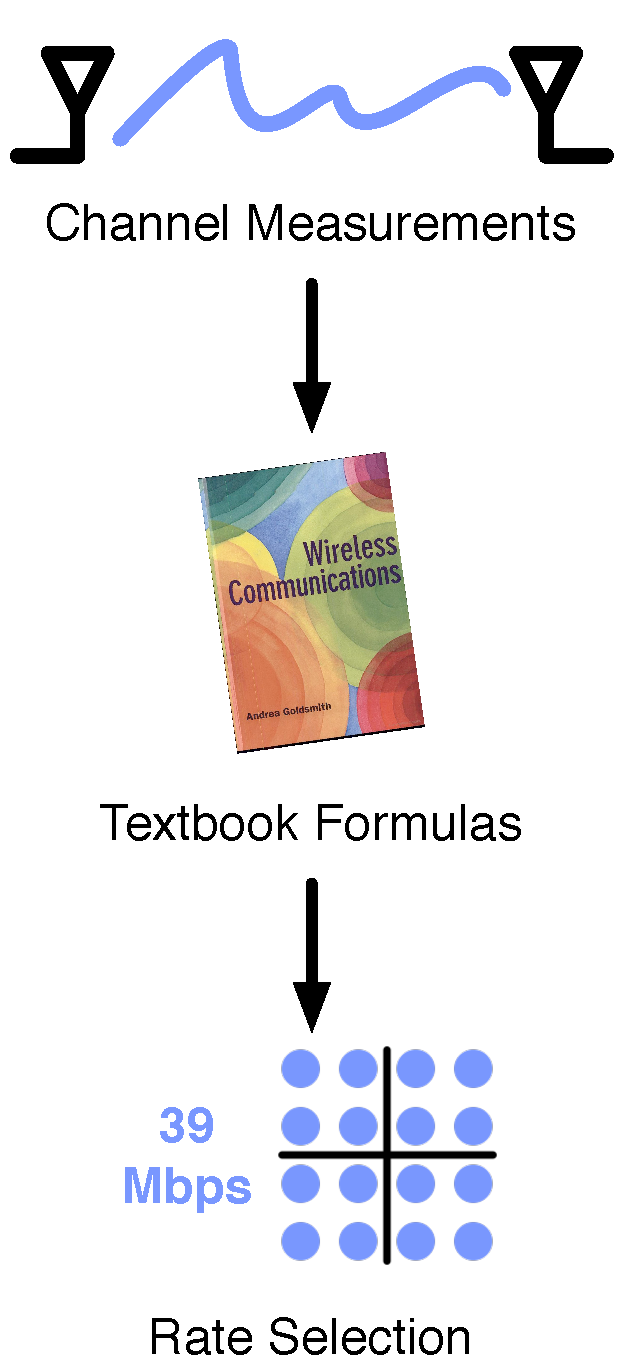
\includegraphics[width=2in]{figures/rate_selection_theory}
			\hspace{0.1in}
		}
			\hspace{0.1in}
		\subfigure[The probe-based approach to rate selection used in practice][The probe-based approach to rate selection used in practice.]{
			\hspace{0.1in}
			\label{fig:rate_selection_practice}
			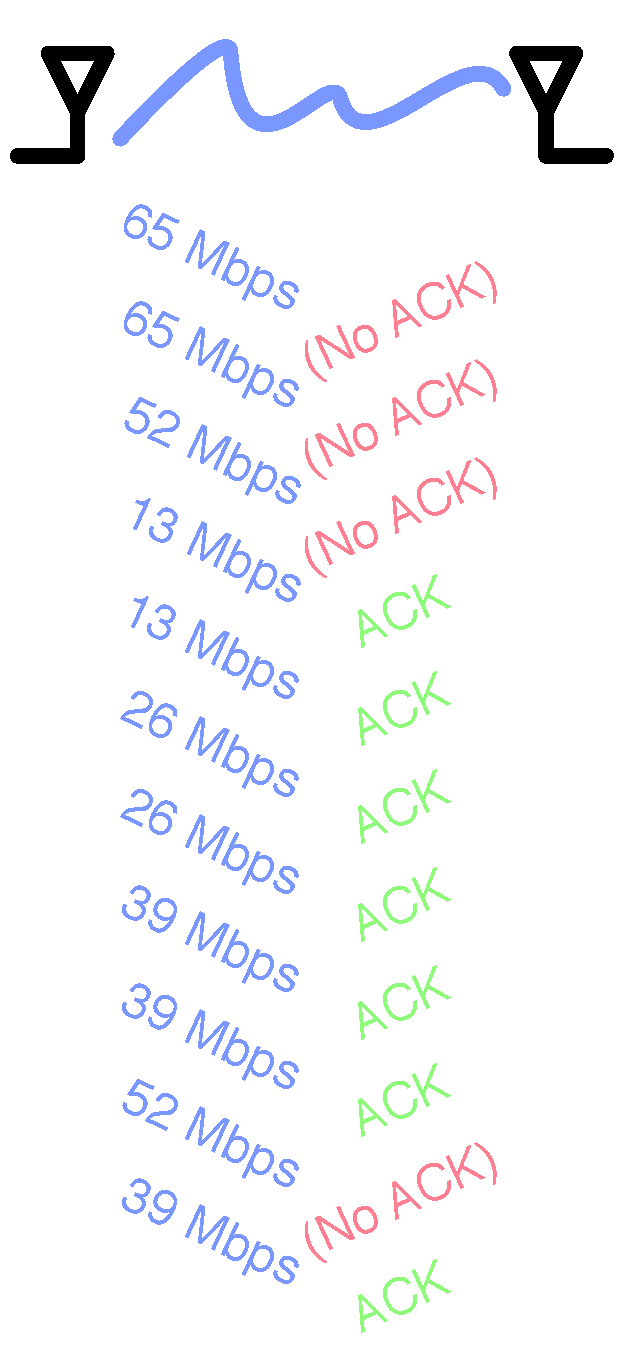
\includegraphics[width=2in]{figures/rate_selection_practice}
			\hspace{0.1in}
		}
	\caption[Approaches to rate selection]{\label{fig:rate_selection_algorithms}Approaches to rate selection.}%
\end{figure}

In practice, this approach has never worked for Wi-Fi links. The 802.11 standard defines a channel metric related to the SNR called the Receive Signal Strength Indicator, or RSSI, that captures the total amount of power in the channel and in most chipsets is indeed a direct measure of the SNR. However, Wi-Fi systems have never used RSSI as more than a coarse indicator of expected performance. There have simply been too many ways in which the observed measurements and actual performance fail to match the predictions of theory. For example, hardware estimates of RSSI can be mis-calibrated, the wireless channel can vary over packet reception, and can be corrupted by interference; all of these are known to be issues in practice~\cite{Camp_rateadapt,Judd_CHARM,Reis_interference}.

Since rate selection based on RSSI has never worked for Wi-Fi, practical systems use \define{rate adaptation} algorithms instead~\cite{Bicket_SampleRate,Minstrel,Wong_RRAA}. These algorithms, exemplified by \figref{fig:rate_selection_practice}, are guided search schemes that simply test individual rates to see how well they work. When the loss rate is too high, a lower rate is used; otherwise a higher rate is tested. This approach works well for slowly varying channels and simple links, since the best setting will soon be found.

However, remember the Wi-Fi trends we mentioned earlier: the transmit configuration of a single Wi-Fi link now includes not just rate, but additional dimensions that take into account the use of multiple antennas or channel widths, and these devices are increasingly being used while mobile. Thus algorithms to configure the rates of these links need to respond faster to match changing channels, while simultaneously choosing from among more possibilities. As a result, rate adaptation algorithms are getting less efficient as these systems change.

Thus far, I have described the challenges inherent to choosing an efficient rate to send data on a wireless link. On its own, this is a hard problem, but in addition, I note that rate is only one of many parameters to optimize for a Wi-Fi link. For instance, a transmitter may want to trim excess transmit power to both save energy and reduce interference at nearby receivers. Or a sender might improve a link by selecting a different subset of its transmit antennas, or by applying beamforming techniques to better match the signal to the radio channel. Finally, note that these parameters are not generally independent---changing any one of them can affect the best operating point for another. For instance, switching the operating frequency (of which there are often 10 to 20 options) can dramatically change the RF channel, and this in turn can affect which transmit antennas provide the best link, and how the transmitted signal should be shaped for maximum performance. All of these factors contribute to determining the best way to configure a link.

In practice, the solution taken by hardware/driver manufacturers today is to simply ignore most of these dimensions. For instance, only Intel's \program{iwlwifi} driver, out of all the 802.11n drivers in the Linux kernel driver, adapts the transmit antenna set in an online manner. Similarly, few access points and no clients adjust transmit power for ongoing links, instead opting to transmit at the maximum power and guarantee the best link. The solutions work well enough for wireless access point networks, mostly due to the simple way in which links are used today. Still, these solutions are inefficient for a single link---and in the next section, we will see that the problem gets even more complicated when performing network-level configuration of multiple devices that operate in multiple links.

\subsection{Configuring a Network of Devices}
\label{sec:intro_network_problems}
In this section, I will illustrate how a network of devices has a significantly larger configuration space than a single link. I frame this discussion using the examples in \figref{fig:network_examples}, which represent the three key network-level configuration problems that Wi-Fi Direct networks will have to solve to build rich device-to-device applications. Depending on the problem being solved, these configuration problems can have increased complexity that is linear in the number of devices (AP selection), quadratic (Multi-hop routing), or even exponential (Spatial reuse).

\begin{figure}[tp]
	\centering
	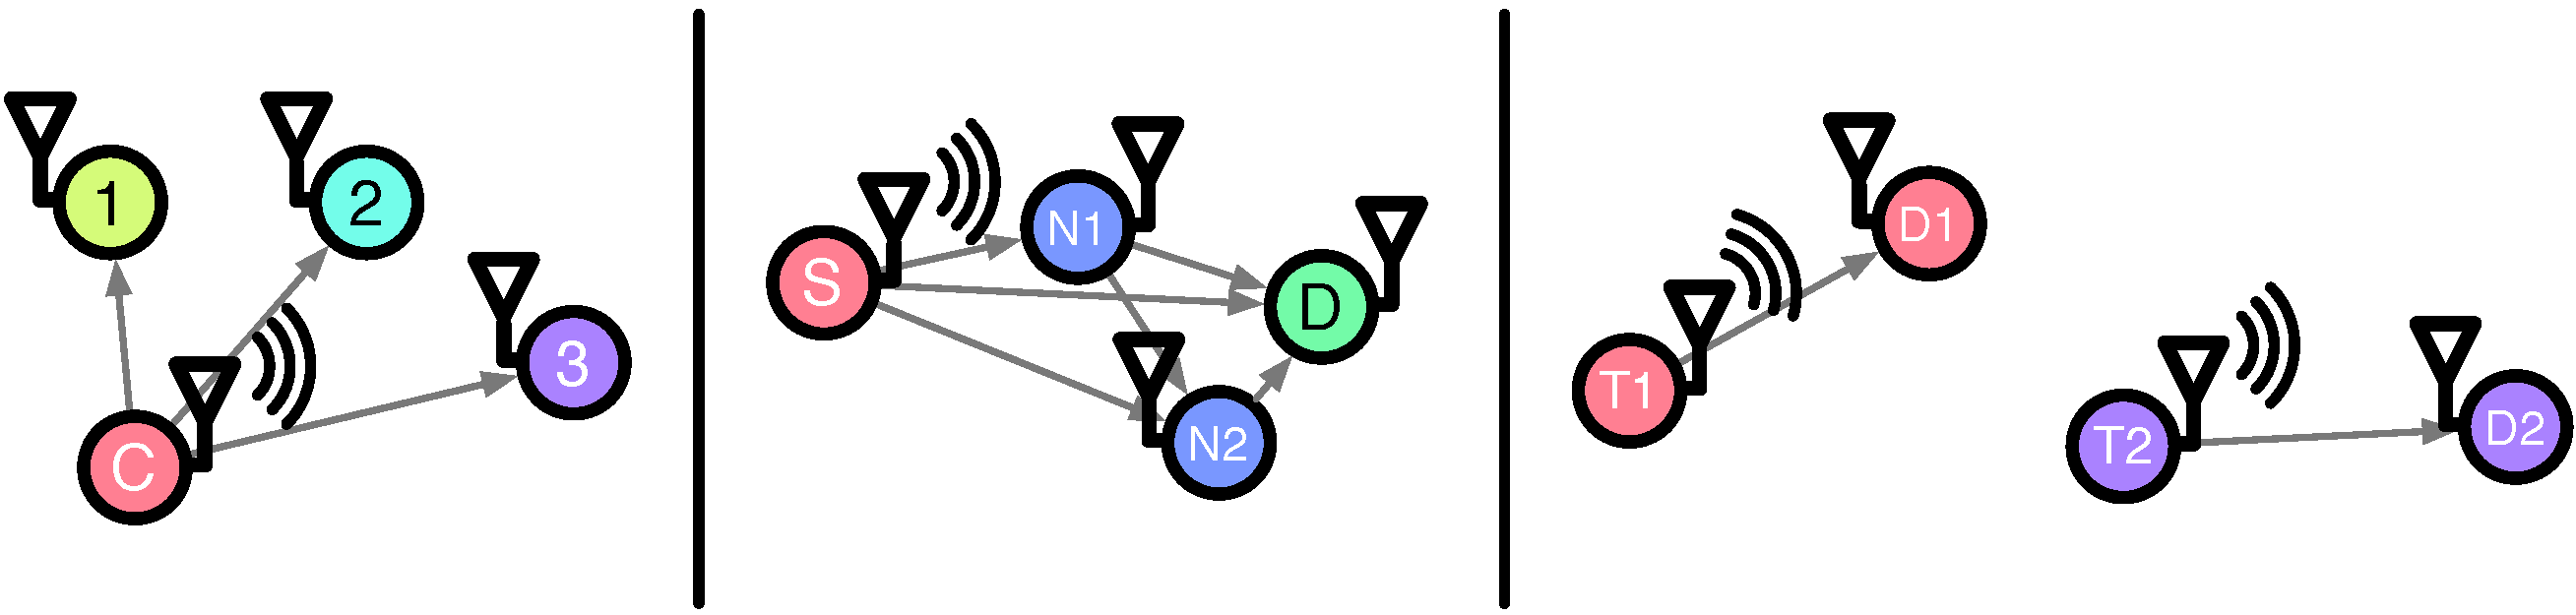
\includegraphics[width=\textwidth]{figures/network}
	\caption[The three key configuration problems in multi-device networks]{\label{fig:network_examples} The three key configuration problems in multi-device networks. \textit{Left:} access point selection. \textit{Center:} Multi-hop mesh routing. \textit{Right:} Spatial reuse. }
\end{figure}

\subsubsection{Access Point Selection}
In \figref{fig:network_examples}, on the left, the client $C$ wishes to join the network offered by the access points $AP_1$, $AP_2$, and $AP_3$. The \define{access point selection} problem is simple: the client should connect to the access point that provides the link with the best rate. But in order to choose correctly, the client must accurately evaluate the rate offered by each access point. This in turn means that the client must have a way to assess its rate to each access point rapidly, i.e., a solution to the rate selection problem described above. Testing all access points using a rate adaptation-like approach would take too long and would take airtime away from ongoing connections. In practice clients simply connect the access point with the highest SNR\@. This heuristic approach provides only an approximation to the optimal solution, and would benefit from a better way to predict performance over measured wireless channels.

\subsubsection{Multi-hop Mesh Routing}
In \figref{fig:network_examples}, in the middle, the source $S$ wishes to send data to the destination $D$, and nodes $N_1$ and $N_2$ are also present in the network. The \define{multi-hop routing} problem is to choose the best path through the network by which to deliver data from $S$ to $D$. In this case, many paths are available, such as the direct path $S\mendash D$, the one-hop paths $S\mendash N_1\mendash D$ and $S\mendash N_2\mendash D$, and finally $S\mendash N_1\mendash N_2\mendash D$. To evaluate the different paths, we need to know the rate available on each hop, which in this case would require knowing the rates of six different links. Once again, measuring the ground truth rate of each link by testing each configuration would likely take too long, and would add overhead to the network.

Practical work in this area primarily takes one of two approaches. Most of the wireless mesh research in the past decade avoided this problem by simply ignoring many of the dimensions of the configuration space. These papers not only used single antenna systems at fixed transmit powers, but also typically fixed the entire network to a single rate. The alternative approach, taken by a few recent papers, has been to collected statistics about packet delivery between all pairs of nodes for different rates, and estimate the rate from the measured SNR for links without sufficient statistics. These recent works have exclusively handled single-antenna 802.11a/b/g networks, and would likely be forced to rely on SNR-based rate predictions if the underlying links used 802.11n instead.

\subsubsection{Spatial Reuse}
The third example, shown in \figref{fig:network_examples}, is the \define{spatial reuse} problem. Here, two independent links both wish to communicate at the same time and in the same frequency, and need to share the wireless medium. If the links share the medium, for example each using half the airtime, then each gets half of the rate as if they were operating alone. In certain situations, depending on the placement of the four devices and the amount of interference between links, it may provide more total throughput for the links to send concurrently, each using all of the airtime but maybe using a slightly lower rate.

Once again, deciding which of these two possibilities is better requires the system to predict the rate on multiple different links. In this case, the rate needs to be predicted not only for each link in isolation, but also for every possible pair of configurations of the links. In this case, and unlike the prior two problems, the size of the resulting configuration space is the product of the sizes of the space of each individual link. As a result%, CMAP~\cite{Vutukuru_CMAP} and CENTAUR~\cite{Shrivastava_CENTAUR},
practical works on spatial reuse for Wi-Fi has simply fixed the entire network to a single rate during experiments.

\subsection{Summary}
In this section, I first showed that the configuration problems for a single link have grown dramatically with the switch to 802.11n technology, and then presented the three key network-level configuration problems for Wi-Fi Direct-like networks and explained why their solution space is even larger than for a single link. The main conclusion from this section is that the heuristic and adaptation-based approaches used in the simple network problems solved today will likely not scale to these bigger problems. (I will demonstrate this later in the thesis in \chapref{chap:applications}). Instead, what we need is a way to accurately and rapidly assess the quality of links for all the factors mentioned in \secref{sec:intro_single_link_problems}, and use this process to inform joint optimization problems such as those described in \secref{sec:intro_network_problems}. I present my approach to solving this problem in the next section.

%Depending on the problem being solved, these configuration problems can have increased complexity that is linear in the number of devices (AP selection), quadratic (Multi-hop routing), or even exponential (Spatial reuse). 
%Additionally, these scenarios tend to differ from the single link case in that their solutions can not be fluidly adapted while online. For instance, a transmitter on a single link could rapidly adapt its rate or antenna selection, and a poor choice will be rapidly corrected. Conversely, a client in today's wireless networks cannot switch between access point at short time scales. Thus it is especially important that these network-level decision problems are made accurately the first time.

%%%%%%%%%%%%%%%%%%%%%%%%%%%%%%%%%%
\section{Approach}
\label{sec:intro_approach}
My approach to the Wi-Fi network configuration problem is to return to the basic channel measurement-based strategy of selecting configurations for wireless networks. In particular, my hypothesis is that it is possible to use theory to connect the performance of 802.11 devices on real links to measurements of their underlying radio channels in practice. In this thesis, I will demonstrate that channel measurements readily available in 802.11n Wi-Fi devices can be used to predict packet delivery over real 802.11n links, and that these predictions are sufficiently accurate to inform decisions about wireless network device configurations.

\subsection{Better physical layer measurements}
I noted earlier that the packet-level SNR metric computed from RSSI has never been used as an accurate predictor of packet delivery for 802.11 networks, and I will present experimental data that confirms this effect in a succeeding chapter (\chapref{chap:problem}). If hardware estimates of RSSI are not sufficiently accurate, then what data source can we use instead?

The 802.11n standard released in 2009 adds a new Channel State Information (CSI)~\cite[\S7.3.1.27]{80211n} measurement facility in order to support multi-antenna (Multiple-Input-Multiple-Output, or MIMO) operation. Devices that report the CSI can provide channel measurements at the level of individual OFDM subcarriers and individual spatial paths. These measurements form a much richer set of information about the RF channel than does the RSSI.

To compare the CSI with SNR, consider an 802.11n link with $M$ antennas at the transmitter and $N$ at the receiver. Today's receivers measure $N$ RSSI values, each corresponding to the total power measured at one receive antenna. In contrast, the CSI contains $M$$\times$N$\times$$S$ values, where $S$ is the number of subcarriers measured. This results in a factor of $MS$ more channel measurements when measuring CSI as opposed to SNR\@. In 802.11, the CSI can measure from 1 to 4 antennas, and from 16 to 114 subcarriers. The CSI thus includes between 16$\times$ and $456\times$ as many measurements as the RSSI\@.

%\item Second, the quality of Wi-Fi hardware has improved dramatically. Manufacturers typically calibrate chipsets across a wide range of conditions, including temperature and transmit power level, in order to meet regulatory requirements, to meet standardized tolerances, and to maximize performance. The modern use of OFDM and MIMO techniques additionally enables channel estimates that are less susceptible to interference than spread-spectrum modulation (because of lower correlation), and can be taken more rapidly.

\subsection{A practical Effective SNR model for 802.11n}
The CSI gives fine-grained channel measurements that capture the low-level details of the physical RF channel, but this does not on its own give an accurate predictor of packet delivery. However, there is a recent body of theoretical work on measuring and predicting the error performance of wireless channels that are faded, use OFDM, or use MIMO\@. Chief among these is the seminal 1998 paper by Nanda and Rege on the concept of \define{Effective $E_b/N_0$}~\cite{Nanda_EffectiveSNR},\footnote{In electrical engineering literature, $E_b$ denotes the energy of a bit and $N_0$ denotes the noise floor, so $E_b/N_0$ is the signal-to-noise ratio of a single bit. In the context of 802.11, in which SNR is derived from RSSI, we use a slightly different definition of SNR that is not normalized by the number of bits.} which forms the theoretical basis of my model for 802.11n MIMO-OFDM channels. In this thesis, I build a practical Effective SNR-based model that uses CSI measurements from commodity 802.11n devices and makes accurate predictions about 802.11n packet delivery.

I give a detailed description of the Effective SNR concept and how I model it in a practical system in a subsequent chapter (\chapref{chap:model}). Briefly, the goal of the Effective SNR is to to give a channel quality metric that reflects the \emph{actual error rate of the link} taking into sub-channel effects like fading. The Effective SNR of a faded channel is defined as the SNR in an equivalent constant-SNR channel that would yield the same error performance. Another way to think about this is that the SNR reports the \emph{total power} received, whereas the Effective SNR reports the amount of \emph{useful power} received. As I will show in this thesis, because Effective SNR accurately reflects packet delivery it can be used to inform a wide variety of configuration decisions about 802.11n systems.

\begin{figure}[t]
	\centering
	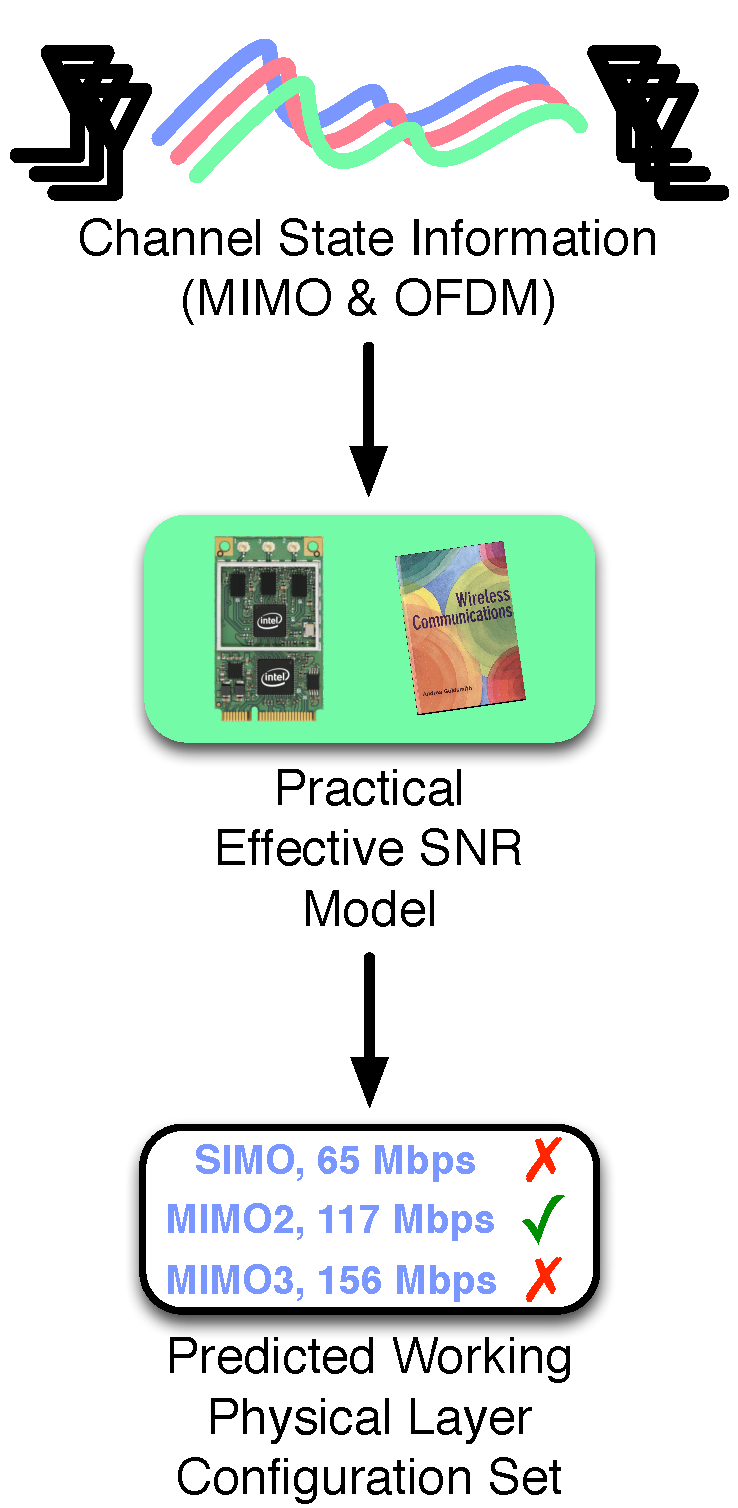
\includegraphics[width=2.2in]{figures/selection_esnr}
	\caption[Effective SNR-based approach to making application decisions]{\label{fig:selection_esnr}An Effective SNR-based approach to making application decisions in 802.11n networks.}
\end{figure}

\subsection{Approach overview}
I present the basic outline of my Effective SNR-based approach to informing configuration of 802.11n systems in \figref{fig:selection_esnr}. This approach is closely related to the ``theoretical approach'' presented in \figref{fig:rate_selection_theory}, with a few differences.

As a first step, a client will measure the CSI for an 802.11n wireless link to capture the fine-grained channels details at the level of frequency-selective fading (to understand performance under OFDM) and independent spatial paths (to understand performance when using MIMO). Second, the measured CSI will be used as input to my practical Effective SNR-based model for 802.11n packet delivery. This model incorporates textbook algorithms, ideas from communications theory, as well as some implementation-specific details to handle a wide variety of channels, hardware devices, and applications. Finally, the output of the model is a predicted \emph{set of working physical layer configurations}. For each physical layer configuration in the application space---which can span the choice of modulation, coding scheme, transmit or receive antenna set, and more---the model predicts whether that configuration is likely to deliver packets reliably. The application can then choose among the working configurations in a way that optimizes its objective function.

Throughout this thesis, I describe the components of this approach in detail. The organization of this thesis is presented below in \secref{sec:intro_organization}.

%In my thesis, I take advantage of these three points to build a practical system to return to the ``traditional'' algorithm and predict wireless error performance from channel measurements. Rather than the ``try-it-and-see'' adaptation algorithms in use today, my model enables measurement-based selection of operating points for a wide range of transmitter and receiver parameters over a large application space.

%The opportunity to make progress has arisen for two reasons. First, 802.11n devices measure the channel at the level of individual OFDM subcarriers and individual spatial paths to support 802.11n MIMO (multi-antenna) operation. They report this information in a standard Channel State Information (CSI) format~\cite[\S7.3.1.27]{80211n}. This provides a much richer source of information than SNR\@. Note that this CSI naturally applies to 802.11a/g rates because they are a subset of 802.11n rates. Second, modern NICs use OFDM, which gives channel estimates that are less susceptible to interference than spread spectrum (because of lower correlation), and are calibrated. Both factors lead to more meaningful measurements than in the past.


%\subsubsection{Better Channel Measurements}
%The chief problems with using channel measurements available in commodity Wi-Fi devices is that they only describe the SNR, a measure of total power in the channel. Even if they didn't suffer from the hardware artifacts described above, this information would insufficiently describe the wireless channel, because bits are no longer spread across the entire band as in 802.11b modes, but instead are sent independently on different frequencies (called subcarriers) with orthogonal frequency division multiplexing (OFDM), and on different spatial paths with 802.11n multi-antenna techniques.
%
%As part of my thesis, I built a tool (described in \secref{sec:tool}) to measure the channel in a fine-grained manner that accurately reflects the underlying radio channel. In particular, this tool can measure the 802.11n Channel State Information (CSI)~\cite[\S7.3.1.27]{80211n} for each received 802.11n packet. The CSI measures not just the SNR of the entire channel, but instead the channel response at the level of individual subcarriers and spatial paths. For comparison, for an 802.11n link with the antennas each at the transmitter and receiver, today's receivers measure three SNR values each corresponding to the total power measured at a receive antenna. In contrast, the CSI contains 3$\times$3$\times$$S$ values, where $S$ is the number of subcarriers measured. Since 802.11n links use either 56 or 114 subcarriers, $S$ could be as high as 56; in practice, our tool can only measure a subset of 30 of them. Still, this results in 270 channel measurements using the CSI, compared to only 3 with the traditional SNR\@.
%My tool uses a commercially-available Intel Wi-Fi device that supports 802.11n. I modified the open-source Linux drivers, and---in conjunction with Intel Research---the firmware for these devices to enable debug modes with 
%\subsubsection{Effective SNR}


%%%%%%%%%%%%%%%%%%%%%%%%%%%%%%%%%%
\section{Contributions}
\label{sec:intro_contributions}

The contributions of this thesis are threefold:
\begin{itemize}
\item First, I develop a model that uses the 802.11n CSI to predict the error performance of different transmitter configurations on the wireless channel. This model is flexible to support a wide variety of transmitter and receiver device capabilities, device implementations, and applications. I also detail how to use this model in a system that can solve a large number and variety of configuration problems similar to those described in \secref{sec:intro_problem}.
\item Second, I present an implementation of this system using a commodity 802.11n wireless device that demonstrates its feasibility in practice and handles the practical considerations of operation over real links using real, non-ideal hardware. This includes a detailed experimental evaluation of my system that shows that this model accurately predicts packet delivery over real 802.11n wireless links in practice.
\item Third, I evaluate this system in the context of a wide variety of 802.11n applications, and quantify the application performance gains when using my Effective SNR metric over versions that use the RSSI-based SNR channel measurements available today.
\item Finally, as part of my thesis I have produced an 802.11n research platform based on open-source Linux kernel drivers, open-source application code, and commodity Intel 802.11n devices using closed-source firmware that I customized.
%that uses commodity 802.11n wireless devices to measure the 802.11n CSI for the wireless channel, and use this tool to apply my model to real measured 802.11n channels.
I have released this tool publicly, and at the time of writing it is in use at 19 universities, research labs, and corporations.
\end{itemize}

%%%%%%%%%%%%%%%%%%%%%%%%%%%%%%%%%%
\section{Organization of this Thesis}
\label{sec:intro_organization}
This thesis is organized as follows. In \chapref{chap:background}, I provide background information on wireless signals and systems in general, and the IEEE 802.11 standards in particular. \chapref{chap:problem} introduces the problem with using channel measurements to predict wireless link performance in today's hardware and using today's techniques, and introduces my Effective SNR-based approach to solving it. In \chapref{chap:model}, I develop my Effective SNR model for 802.11n link performance, and demonstrate its ability to handle a wide range of transmitter and receiver configurations as well as wireless applications. I then describe my measurement tool, experimental apparatus, and basic measurements in \chapref{chap:tool}, and then use these measurements to evaluate the ability of my model to predict error performance over a single link in \chapref{chap:delivery}. Next, I conduct a detailed study of the model in the context of rate selection for 802.11n in \chapref{chap:rate}, and then present brief results for a variety of other applications in \chapref{chap:applications}. I place this thesis in the context of related work in \chapref{chap:related}. Finally, I present a brief discussion of the next steps for this work along with concluding thoughts in \chapref{chap:conclusion}.

%%%%%%%%%%%%%%%%%%%%%%%%%%%%%%%%%%
\ifx\mainfile\undefined
%
% ==========   Bibliography   ==========
%
%\nocite{*}   % include everything in the uwthesis.bib file
\bibliographystyle{plain}
\bibliography{dhalperi_thesis}

\end{document}
\fi

\ifx\mainfile\undefined
%  ========================================================================
%  Copyright (c) 2006-2011 The University of Washington
%
%  Licensed under the Apache License, Version 2.0 (the "License");
%  you may not use this file except in compliance with the License.
%  You may obtain a copy of the License at
%
%      http://www.apache.org/licenses/LICENSE-2.0
%
%  Unless required by applicable law or agreed to in writing, software
%  distributed under the License is distributed on an "AS IS" BASIS,
%  WITHOUT WARRANTIES OR CONDITIONS OF ANY KIND, either express or implied.
%  See the License for the specific language governing permissions and
%  limitations under the License.
%  ========================================================================
%
 
\documentclass [11pt, twoside] {uwthesis}

\usepackage{color}
\usepackage{url}
\usepackage{amsmath}
\usepackage{amsfonts}
\usepackage[bookmarks,
	hidelinks,
	plainpages=false,
	pdfpagelabels,
	pagebackref=true,
            ]{hyperref}
\renewcommand*{\backref}[1]{}% for backref < 1.33 necessary
\renewcommand*{\backrefalt}[4]{%
  \ifcase #1 %
    (No citations.)%
  \or
    (Cited on page #2.)%
  \else
    (Cited on pages #2.)%
  \fi
}

\newcommand{\biburl}[1]{{\tt<}\url{#1}{\tt>}}

\hypersetup{%
pdfauthor = {Daniel Chaim Halperin},
pdftitle = {Simplifying the Configuration of 802.11 Wireless Networks with Effective SNR},
pdfsubject = {Ph.D. Dissertation},
pdfkeywords = {},
pdfcreator = {University of Washington, Computer Science and Engineering},
pdfproducer = {},
bookmarksopen = {true},
pdfpagelayout = {TwoColumnRight},
}

\usepackage{footnotebackref}
%%%%%%%%%%%%%%%%%%%%%%%%%%%%%%%%%%%%%%%%%%%%%%%%%%%%%%
%%%        Formatting sections                     %%%
%%%%%%%%%%%%%%%%%%%%%%%%%%%%%%%%%%%%%%%%%%%%%%%%%%%%%%
\newcommand{\algref}[1]{Algorithm~\ref{#1}}
\newcommand{\chapref}[1]{Chapter~\ref{#1}}
\renewcommand{\eqref}[1]{Equation~\ref{#1}}
\newcommand{\figref}[1]{Figure~\ref{#1}}
\newcommand{\secref}[1]{\S\ref{#1}}
\newcommand{\tabref}[1]{Table~\ref{#1}}
\newcommand{\heading}[1]{\vspace{4pt}\noindent\textbf{#1}}
\newcommand{\topheading}[1]{\noindent\textbf{#1}}
\newcommand{\noheading}[0]{\vspace{4pt}\noindent}

%%%%%%%%%%%%%%%%%%%%%%%%%%%%%%%%%%%%%%%%%%%%%%%%%%%%%%
%%%        XXX and other warnings                  %%%
%%%%%%%%%%%%%%%%%%%%%%%%%%%%%%%%%%%%%%%%%%%%%%%%%%%%%%
\newcommand{\xxx}[1]{\textit{\color{red}XXX #1}}

%%%%%%%%%%%%%%%%%%%%%%%%%%%%%%%%%%%%%%%%%%%%%%%%%%%%%%
%%%        Units                                   %%%
%%%%%%%%%%%%%%%%%%%%%%%%%%%%%%%%%%%%%%%%%%%%%%%%%%%%%%
\usepackage{xspace}
\newcommand{\unitsep}{\texorpdfstring{\,}{ }}
\def\unit#1{% from: http://www.tex.ac.uk/cgi-bin/texfaq2html?label=csname "Defining a macro from an argument"
  \expandafter\def\csname #1\endcsname{\unitsep\text{#1}\xspace}%
}
\def\varunit#1#2{% from: http://www.tex.ac.uk/cgi-bin/texfaq2html?label=csname "Defining a macro from an argument"
  \expandafter\def\csname #1\endcsname{\unitsep\text{#2}\xspace}%
}
\unit{GHz}
\unit{MHz}
\unit{kHz}
\unit{Gbps}
\unit{Mbps}
\unit{KB}
\unit{dB}
\unit{dBi}
\unit{dBm}
\unit{W}
\unit{mW}
\varunit{uW}{$\mu$W}
\unit{ms}
\varunit{us}{$\mu$s}
\unit{h}
\unit{m}
\unit{s}
\unit{km}
\unit{cm}
\unit{mm}
\varunit{mmsq}{mm$^\text{2}$}
\varunit{insq}{in$^\text{2}$}
\newcommand{\degree}{\ensuremath{^\circ}\xspace}
\newcommand{\degrees}{\degree}
%%%%%%%%%%%%%%%%%%%%%%%%%%%%%%%%%%%%%%%%%%%%%%%%%%%%%%%%%%%%%%%%%%%%%%%%%%%%%%%%%%%%%%
% Euler for math | Palatino for rm | Helvetica for ss | Courier for tt
%
% From: http://www.tug.org/mactex/fonts/LaTeX_Preamble-Font_Choices.html
%%%%%%%%%%%%%%%%%%%%%%%%%%%%%%%%%%%%%%%%%%%%%%%%%%%%%%%%%%%%%%%%%%%%%%%%%%%%%%%%%%%%%%
\renewcommand{\rmdefault}{ppl} % rm
\usepackage[scaled]{helvet} % ss
\usepackage{courier} % tt
\usepackage{eulervm} % a better implementation of the euler package (not in gwTeX)
\normalfont
\usepackage[T1]{fontenc}
%%%%%%%%%%%%%%%%%%%%%%%%%%%%%%%%%%%%%%%%%%%%%%%%%%%%%%%%%%%%%%%%%%%%%%%%%%%%%%%%%%%%%%

%%%%%%%%%%%%%%%%%%%%%%%%%%%%%%%%%%%%%%%%%%%%%%%%%%%%%%
%%%        Figures                                 %%%
%%%%%%%%%%%%%%%%%%%%%%%%%%%%%%%%%%%%%%%%%%%%%%%%%%%%%%
\usepackage{graphicx}
% Caption package both lets you set the spacing between figure and caption
% and also makes the \figref{} point to the right place.
\usepackage[font=bf,aboveskip=6pt,belowskip=-4mm]{caption}
% Allow subfigures, make them bold
\usepackage[bf,BF,small]{subfigure}
% List of figures
\setcounter{lofdepth}{2}  % Print the chapter and sections to the lot

%%%%%%%%%%%%%%%%%%%%%%%%%%%%%%%%%%%%%%%%%%%%%%%%%%%%%%
%%%        Lists with reduced spacing              %%%
%%%%%%%%%%%%%%%%%%%%%%%%%%%%%%%%%%%%%%%%%%%%%%%%%%%%%%
\usepackage{enumitem}

%%%%%%%%%%%%%%%%%%%%%%%%%%%%%%%%%%%%%%%%%%%%%%%%%%%%%%
%%%        Fancy tables                            %%%
%%%%%%%%%%%%%%%%%%%%%%%%%%%%%%%%%%%%%%%%%%%%%%%%%%%%%%
\usepackage{tabulary}
\usepackage{booktabs}

%%%%%%%%%%%%%%%%%%%%%%%%%%%%%%%%%%%%%%%%%%%%%%%%%%%%%%
%%%        Formatting techniques/tools/etc.        %%%
%%%%%%%%%%%%%%%%%%%%%%%%%%%%%%%%%%%%%%%%%%%%%%%%%%%%%%
\newcommand{\term}[1]{\texttt{#1}}

\begin{document}
 
\textpages
\setcounter{chapter}{1} % Set to n-1!
\fi
%%%%%%%%%%%%%%%%%%%%%%%%%%%%%%%%%%

\cleardoublepage
\chapter{Background}
\label{chap:background}

In this chapter, I establish the fundamentals of wireless communication and the IEEE 802.11 standards to the extent needed to understand my thesis.

\section{Digital Communication Principles}
Electromagnetic (EM) communications, which send data using \define{electromagnetic signals}, form the basis of the technologies I will discuss in this thesis. One key aspect of each wireless technology is which part of the electromagnetic spectrum it uses, characterized by its \define{carrier frequency or center frequency}, denoted $f$. A fundamental property of radio waves is that the frequency of a wave determines its \define{wavelength} $\lambda$ according to the relationship $c=f\lambda$, where $c$ is the speed of light. IEEE~802.11 networks typically use EM signals with a carrier frequency in the range of 2.4\GHz and 5\GHz and corresponding wavelengths of about 12\cm and 6\cm.

Data transmission using EM signals works by \define{modulating} a pure sine wave with frequency $f$, i.e.\ by transforming the sine wave to reflect the underlying data. The simplest modulation scheme might be to turn the sine wave on or off depending on whether the bit to be transmitted is a 1 or a 0. The rate at which the transmitter varies the signal---in this example, the rate the sine wave is turned on or off---is called the \define{symbol rate}, and determines the \emph{bandwidth} of the channel $B$ measured in Hertz (Hz).

The \emph{amplitude} of the sine wave, e.g. how much the peak varies from the zero (usually measured in volts (V)), determines the \define{power} of the signal. These two quantities are related by a quadratic relationship: doubling the amplitude of a signal results in a quadrupling of the signal power.

In a \define{link}, that is a sender communicating data to a receiver, the sender generates a signal with \define{transmit (signal) power} level $T$ that propagates through the \define{channel} connecting the two. The channel could be a \define{wire} or it could be the free-space \define{radio frequency (RF)} environment in which signals propagate from the transmitter's antenna to the receiver's antenna over the air.

\subsection{The Wired Channel}
To simplify the discussion, I will start with the case of a wired channel. The transmitted signal propagates down the wire to the receiver and then is received with \define{receive (signal) power} $S$. While propagating through the wire, the signal gets slightly weaker as a small amount of energy is absorbed. The net effect of this absorption is called \define{attenuation}, denoted $\alpha$, and is defined mathematically as the multiplicative decrease in power induced by the channel:
\begin{equation}
	\label{eq:attenuation}
	\alpha = \frac{T}{S}.
\end{equation}
In addition to attenuation, the wired channel also induces a \define{phase shift} as the electromagnetic signal propagates. The value of this phase shift, denoted $\theta$, depends on factors including the length of the wire and the frequency of the signal, and is generally considered to be an unknown, uniformly random quantity between $0$ and $2\pi$.

\begin{table}
\centering
\begin{tabular}{cll}
\toprule%
Variable & Meaning & Units\\
\midrule%
$f$ & Frequency & Hz \\
$\lambda$ & Wavelength & m \\
$B$ & Bandwidth & Hz \\
$T$ & Transmit signal power & dBm (decibels relative to 1 milliwatt) \\
$S$ & Receive signal power & dBm \\
$\alpha$ & Attenuation & dB (decibels, unitless) \\
$\theta$ & Phase & radians \\
$N$ & Noise power & dBm \\
$K$ & Temperature & kelvins \\
$\rho$ & Signal-to-noise ratio (SNR) & dB \\
$R$ & Shannon Capacity & bits \\
$d$ & Distance & m \\
$n$ & Path loss exponent & unitless \\
$I$ & Interference power & dBm \\
$\rho_I$ & SINR & dB \\
$M$ & Number of transmit antennas & (antennas) \\
$N$ & Number of receive antennas & (antennas)\\
\bottomrule
\end{tabular}
\caption[Table of notation used in this chapter]{\label{tab:bg_notation}Table of notation used in this chapter.}
\end{table}

The signal measured by the receiver is also corrupted by broad-spectrum electromagnetic noise. This corruption is sometimes called \define{Johnson-Nyquist noise} after its identification in 1927 by Johnson~\cite{Johnson_noise} and explanation in 1928 by Nyquist~\cite{Nyquist_noise}, but it is more commonly known as \define{thermal noise}. Thermal noise can be modeled as a complex Gaussian with average \define{noise power} $N$ (in Watts) equal to
\begin{equation}
\label{eq:noise}
N = kKB,
\end{equation}
where $k\approx1.38\times10^{-23}$ (in Joules/kelvin) is Boltzmann's constant, $K$ is the temperature (in kelvins), and $B$ is the bandwidth. This is called additive, white Gaussian noise (AWGN).
%For a device at room temperature ($\approx$ 293\K), we can compute $N$ in dBm using the approximation
%\begin{equation}
%N \text{ (dBm)} = -174 + 10\log_{10}(B).
%\end{equation}

In the context of 802.11, we typically measure power-related quantities on a logarithmic scale to capture the wide range of possible values. Power levels such as the quantities $T$, $S$, and $N$ are usually measured in decibels relative to 1~milliwatt, or dBm, and typically take on values like $T=20\dBm$ (100\mW) and $S=-80\dBm$ ($10^{-8}$\mW or 10\pW). To calculate $N$, we can use \eqref{eq:noise}: Wi-Fi links typically use bandwidths $B$ of 20\MHz or 40\MHz, which correspond to thermal noise levels of $-$101\dBm and $-$98\dBm at room temperature. In practice, the total noise is assumed to be thermal noise plus a 5\dB--15\dB \define{noise figure}, which is a quantity that estimates additional error added by imperfect analog hardware used in receiver processing. The total noise for a 20\MHz Wi-Fi channel might then be in the range of $-91$\dBm.

Now that we have defined the signal and noise powers, we can discuss the limits of the communication channel. In their seminal works, Ralph Hartley~\cite{Hartley_law} and Claude Shannon~\cite{Shannon_coding,Shannon_capacity} proved that the \define{capacity} of a channel---i.e., the maximum data rate $R$ at which the transmitter and receiver can communicate---is determined by the channel's bandwidth and its \define{signal-to-noise ratio (SNR)}. The SNR, denoted by $\rho$, is a unitless quantity typically measured in decibels and calculated as
\begin{equation}
\rho = \frac{S}{N}.
\end{equation}
For the example signal power of $-80\dBm$ and noise power of $-91\dBm$, this corresponds to an SNR of $11\dB$.


The Shannon-Hartley Theorem~\cite{Shannon_capacity} establishes what is called the \define{Shannon capacity} to be
\begin{equation}
\label{eq:shannon_capacity}
R = B\log_2(1+\rho).
\end{equation}
\figref{fig:shannon} shows this relationship for the normalized quantity $R/B$.

\begin{figure}[tb]
\centering
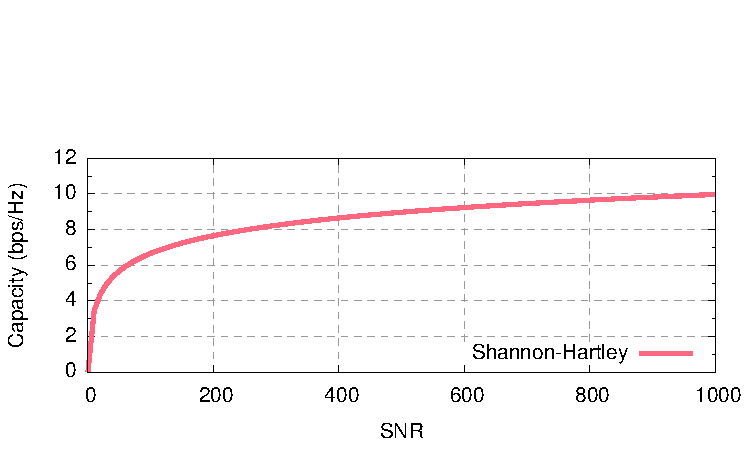
\includegraphics{calculations/shannon}\hspace{0.65in}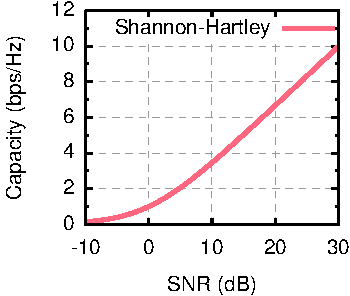
\includegraphics{calculations/shannon_log}\hspace{0.1in}
\caption[The Shannon Capacity of a communications channel with Gaussian noise]{\label{fig:shannon}The Shannon Capacity of a communications channel with Gaussian noise, presented in both linear and logarithmic (dB) scales.}
\end{figure}

The Shannon-Hartley Theorem determines a bound on the maximum rate achievable as a function of the bandwidth and signal strength. However, it does not give a practical scheme that realizes this bound, and instead systems like 802.11 use many different modulations that achieve different points along the $y$-axis, and choose among these in practice depending on the underlying channel conditions.

Note that for real links, the values of $S$ and $N$ are not known a priori. Instead, transmitters choose an encoding, and the receiver will be able to decode it successfully if the choice falls below the curve for the SNR experienced. The general problem of choosing the modulation to use, as well as the selection of other physical layer parameters, is the focus of my thesis. I describe this problem in more detail in the next chapter.

The binary modulation system I discussed above is a scheme called On-Off Keying~(OOK\@). Each symbol conveys 1 bit, and since the symbol rate is directly tied to the bandwidth used by a scheme, OOK can deliver at most 1 bps/Hz. A generalized form of OOK is Amplitude Shift Keying~(ASK\@), which can send more bits per symbol using multiple power levels. $m$-ASK, i.e., ASK with $m$ power levels per symbol, can deliver up to $\log_2(m)$ bits per symbol and thus can achieve a higher capacity.

\begin{figure}[t]
\centering
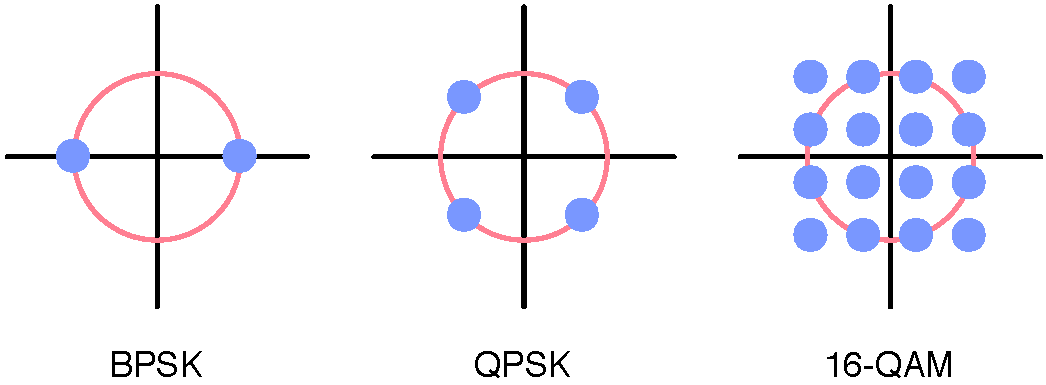
\includegraphics[width=0.9\textwidth]{figures/constellations_radius}
\caption[Constellation diagrams for the BPSK, QPSK, and 16-QAM modulations]{\label{fig:constellations}Constellation diagrams for the BPSK, QPSK, and 16-QAM modulations. These constellations are normalized such that each modulation has equal average transmit power, indicated by the red circle.}
\end{figure}

As mentioned above, electromagnetic signals actually have both an amplitude and a phase. Amplitude modulation varies one of these parameters, and a complementary scheme called Phase-Shift Keying~(PSK) keeps the amplitude constant but varies the phase. A third scheme known as Quadrature Amplitude Modulation~(QAM) varies both parameters simultaneously and results in a more efficient system when sending more than 2 bits per symbol. Noting that the polar coordinates given by amplitude and phase can equivalently be thought of as a complex number, $m$-QAM can be equivalently thought of as $\sqrt{m}$-ASK in both the real and complex dimensions simultaneously. \figref{fig:constellations} shows the two-dimensional \define{constellations} that result from picturing the symbols sent in BPSK (i.e.\ 2-PSK), QPSK (i.e.\ 4-PSK), and 16-QAM modulation schemes.

There are many more modulation schemes than I have presented here, but PSK and QAM are the modulations applicable to 802.11.
%Currently, Wi-Fi devices transmit data using 2-PSK (called Binary PSK, or BPSK), 4-PSK (called Quadrature PSK\@, or QPSK\@), 16-QAM\@, or 64-QAM\@.
64-QAM is the highest modulation currently used by Wi-Fi devices, though the future IEEE 802.11ac amendment~\cite{80211ac} will add 256-QAM to this set.

Recall that the signal will be corrupted by noise when measured at the receiver. Under the standard AWGN model, we model this corruption as shifting the received symbol by a random complex vector whose length depends on the noise power. We see in \figref{fig:constellations} that the different modulations have different constellation densities: the symbols of 16-QAM are clustered more closely than the symbols of QPSK or BPSK. This means that higher constellations which encode more bits per symbol are more vulnerable to noise. At low SNR, the receiver cannot easily distinguish between many symbols, so slower modulations with fewer constellation points should be used. At high SNR, the receiver can distinguish between more symbols and thus can use a denser constellation.

\begin{figure}[t]
\centering
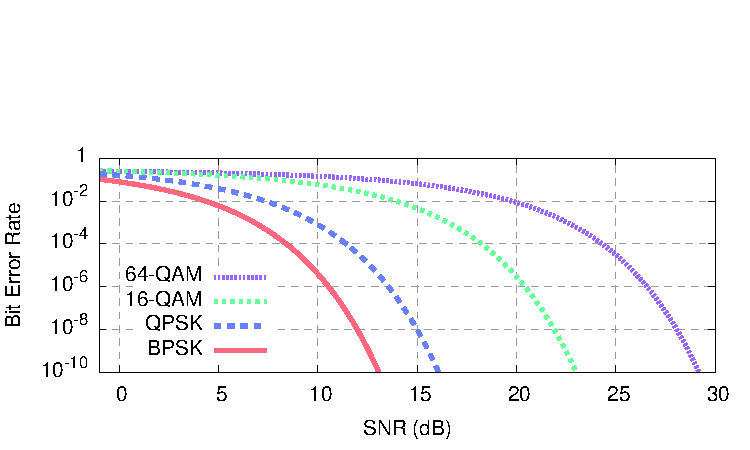
\includegraphics{calculations/snr_ber}
\caption[BER vs SNR for the four 802.11n modulation schemes]{\label{fig:mod_ber_snr}The relationship between bit error rate and SNR for the four 802.11 modulation schemes.}
\end{figure}

\begin{figure}[t]
\centering
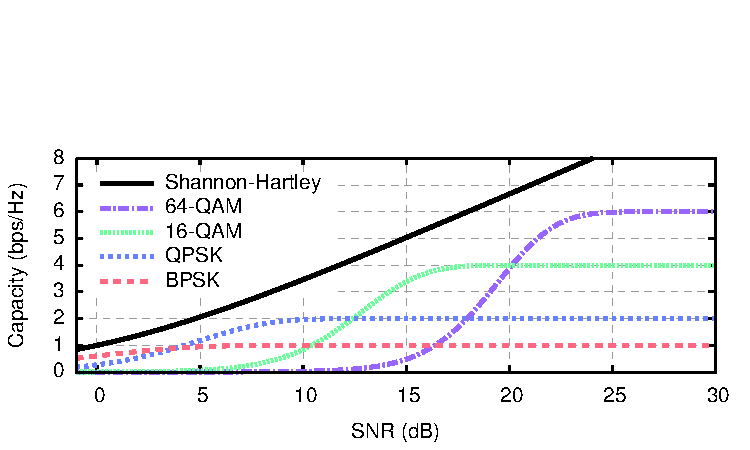
\includegraphics{calculations/snr_bits}
\caption[Capacity vs SNR for 802.11n modulation and coding schemes]{\label{fig:mod_bits_snr}The relationship between SNR and capacity for standard modulation schemes and idealized codes.}
\end{figure}

This property of the performance of different modulation schemes is closely related to the Shannon Capacity. \figref{fig:mod_ber_snr} illustrates the magnitude of this effect for the modulations used by 802.11 using textbook formulas~\cite{Sklar} that relate the SNR to a bit error rate. We can also connect these different modulations directly to the Shannon-Hartley Capacity Theorem by examining the capacity achieved by each scheme as a function of SNR (\figref{fig:mod_bits_snr}). In this graph, I assume an idealized coding scheme that delivers the maximum data rate for a given bit error rate; the practical schemes in widespread use today are somewhat less efficient in order to admit less expensive computation.\footnote{Though beyond the scope of this thesis, a number of recent proposals for practical \define{rateless codes}~\cite{Gudipati_Strider,Perry_Spinal} nearly achieve the Shannon Capacity bound by using much denser constellations and clever coding schemes across multiple transmissions.}

\subsection{The Wireless Channel}
The previous section explained the basics of digital communications in the context of a wired link. Here, I expand to the significantly more complex case of a wireless channel.

In a wireless link, the electromagnetic signal is emitted from an antenna as a \define{radio wave} that then radiates through the \define{wireless medium}, i.e.\ the environment. The dominant source of attenuation in an wireless link is not absorption by the medium, but rather the diffusion of energy throughout the environment, of which a small fraction is captured by a receiver's antenna. This effect, called \define{path loss}, is captured by the Friis transmission equation, which yields the inverse relationship
\begin{equation}
\label{eq:friis}
	S \propto \frac{T}{d^n},
\end{equation}
where $d$ is the distance between transmitter and receiver, and $n$ is the path loss exponent. In free space, $n$ has a value of 2, reflecting the fact that the energy transmitted at a particular time is spread out over the two-dimensional surface of a sphere, an area that grows with $d^2$. (For a directional antenna, the energy is spread over a different geometric shape, e.g. a cone, but this shape will still have a two-dimensional surface area).

The path loss exponent varies in different indoor environments, but empirically tends to take on a value between 2 and 4~\cite{Sklar}. This empirical result is explained as the sum of many complex effects that result from the interaction of radio waves with objects in the environment. One such effect is \define{shadowing}, in which materials such as glass or metal prevent radio waves from passing through. I explain more additional, more complicated channel effects below.

In wireless systems, multiple devices might send at the same time and in the same frequency band; this \define{interference} causes a \define{collision} during which a receiver will measure the sum of both transmissions. There are a number of practical problems for operation during a collision, such as whether the receiver can properly lock onto the desired signal and estimate the effects of the channel on it. In general, however, we can model the reception probability by replacing the SNR with the \define{signal-to-interference-and-noise ratio (SINR)}, which treats the interfering signal of power $I$ as another source of noise:
\begin{equation}
\label{eq:sinr}
\rho_I = \frac{S}{I+N}.
\end{equation}
While interference is an important problem, many systems, including 802.11, use \define{medium access control (MAC)} protocols to ensure that at most one device transmit at a time.

Beyond path loss, the most important channel effect is the inherent \emph{multi-path} nature of indoor wireless environments. At 2.4\GHz and 5\GHz, RF signals bounce off metal and glass surfaces that are common indoors. This scattering leads to a situation in which many copies of the signal arrive at the receiver having traveled along many different paths. The net effect of this RF superposition depends on the phases of the individual signals. When these copies combine they may add constructively, giving a good overall signal, or destructively, mostly canceling the overall signal.

The phase-dependent nature of multi-path effects means that they vary over both frequency and space. For a given distance traveled $d$, the phase change is $2\pi d/\lambda$. Thus wideband channels may exhibit dramatically different received power levels for different frequencies; such channels are called \define{frequency selective}. Measurement studies of frequency-selective fading report signal variations as high as 15--20\dB~\cite{Judd_CHARM}; in \chapref{chap:problem} I will present experimental evidence confirming these effects in the environments I studied.

With regard to spatial variation, the small 12\cm and 6\cm wavelengths of Wi-Fi signals means that small changes in path lengths can alter a situation from good to bad. Statistical models tell us that multi-path fading effects are independent for locations separated by as little as half a wavelength. This means that multi-path causes rapid signal changes or fast fading as the receiver moves, or in the case of a stationary node as the surrounding environment changes.  Movement at fast speed also induces \define{Doppler effect}, which aggravates multi-path effects and makes the channel even more variable.
%This means that some unlucky frequencies in a wide channel may be wiped out while others are unaffected.

The net effect of multi-path fading is that the received wireless signal can vary significantly over time, frequency and space. This is a problem for good performance because at any given time there is a significant probability of a deep fade that will reduce the SNR of the channel below the level needed for a given communication scheme.

However, an alternative way of looking at the effects of multi-path fading is that they provide \define{diversity}. In a sufficiently rich multi-path environment, there are so many combining copies of signals that the channel observed on different, nearby frequencies can be considered to be independently faded. For this reason among others, many systems including 802.11 use a scheme called Orthogonal Frequency Division Multiplexing (OFDM). In OFDM, a wide frequency band is split into many \define{subcarriers} that each carry different modulated bits in parallel, with a higher level error-correcting code across them to take advantage of this \define{frequency diversity}.

To get fast rates while only using sending a single symbol at a time, a wideband system must have a fast symbol rate. Since OFDM sends many symbols in parallel on smaller subcarriers, an OFDM system sends each symbol for a longer period of time. Thus by turning a single fast channel into many parallel slower channels, OFDM allows more time for the channel to average out temporal fades and provides \define{time diversity}.

One more type of diversity is \emph{spatial diversity}: antennas separated by at least half a wavelength see independently-faded channels. Devices with multiple antennas can use schemes that take advantage of the spatial diversity these antennas provide. For example, a multi-antenna receiver measures multiple independent copies of each transmitted signal. Thus with clever signal processing, such a receiver can align the phases of these copies and add them together, which averages out the noise and improves overall channel performance. In a complementary manner, a multi-antenna transmitter with knowledge of the fading properties of the individual paths between pairs of antennas can steer its signal such that the multiple copies arriving at the receiver's antenna combine optimally. This process, in which the gain and phase of the signal emitted by each antenna are adjusted (with OFDM, this adjustment may be different for each subcarrier) is called \define{beamforming}.
%A different technique called \define{space-time codes} to achieve the same effect, but 

Finally, suppose that both the transmitter and receiver have multiple antennas. The foundational work by Foschini, Gans~\cite{Foschini_Gans} and Telatar~\cite{Telatar_MIMO} in the mid 1990s introduced \define{spatial multiplexing}, which uses this new spatial degree of freedom to improve capacity. Instead of sending the same data out each antenna as above, a transmitter with $M$ antennas can use its different antennas to send up to $M$ independent \define{spatial streams} of data. An $N$-antenna receiver will then measure $N$ copies of each stream, each antenna an independent linear combination of the $M$ transmitted streams. If $M \leq N$, the receiver has enough information to solve the linear system and separate the streams, thus providing an $M$-fold gain in performance. Thus spatial multiplexing, with $N$ antennas at each side, results in a modified capacity theorem:
\begin{equation}
\label{eq:mimo_capacity}
R = BN\log_2(1+\rho).
\end{equation}
Together, spatial diversity and spatial multiplexing techniques form a set of what are called MIMO (multiple-input, multiple-output) techniques.

I conclude this discussion by mentioning one last channel effect relevant to 802.11: \define{inter-symbol interference}. In multi-path environments, some spatial paths can be so long that the delayed copies of the signal substantially overlap with the next symbol and make it harder to receive. The delay between the earliest and latest copies is called the \define{delay spread} of the channel, and it can be substantial. OFDM systems that use longer symbol times are more resilient to this effect, but still repeat each symbol for a period of time called a \define{guard interval}. If the guard interval is at least as long as the delay spread, the receiver can ignore the inter-symbol interference and still receive a complete symbol.

%For a variety of practical reasons, but in large part to combat multi-path fading, many modern protocols use .
%In 802.11, the 20\MHz-wide channel is broken into 64 \define{subcarriers}, each using 312.5\kHz of bandwidth.
%The beauty of OFDM is that it divides the channel in a way that is both computationally and spectrally efficient. High aggregate data rates can be achieved, while the encoding and decoding on different subcarriers can use shared hardware components.
%The individual subcarriers yield relatively independently faded channels (because of multi-path fading), and hence provide \define{frequency diversity} that is realized by coding across them.

%Dividing the channel also increases the symbol time per channel, since many slow symbols are sent in parallel instead of many fast symbols in sequence. This adds \define{time diversity} because the channel is more likely to average out fades over a longer period of time. Additionally, OFDM links compensate for multi-path by 
%In 802.11, which is targeted for roughly 100\m links, a secondary path might travel 200\m before reflecting, delayed by 667\ns from a pure line-of-sight path; 802.11 uses an 800\ns guard interval to compensate.  

%\begin{itemize}
%\item Fading, multipath, Doppler, etc. All of the above describe how we can get capacity out of the wireless channel. The hard part, and what most of all Wi-Fi research centers around, is how we develop protocols and systems to realize this capacity in the face of these effects.

%\item Collisions and SINR.

%\end{itemize}

\subsection{Summary}
\label{sec:background_80211n}
In this section, I have presented the fundamental principles of digital communication of wired and wireless channels, including the limits of noisy RF channels and how data is encoded. I have also described the most relevant channel effects that communicating devices must overcome, and the primary techniques used to do so. In the next section, I make this discussion concrete in the context of Wi-Fi by describing the specifics of the IEEE 802.11n standard. 

\section{The IEEE 802.11n Standard}
The IEEE 802.11 (Wi-Fi) standard~\cite{80211} is targeted towards defining a mode of operation for a \define{wireless local area network (WLAN)}, intended to provide medium-range connectivity ($\approx$100\m) using low transmit power (at most 1\W). It was first introduced in 1997, and has been amended many times since. In this thesis, I limit my discussion to the features of 802.11n, the newest physical layer amendment, and 802.11a, its predecessor.

Wi-Fi devices use unlicensed spectrum in the 2.4\GHz and 5\GHz bands, and must coexist with consumer electronics such as microwaves, cordless phones, and baby monitors. In addition to this cross-device interference, nearby Wi-Fi networks in separate administrative domains---such as neighboring apartments---may need to share the same channel. As a result, Wi-Fi networks are not planned in a centralized fashion, but rather use decentralized protocols that work towards a good solution in a distributed fashion. For instance, 802.11 includes a \define{carrier-sense multiple access (CSMA)} protocol to manage which devices send: in essence, a transmitter listens to ensure no other devices are transmitting before sending a packet, and reduces its sending probability exponentially (via \define{exponential backoff}) if its transmission is not acknowledged.

At the physical layer, 802.11 uses the modulation schemes and OFDM I described above, operating over 20\MHz channels. In conjunction with different modulations, 802.11 also uses error-correcting codes with different \define{coding rates} to achieve different operating points in the rate-robustness tradeoff space. I summarize the specific single-stream configurations in 802.11n as well as the resulting link data rates in \tabref{tab:siso_mcs}.

\begin{table}[t]
\centering
%\footnotesize
\begin{tabular}{cccc}
\toprule
MCS & Modulation & Coding Rate & Data Rate (Mbps) \\
\midrule
0 & BPSK & 1/2 & 6.5 \\
1 & QPSK & 1/2 & 13.0\\
2 & QPSK & 3/4 & 19.5\\
3 & 16-QAM & 1/2 & 26.0\\
4 & 16-QAM & 3/4 & 39.0\\
5 & 64-QAM & 2/3 & 52.0\\
6 & 64-QAM & 3/4 & 58.5\\
7 & 64-QAM & 5/6 & 65.0\\
\bottomrule
\end{tabular}
\caption[The 802.11n single-stream rates]{\label{tab:siso_mcs} The single-stream 802.11n modulation and coding schemes (MCS). These are only slightly different than the 802.11a MCS that achieved up to 54\Mbps. The increase in maximum rate comes from slightly more efficient use of OFDM subcarriers and a new, less redundant 5/6-rate code.}
\end{table}

The standard link metric is the \define{receive signal strength indicator (RSSI)}. The RSSI was included in the 802.11 standard from the beginning as ``a measure by the [physical layer hardware] of the energy observed at the antenna used to receive the current [packet]''~\cite[\S 17.2.3.2]{80211}. There are no specified requirements on its accuracy, instead, it is only required to be ``a monotonically increasing function of the received power''~\cite[\S 17.2.3.2]{80211}, and is generally used by the hardware to tell whether another device is transmitting. In practice, however, the RSSI reported by commercial Wi-Fi chipsets is an estimate of the received signal power and can be meaningfully translated into units of dBm. In this case, RSSI can be used in combination with noise measurements to compute the SNR of the link.

The 2009 standard amendment to IEEE 802.11n~\cite{80211n} added functionality and protocols for multi-antenna techniques such as spatial diversity, spatial multiplexing, and beamforming. The 802.11n enhancements are shown in \tabref{tab:11n_enhancements}. Most of improvement in the maximum data rate---from 54\Mbps in 802.11a to 600\Mbps in 802.11n---comes from the ability to use wider channels and multiple spatial streams. Together, these add $2\cdot2\cdot4=16$ times as many configurations to the space of a single link. Beamforming is effectively an analog parameter and adds nearly unbounded options.\footnote{For transmitter and receiver each using 4 antennas on a 40\MHz channel, representing the beamforming matrices at maximal resolution takes 29,184 bits.} The gains of beamforming vary depending on the channel---for strong links, they tend to be small, but for weak links they can provide dramatic performance improvements~\cite{Atheros_11nTechPaper}.

\begin{table}[t]
\centering
%\footnotesize
\begin{tabular}{lcp{3.1in}}
\toprule
Enhancement & Capacity Gain & Description \\
\midrule
Short OFDM & \multirow{2}{*}{$1.11\times$} & Data can be more efficiently encoded when the \\
guard interval & & multi-path delay spread is low.\\
\multirow{2}{*}{Spatial multiplexing} & \multirow{2}{*}{$2\times$ to $4\times$} & \multirow{2}{*}{Up to 4 concurrent spatial streams.} \\
\vspace{-6pt}\\
\multirow{2}{*}{40\MHz channels} & \multirow{2}{*}{$2.08\times$} & \multirow{2}{*}{More bandwidth, higher capacity (\sheqref{eq:shannon_capacity}).} \\
\\
\multirow{3}{*}{Beamforming} & \multirow{3}{*}{??} & A sender with multiple transmit antennas can shape its signal to match the RF channel, improving both performance and reliability. \\
\bottomrule
\end{tabular}
\caption[The 802.11n physical layer enhancements]{\label{tab:11n_enhancements} IEEE~802.11n adds a number of enhancements to the base single-stream configurations depicted in \tabref{tab:siso_mcs}. The performance improvement from beamforming varies depending on the properties of the wireless channel.}
\end{table}

The hardware/software interface in 802.11n operates at the level of individual packets or continuously-transmitted batches of packets. Packets are sent to the hardware and transmitted over the air. The receiver detects a new transmission from the increase in energy, estimates the parameters of the wireless channel from the packet's standard, known preamble, and then decodes the packet. The standard behavior for 802.11 links is that all bits---after error correction---must be correct in order for a packet to be received, otherwise the packet is dropped by the hardware. Correctly received packets are delivered to the software layer in conjunction with physical layer configuration information about the transmission (e.g., what MCS in \tabref{tab:siso_mcs} was used) and reception (e.g., which receive antennas were used) of the packet, plus physical layer metrics of link quality.

\section{Summary}
In this chapter, I have presented the background information to provide a basic understanding of wireless channels and the specific IEEE 802.11n technology used to operate in them. As I described in \secref{sec:background_80211n}, there are many different techniques that a transmitter and/or receiver can use to achieve robust operation in indoor wireless channels. However, the challenge---and the focus of most Wi-Fi research---is to decide which techniques to use, when to use them, and how to configure them to obtain the best operating point given the actual properties of the wireless channel. This is the primary problem I tackle in this thesis; in the next chapter I describe this problem in detail and given an overview of my approach.

%%%%%%%%%%%%%%%%%%%%%%%%%%%%%%%%%%
\ifx\mainfile\undefined
%
% ==========   Bibliography   ==========
%
%\nocite{*}   % include everything in the uwthesis.bib file
\bibliographystyle{plain}
\bibliography{dhalperi_thesis}

\end{document}
\fi

\ifx\mainfile\undefined
%  ========================================================================
%  Copyright (c) 2006-2011 The University of Washington
%
%  Licensed under the Apache License, Version 2.0 (the "License");
%  you may not use this file except in compliance with the License.
%  You may obtain a copy of the License at
%
%      http://www.apache.org/licenses/LICENSE-2.0
%
%  Unless required by applicable law or agreed to in writing, software
%  distributed under the License is distributed on an "AS IS" BASIS,
%  WITHOUT WARRANTIES OR CONDITIONS OF ANY KIND, either express or implied.
%  See the License for the specific language governing permissions and
%  limitations under the License.
%  ========================================================================
%
 
\documentclass [11pt, twoside] {uwthesis}

\usepackage{color}
\usepackage{url}
\usepackage{amsmath}
\usepackage{amsfonts}
\usepackage[bookmarks,
	hidelinks,
	plainpages=false,
	pdfpagelabels,
	pagebackref=true,
            ]{hyperref}
\renewcommand*{\backref}[1]{}% for backref < 1.33 necessary
\renewcommand*{\backrefalt}[4]{%
  \ifcase #1 %
    (No citations.)%
  \or
    (Cited on page #2.)%
  \else
    (Cited on pages #2.)%
  \fi
}

\newcommand{\biburl}[1]{{\tt<}\url{#1}{\tt>}}

\hypersetup{%
pdfauthor = {Daniel Chaim Halperin},
pdftitle = {Simplifying the Configuration of 802.11 Wireless Networks with Effective SNR},
pdfsubject = {Ph.D. Dissertation},
pdfkeywords = {},
pdfcreator = {University of Washington, Computer Science and Engineering},
pdfproducer = {},
bookmarksopen = {true},
pdfpagelayout = {TwoColumnRight},
}

\usepackage{footnotebackref}
%%%%%%%%%%%%%%%%%%%%%%%%%%%%%%%%%%%%%%%%%%%%%%%%%%%%%%
%%%        Formatting sections                     %%%
%%%%%%%%%%%%%%%%%%%%%%%%%%%%%%%%%%%%%%%%%%%%%%%%%%%%%%
\newcommand{\algref}[1]{Algorithm~\ref{#1}}
\newcommand{\chapref}[1]{Chapter~\ref{#1}}
\renewcommand{\eqref}[1]{Equation~\ref{#1}}
\newcommand{\figref}[1]{Figure~\ref{#1}}
\newcommand{\secref}[1]{\S\ref{#1}}
\newcommand{\tabref}[1]{Table~\ref{#1}}
\newcommand{\heading}[1]{\vspace{4pt}\noindent\textbf{#1}}
\newcommand{\topheading}[1]{\noindent\textbf{#1}}
\newcommand{\noheading}[0]{\vspace{4pt}\noindent}

%%%%%%%%%%%%%%%%%%%%%%%%%%%%%%%%%%%%%%%%%%%%%%%%%%%%%%
%%%        XXX and other warnings                  %%%
%%%%%%%%%%%%%%%%%%%%%%%%%%%%%%%%%%%%%%%%%%%%%%%%%%%%%%
\newcommand{\xxx}[1]{\textit{\color{red}XXX #1}}

%%%%%%%%%%%%%%%%%%%%%%%%%%%%%%%%%%%%%%%%%%%%%%%%%%%%%%
%%%        Units                                   %%%
%%%%%%%%%%%%%%%%%%%%%%%%%%%%%%%%%%%%%%%%%%%%%%%%%%%%%%
\usepackage{xspace}
\newcommand{\unitsep}{\texorpdfstring{\,}{ }}
\def\unit#1{% from: http://www.tex.ac.uk/cgi-bin/texfaq2html?label=csname "Defining a macro from an argument"
  \expandafter\def\csname #1\endcsname{\unitsep\text{#1}\xspace}%
}
\def\varunit#1#2{% from: http://www.tex.ac.uk/cgi-bin/texfaq2html?label=csname "Defining a macro from an argument"
  \expandafter\def\csname #1\endcsname{\unitsep\text{#2}\xspace}%
}
\unit{GHz}
\unit{MHz}
\unit{kHz}
\unit{Gbps}
\unit{Mbps}
\unit{KB}
\unit{dB}
\unit{dBi}
\unit{dBm}
\unit{W}
\unit{mW}
\varunit{uW}{$\mu$W}
\unit{ms}
\varunit{us}{$\mu$s}
\unit{h}
\unit{m}
\unit{s}
\unit{km}
\unit{cm}
\unit{mm}
\varunit{mmsq}{mm$^\text{2}$}
\varunit{insq}{in$^\text{2}$}
\newcommand{\degree}{\ensuremath{^\circ}\xspace}
\newcommand{\degrees}{\degree}
%%%%%%%%%%%%%%%%%%%%%%%%%%%%%%%%%%%%%%%%%%%%%%%%%%%%%%%%%%%%%%%%%%%%%%%%%%%%%%%%%%%%%%
% Euler for math | Palatino for rm | Helvetica for ss | Courier for tt
%
% From: http://www.tug.org/mactex/fonts/LaTeX_Preamble-Font_Choices.html
%%%%%%%%%%%%%%%%%%%%%%%%%%%%%%%%%%%%%%%%%%%%%%%%%%%%%%%%%%%%%%%%%%%%%%%%%%%%%%%%%%%%%%
\renewcommand{\rmdefault}{ppl} % rm
\usepackage[scaled]{helvet} % ss
\usepackage{courier} % tt
\usepackage{eulervm} % a better implementation of the euler package (not in gwTeX)
\normalfont
\usepackage[T1]{fontenc}
%%%%%%%%%%%%%%%%%%%%%%%%%%%%%%%%%%%%%%%%%%%%%%%%%%%%%%%%%%%%%%%%%%%%%%%%%%%%%%%%%%%%%%

%%%%%%%%%%%%%%%%%%%%%%%%%%%%%%%%%%%%%%%%%%%%%%%%%%%%%%
%%%        Figures                                 %%%
%%%%%%%%%%%%%%%%%%%%%%%%%%%%%%%%%%%%%%%%%%%%%%%%%%%%%%
\usepackage{graphicx}
% Caption package both lets you set the spacing between figure and caption
% and also makes the \figref{} point to the right place.
\usepackage[font=bf,aboveskip=6pt,belowskip=-4mm]{caption}
% Allow subfigures, make them bold
\usepackage[bf,BF,small]{subfigure}
% List of figures
\setcounter{lofdepth}{2}  % Print the chapter and sections to the lot

%%%%%%%%%%%%%%%%%%%%%%%%%%%%%%%%%%%%%%%%%%%%%%%%%%%%%%
%%%        Lists with reduced spacing              %%%
%%%%%%%%%%%%%%%%%%%%%%%%%%%%%%%%%%%%%%%%%%%%%%%%%%%%%%
\usepackage{enumitem}

%%%%%%%%%%%%%%%%%%%%%%%%%%%%%%%%%%%%%%%%%%%%%%%%%%%%%%
%%%        Fancy tables                            %%%
%%%%%%%%%%%%%%%%%%%%%%%%%%%%%%%%%%%%%%%%%%%%%%%%%%%%%%
\usepackage{tabulary}
\usepackage{booktabs}

%%%%%%%%%%%%%%%%%%%%%%%%%%%%%%%%%%%%%%%%%%%%%%%%%%%%%%
%%%        Formatting techniques/tools/etc.        %%%
%%%%%%%%%%%%%%%%%%%%%%%%%%%%%%%%%%%%%%%%%%%%%%%%%%%%%%
\newcommand{\term}[1]{\texttt{#1}}

\begin{document}
 
\textpages
\setcounter{chapter}{2} % Set to n-1!
\fi
%%%%%%%%%%%%%%%%%%%%%%%%%%%%%%%%%%

\cleardoublepage
\chapter{Problem and Approach}
\label{chap:problem}
\label{chap:approach}

The problem I study in this thesis is how to inform configuration decisions for wireless networks. I begin this chapter by presenting some of the primary problems in this space.

Next, I discuss how we handle these challenges today. There are two primary classes of techniques: (1) \emph{statistics-based} schemes which only use packet reception or loss as a high-level indicator of channel performance, and (2) \emph{channel-based} schemes which use measurements of the RF channel to predict packet delivery. Generally, the former statistics are too specific, because a packet probe in one configuration says little about whether another configuration---say, at a different rate or antenna mode----will work similarly. The latter channel measurements are too general, because the data recorded today and the way they are applied only coarsely reflect the true behavior of wireless operation over the underlying RF channel.

I conclude this chapter by presenting the hypothesis of my research and my approach to demonstrating it. My hypothesis is that it is possible to unify wireless configuration decisions into a single framework that is simple and incurs little overhead, but still accurate. To do so, I develop a comprehensive system that uses low-level RF channel measurements in conjunction with a simple but powerful model that can predict the performance of every operating point in the entire configuration space. 

%According to the standards makers, one of the intended purposes of the RSSI is ``to aid in link optimization algorithms such as roaming decisions''~\cite[\S 19.9.5.10]{80211}.

%\section{Wireless Configuration Problems}
%In this section, I describe the configuration problems that arise in modern wireless links and wireless networks, made concrete in the context of multi-antenna 802.11n.
%
%%%%%%%%%%%%%%%%%%%%%%%%%%%%%%%%%%%%%%%%%%%%%%%%%%%%%%%%%%%%%%%%%%%%%%%%%%%%%%%%%%%%%%%%%%%%%%%%%%%%%%
\section{Problem: Rate Control for a Single Link}
\begin{figure}[t]
	\centering
	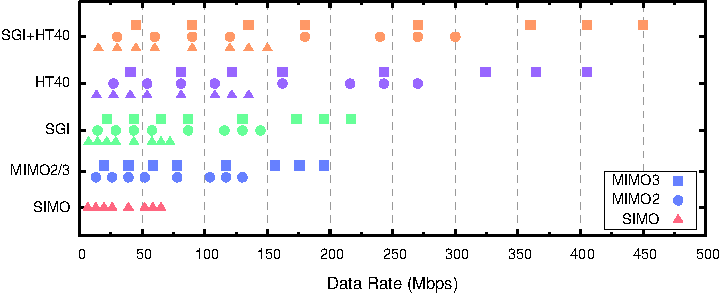
\includegraphics[width=\textwidth]{figures/rate_configs.pdf}
	\caption[The rate-related 802.11n configurations that use three antennas]{\label{fig:rate_configs}The different rate-related 802.11n configurations that use three antennas and 802.11n physical layer enhancements.}
\end{figure}

To accurately choose the rate at which to send data wirelessly, a rate control algorithm must find a good option among many possibilities. With 802.11n, which has adopted modern multi-antenna and physical layer techniques, this problem has gotten significantly more complex. To illustrate this, \figref{fig:rate_configs} shows the available rate configurations in 802.11n for a device with three antennas. These configurations use the eight modulation and coding scheme (MCS) combinations described in \tabref{tab:siso_mcs}, and the 802.11n enhancements shown in \tabref{tab:11n_enhancements}.

At the bottom of the figure, the SIMO line shows the eight single-stream configurations, which provide rates ranging from 6.5\Mbps to 65\Mbps. These are precisely the eight choices for rate that algorithms controlling a legacy 802.11a/g system must choose from.

In contrast, this space expands by a factor of 12 with 802.11n. Adding a second (MIMO2) and third (MIMO3) spatial stream increases the maximum rate to 195\Mbps, for a total of 24 different configurations. For each of these configurations, 802.11n adds the optional use of double-width (40\MHz, HT40) channels that raises the maximum rate to 405\Mbps with 48 choices. Finally, a physical layer tweak to a shorter OFDM guard interval (SGI) adds another $\approx 11\%$ and pushes the fastest configuration to 450\Mbps among 96 possibilities.

Looking forward, though three antennas are common today 802.11n can support up to four. The next amendment (802.11ac) will add two new single-stream rates using the 256-QAM modulation, plus channels of up to 160\MHz bandwidth. Combined, 802.11ac will comprise 320 configurations---a factor of 40 more than 802.11a. For the foreseeable future, the dramatic expansion in the rate space will continue as wireless technology improves.

Now having defined the basic problem of rate control, in the next two sections I describe the statistics-based and the channel-based approaches to solving it.

%%%%%%%%%%%%%%%%%%%%%%%%%%%%%%%%%%%%%%%%%%%%%%%%%%%%%%%%%%%%%%%%%%%%%%%%%%%
\section{Existing Statistics-based Approaches}
\begin{figure}[t]
      \centering
      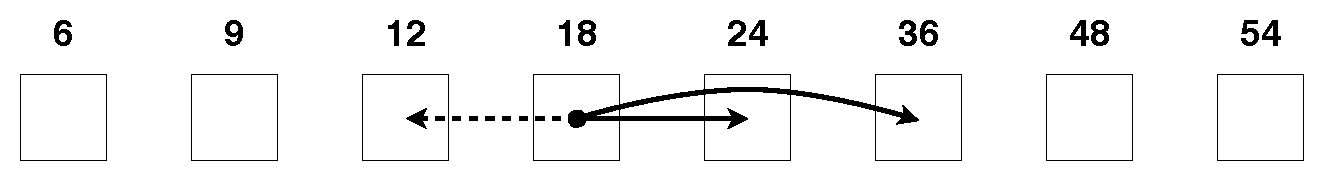
\includegraphics[scale=0.4]{figures/approach_figs/search_11a.pdf}
      \caption[Rate adaptation search pattern for 802.11a]{\label{fig:search_11a}A typical rate adaptation search pattern for 802.11a.}
\end{figure}
The majority of rate control algorithms today rely on packet loss statistics to adapt the operating rate. These algorithms use a large number of losses as a signal that the link quality is too poor to support the current rate, and hence fall back to a lower rate that is more easily received. Conversely, when a link experiences a very small number of losses using its current rate, it sends some \emph{packet probes} at a rate, and switches to the faster rate if it also works well. \figref{fig:search_11a} shows a typical 802.11a adaptation search pattern, where each box corresponds to an 802.11a rate and the arrows show the faster (solid) and slower (dashed) rates that might be probed.

The first algorithms (ARF~\cite{Kamerman_ARF} and AARF~\cite{Lacage_AARF}) would only switch between a rate and the next fastest or slowest; later implementations look up to two rates ahead~\cite{Bicket_SampleRate}. The dominant 802.11a rate adaptation algorithm used today is minstrel~\cite{minstrel}, which performs intelligent (biased) sampling of \emph{all} rates to keep up-to-date estimates of the global rate space and can thus take discontinuous jumps. Recent revisions to these algorithms have focused on better handling of corner cases, such as improving performance during hidden terminals via adaptive control over RTS/CTS~\cite{minstrel,Wong_RRAA}.

Some algorithms use bit error rate statistics instead of loss rate statistics to adapt rate. SoftRate~\cite{Vutukuru_SoftRate} estimates the bit error rate using a soft-output Viterbi decoder for error correction, and Chen et al.~\cite{Chen_EEC} designed a coding scheme called Error Estimating Coding (EEC) to enable accurate BER estimation at a higher layer.

\subsection{Complication: Multi-dimensional Search Space} 
%The explosion in the sheer number of configurations outlined in the prior section greatly complicates the rate configuration space for 802.11n, however this is only part of the problem.
All of the statistics-based approaches, which walk up or down the list of rates based on whether the current rate works well, implicitly rely on the following basic assumption (outlined by Vutukuru et al.~\cite{Vutukuru_SoftRate}):
\begin{center}
\textbf{Assumption:} \emph{BER is a monotonically increasing function of the bit rate.}
\end{center}
But 802.11n rate configurations are \emph{non-monotonic}. That is, it is not necessarily true that faster configurations are generally less likely to work than slower ones. This violates the axiom of these statistics-based approaches, and hence the \emph{multi-dimensional} search space must be treated as such. I explain why in the following example.

\figref{fig:rate_table_2d} shows three plausible \define{rate maps} for 3-antenna 802.11n links. In these rate maps, each row represents a different number of spatial streams, and each column represents a different MCS. A cell is shaded if a link can reliably deliver packets using that rate at that number of streams. The black box corresponds to \mcs{12}---2 streams at 39\Mbps each---which is the highest working 2-stream rate for these three hypothetical links.

\begin{figure}[t]
      \centering
      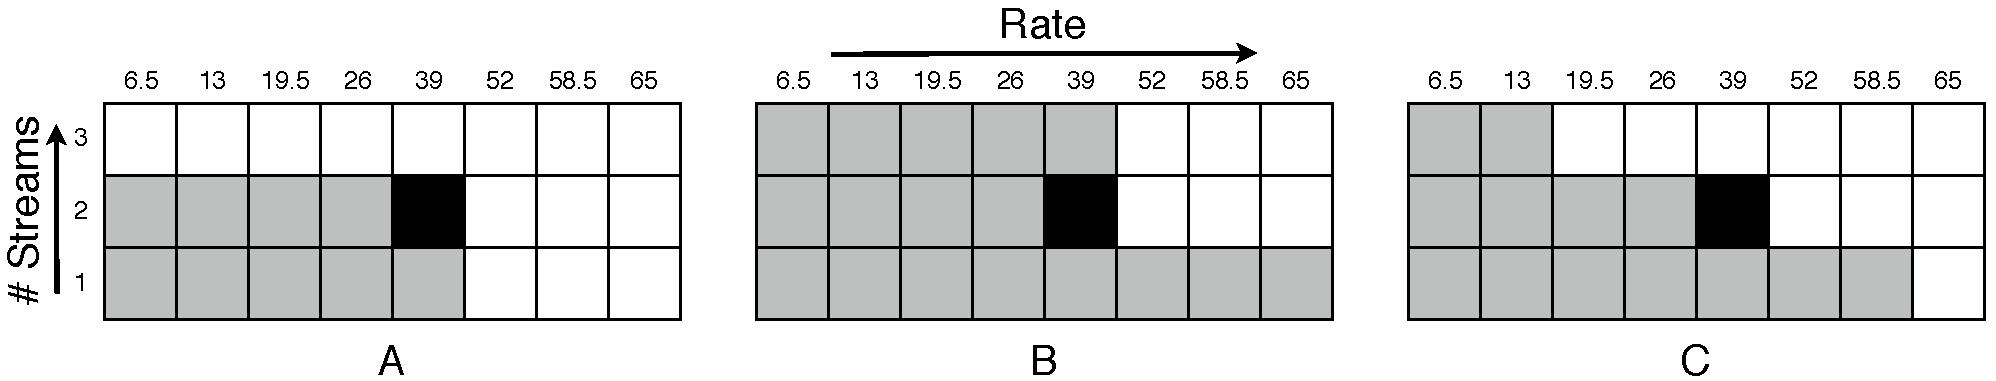
\includegraphics[width=\textwidth]{figures/rate_table_2d.pdf}
      \caption[Three different rate maps for 802.11n links]{\label{fig:rate_table_2d}Three different rate maps for 802.11n links. On these links, \mcs{12} (the black box) is the highest reliable 2-stream rate, and gray boxes indicate other reliable transmit configurations. A (\emph{left}): the worst possible situation in which no 3-stream rates and no higher single-stream configurations work. B (\emph{middle}): the best case in which all single stream rates work and all 3-stream rates work up to 39~Mbps each. C (\emph{right}): an average case in which the set of reliable rates decreases as more spatial streams are used.}
\end{figure}
\begin{figure}[t]
      \centering
      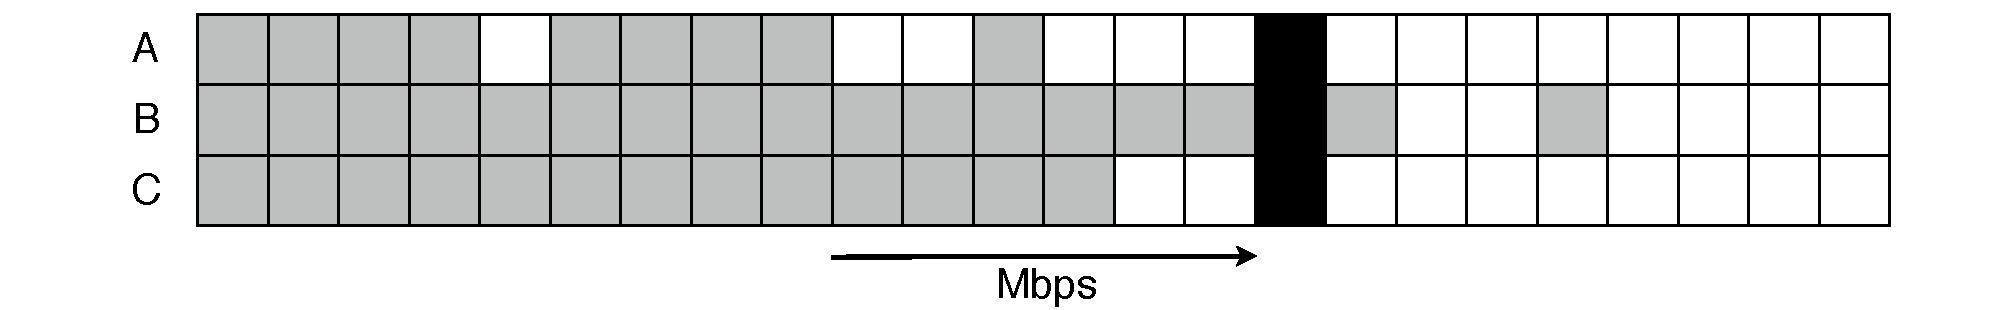
\includegraphics[width=\textwidth]{figures/rate_table_1d.pdf}
      \caption[Rate maps for the links in \figref{fig:rate_table_2d} mapped into one dimension]{\label{fig:rate_table_1d}Rate maps for the links in \figref{fig:rate_table_2d} now mapped into one dimension and sorted by total link speed (Mbps).
      %Ties (e.g., 1x39 and 3x13) are broken such that configurations with fewer streams come first.
      In this view, the strict monotonicity assumed by rate adaptation algorithms is violated, and the violations occur in a channel-dependent way. Thus, 802.11n rate adaptation requires optimization along multiple dimensions.}
\end{figure}

In 802.11n, each of the scenarios (A), (B), and (C) illustrated here is possible. In particular, if the link can reliably deliver packets using \mcs{12} then it is likely that \mcs{4}---the same encoding, but fewer streams---works as well. The same holds for \mcs{11}, since it uses the same number of streams but a less dense encoding. Similar logic implies all the shaded cells in link (A), which represents the most conservative situation in which \mcs{12} works well. Conversely, link (B) exhibits the best corresponding situation; higher-encoding single-stream configurations may also deliver most packets, and there may be little penalty from using 3 streams, thus resulting in the same set of 3-stream links working. Finally, link (C) exhibits an average case, in which lower rates must be used as the number of spatial streams increases.

The key is that each of these three links is plausible, which means that the search space for rate is non-monotonic in 802.11n. In \figref{fig:rate_table_1d}, I have redrawn the rate maps for these three links along a single-dimension, sorted by data rate. Ties in pure data rate---e.g., \mcs{1} vs \mcs{8}, both at 13\Mbps---are broken such that fewer streams is lower in the search. Here we can see that for all three links there exist higher rates that work well where lower rates do not. Thus a rate configuration algorithm for a multi-antenna link needs to consider a multi-dimensional search space.

\subsection{Current 802.11n Statistics-based Approaches}
\begin{figure}[t]
      \centering
      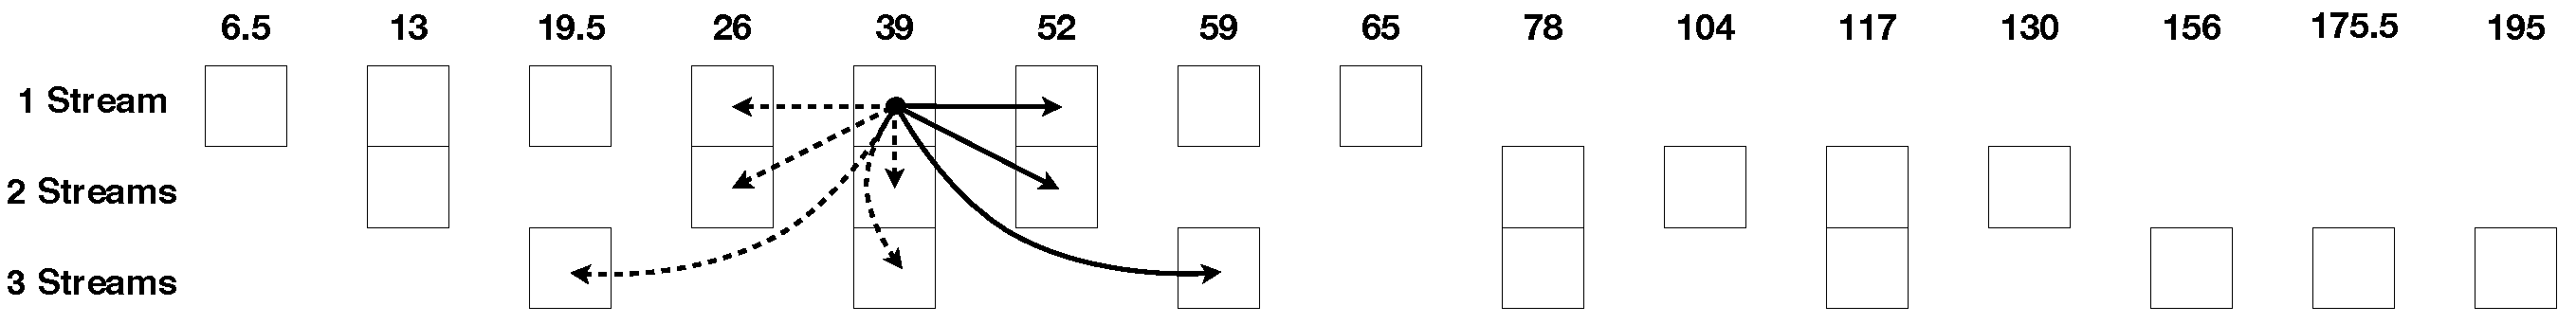
\includegraphics[width=\textwidth]{figures/approach_figs/search_11n.pdf}
      \caption[Rate adaptation search pattern for 802.11n]{\label{fig:search_11n}A typical rate adaptation search pattern for 802.11n.}
\end{figure}
\figref{fig:search_11n} illustrates the multi-dimensional search challenge with a concrete example. Each row corresponds to a transmit configuration with one, two, or three spatial streams. The eight boxes correspond to the eight 802.11n MCS combinations, placed in columns that reflect the aggregate link speed.

As we saw in \figref{fig:search_11a}, the single-dimensional search algorithm might try one or two rates higher, and during periods of loss it might fall back to the next lowest rate. In contrast, when increasing 802.11n rate from a single stream at \mcs{4} (39\Mbps), the configurations \mcs{5} (52\Mbps), \mcs{11} (MIMO2-52\Mbps), and \mcs{18} (MIMO3-58.5\Mbps) are all transmit configurations with better link speed, and each might work or not work depending on the channel. When \mcs{4} experiences loss, there are five choices of fallback configuration. This includes the higher-stream \mcs{10} (MIMO2-39\Mbps) and \mcs{17} (MIMO3-39\Mbps) which both have the same link speed and might work, as they use more robust modulation and coding combinations.

MiRA~\cite{Pefkianakis_MiRA} is a recent research algorithm that implements a version of this multi-probing scheme, as does the minstrel\_ht~\cite{minstrel_ht} algorithm used by the Linux kernel to do 802.11n rate selection in practice. A third approach is used by Intel's iwlwifi driver~\cite{iwlwifi}, which uses an 802.11a-like algorithm to select between MCS using a fixed number of streams, and adjusts the number of streams at coarse intervals.

\subsection{State of the Art in Statistics-based Approaches}
The dominant algorithms used in the Linux kernel today are minstrel~\cite{minstrel} (for 802.11a/g) and minstrel\_ht~\cite{minstrel_ht} (for 802.11n).  In general, statistics-based schemes provide good performance for static links in which the devices do not move and the surrounding environment does not change. For such cases, the algorithms may be inefficient at first but will converge to a good operating point. The challenge, as pointed out by several works~\cite{Holland_RBAR,Judd_CHARM,Vutukuru_SoftRate}, is that---depending on the speed at which devices move or the environment changes---these algorithms may be slow to react to varying conditions in mobile links environments, resulting in significant performance degradation.

SoftRate~\cite{Vutukuru_SoftRate} and EEC~\cite{Chen_EEC} are the newest BER-based adaptation algorithms. Both algorithms provide faster adaptation than their loss-based counterparts because by using the BER they can distinguish between a rate that is barely working with marginal BER (in which case the next fastest rate will not work) or has a lot of headroom (in which case it is worth probing the next fastest rate). These algorithms perform well at shifting up and down within a monotonic rate space; however, their BER estimations do not apply across the orthogonal dimensions such as multiple spatial streams. To handle 802.11n, these algorithms would need to be amended to do multi-dimensional search as well.

%%%%%%%%%%%%%%%%%%%%%%%%%%%%%%%%%%%%%%%%%%%%%%%%%%%%%%%%%%%%%%%%%%%%%%%%%%%%%%%%%%%%%%%%%%%%%%%%%%%%%%
\section{Channel-based Approaches}
The second class of approaches to configuring rate use channel information to guide rate selection or adaptation.
As I described in \chapref{chap:background} (\figref{fig:mod_ber_snr}), textbook analyses of modulation schemes give delivery probability for a single signal in terms of the signal-to-noise (SNR) ratio~\cite{Goldsmith}.
These theoretical models hold for narrowband channels with additive white Gaussian noise. They predict a sharp transition region of 1--2\dB over which a link changes from extremely lossy to highly reliable. This feature in theory makes the SNR a valuable indicator of performance.

This gives rise to a simple SNR-based configuration scheme, at least for selecting rate: Upon receiving a packet, a device can use the measured RSSI to compute the \define{Packet SNR} and predict the fastest rate supported. It can then feed this information back to the transmitter, which will use the newly selected rate for subsequent transmissions. This approach was explored in simulation by Holland et al.~\cite{Holland_RBAR} with an algorithm called RBAR, and shown to work well.

\subsection{Complication: Packet Delivery versus SNR in Practice}
Though SNR-based rate control algorithms may work well in simulation, subsequent practical work found that the Packet SNR computed from RSSI was unreliable~\cite{Aguayo_Roofnet, Reis_interference, Zhao_sensys03}. In very early devices, the RSSI was found to vary wildly over time or device temperature, providing unreliable thresholds; this was corrected by calibration in later devices (e.g., confirmed by Zhang et al.~\cite{Zhang_SNRguided} and by my measurements). Reis et al.~\cite{Reis_interference} found that RSSI estimates were corrupted by interfering transmissions. Finally, even in the absence of these latter effects, several studies found that the same RSSI value gives dramatically different performance for different links.

To understand which effects still hold for 802.11n hardware, I generated performance curves using an Intel Wireless Wi-Fi Link 5300 a/g/n (I describe my experimental platform in \chapref{chap:tool}) wireless network card. I connected two network cards together via a wire, and configured them to operate in a mode that uses a single antenna to transmit or receive. Using an inline variable attenuator I varied the amount of power received, and for each power level I sent around 1,000 packets using each of the eight 802.11n single-stream rates (\tabref{tab:siso_mcs}) and measured the fraction of delivered packets, the \define{packet reception ratio (PRR)}. With these measurements, I plotted the PRR against the link's SNR (computed from RSSI measurements at the receiver), and present the result in \figref{fig:snr_prr_attenuator}. 

\begin{figure}[t!]
	\centering
%	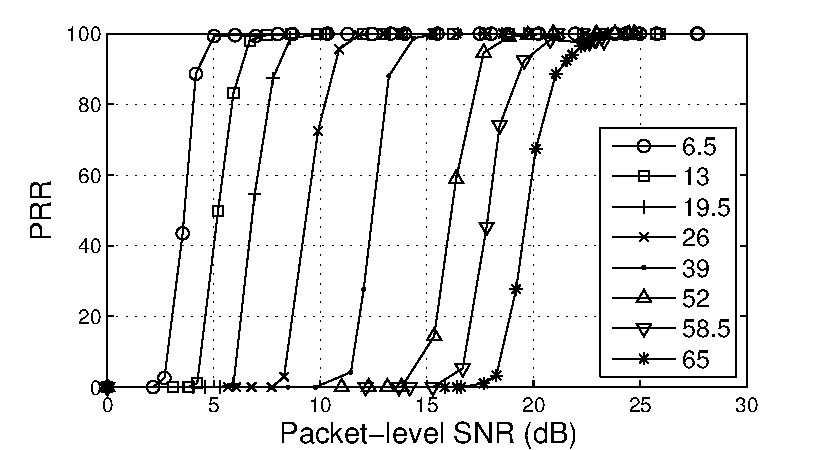
\includegraphics[width=\textwidth,viewport=13 0 364 204,clip]{figures/esnr/embed_attenuator_snr_prr.pdf}
	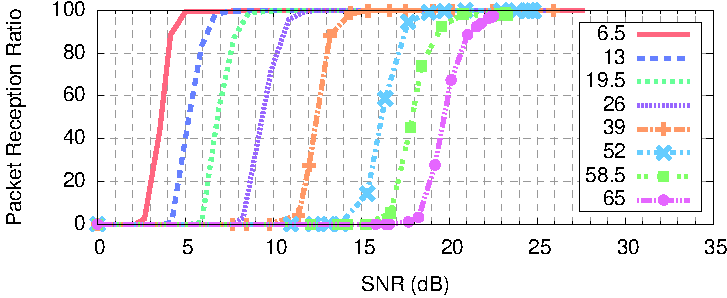
\includegraphics[width=\textwidth]{figures/snr_prr_atten.pdf}
	\caption[SNR vs PRR for a wired 802.11n link]{\label{fig:snr_prr_attenuator}A wired 802.11n link with variable attenuation has a predictable relationship between SNR and packet reception rate (PRR) and clear separation between rates.}
\end{figure}
\begin{figure}[t!]
	\centering
%	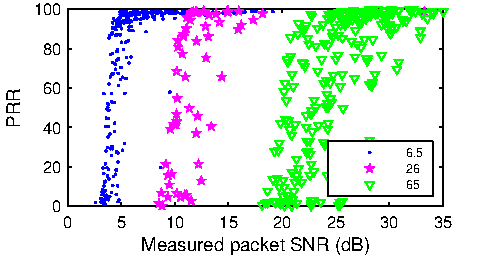
\includegraphics[width=\textwidth,viewport=2 0 217 124,clip]{figures/esnr/embed_scatterplot_meas_snr_small.pdf}
	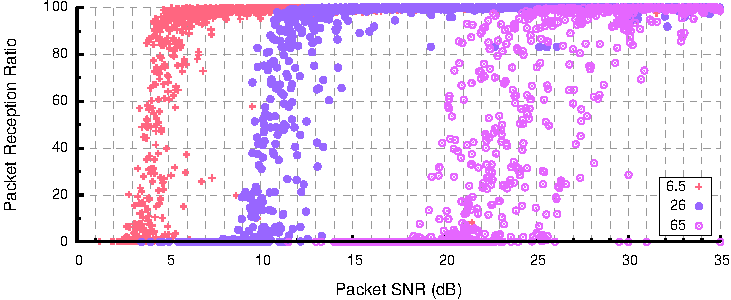
\includegraphics[width=\textwidth]{figures/snr_prr_scatter.pdf}
	\caption[SNR vs PRR for many wireless 802.11n channels]{\label{fig:snr_prr_26_65} Over real wireless channels in our testbeds, the transition region varies by 10\dB or more. The wireless channel loses the clear separation between rates (and so only three rates are shown for legibility).}%
\end{figure}

This figure shows a characteristic sharp transition region between SNR values at which the link goes from lossy to working, 2\dB at low modulations up to 4\dB for the fastest 65\Mbps rate. There is also a clear separation between rates: at a given SNR value, it is clear which rate should be used. This wired link provides a good approximation of a theoretical narrowband channel despite the relatively wide 20\MHz channel, the use of 56 OFDM subcarriers, coding and other bit-level operations. This is the behavior we would want from a link metric in order to predict packet delivery.

In contrast, packet delivery over real wireless channels does not exhibit the same picture. \figref{fig:snr_prr_26_65} shows the measured PRR versus SNR for three sample rates (6.5\Mbps, 26\Mbps, and 65\Mbps) over all wireless links in our testbeds, using the same 802.11n NICs. The SNR of the transition regions can exceed 10\dB, so that some links easily work for a given SNR and others do not. There is no longer clear separation between rates. This is consistent with the measurements from prior work mentioned above~\cite{Aguayo_Roofnet, Judd_CHARM, Reis_interference, Zhang_SNRguided, Zhao_sensys03}.

\subsection{State of the Art in SNR-based Approaches}
Although prior studies and my measurements showed that Packet SNR does not accurately predict delivery across links, they also found that for a particular link a higher SNR generally has higher packet delivery for a given rate~\cite{Aguayo_Roofnet,Judd_CHARM,Zhang_SNRguided}. Consequently, there are two algorithms, SGRA~\cite{Zhang_SNRguided} and CHARM~\cite{Judd_CHARM}, that use SNR feedback from the receiver in conjunction with packet loss statistics in order to learn the relationship between SNR and packet delivery online. Like statistics-based approaches, these algorithms work well for static links. Additionally, they provide good performance for fixed devices in mobile environments~\cite{Judd_CHARM}, because the learned relationship between SNR and PER is only slightly affected by moving objects and the learned calibration is generally valid. Successive measurements by Vutukuru et al.~\cite{Vutukuru_SoftRate} showed that CHARM tended to under-select in mobile links because it was unable to adapt its thresholds quickly enough to respond to the changing channel.

\subsection{Complication: High-level Measurement of Low-level Subchannel Effects}
I listed above several reasons that Packet SNR calculated from RSSI has historically been a poor predictor of performance. In the modern era of calibrated hardware, however, measurements no longer vary significantly with changing temperature or power level, or across devices. Instead, the dominant factor is likely to be the use of OFDM, and the presence of frequency-selective fading in the RF channel.

\begin{figure}[t]
  \centering
%  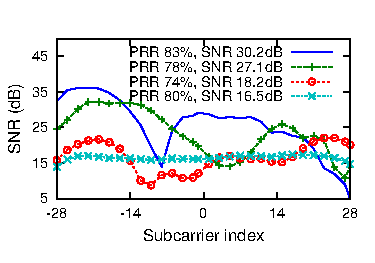
\includegraphics[width=\columnwidth,viewport=2 9 185 108,clip]{figures/esnr/embed_fsf-shape-two-links.pdf}
  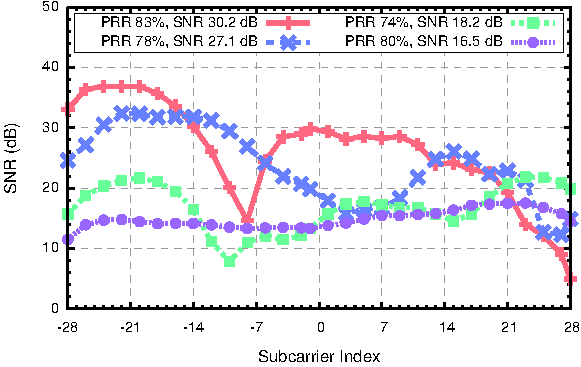
\includegraphics[width=0.8\textwidth]{figures/fsf_shape.pdf}
  \caption[Channel gains on four links that perform about equally well at 52\Mbps]{Channel gains on four links that perform about equally well at 52\Mbps. The more faded links require larger RSSIs (i.e., more transmit power) to achieve similar PRRs.}
  \label{fig:example_fsf_shape}
  % information for the links used to make above plot: 
  %srcs = [1 10 3 3];
  %dests = [9 11 2 5];
  %txpowers = [-4 20 28 20];

  % reference numbers from expt-8
  %prr = [80 83 78 74];
  %rss = [16.5 30.2 27.1 18.2];
\end{figure}

To illustrate this fact, I chose four representative links in my 802.11n testbed. These four links have SNRs ranging from 16\dB to 30\dB and yet they each perform similarly, delivering around 80\% of packets sent using single-stream \mcs{6} (52\Mbps). \figref{fig:example_fsf_shape} shows the packet reception rates and SNRs for these four links, but also includes the SNRs of the individual OFDM subcarriers for each links.

With this detailed picture, we can see that multipath causes some subcarriers to work markedly better than others although all use the same modulation and coding. These channel details, and not simply the overall signal strength as given by SNR, affect packet delivery. The fading profiles vary significantly across the four links. One distribution is quite flat across the subcarriers, while the other three exhibit frequency-selective fading of varying degrees. Two of the links have two deeply-faded subcarriers that are more than 20\dB down from the peak.

Because of these different fading profiles, these links harness the received power with different efficiencies.
The more faded links are more likely to have errors that must be repaired with coding, and require extra transmit power to compensate. Thus, while the performance is roughly the same, the most frequency-selective link needs a much higher overall packet SNR~(30.2\dB) than the frequency-flat link~(16.5\dB). This difference of almost 14\dB (more than $20\times$) highlights why Packet SNR based on RSSI does not reliably predict performance.

To exacerbate this issue, 802.11n adds MIMO techniques to the network. During a multi-stream transmission, the receiver still records only one RSSI value per antenna. This RSSI (and the resulting SNR) reflects the total received power combined across all subcarriers and all spatial streams. The total power received will vary with the number of streams, and the actual performance of the link will depend on how well this total power is balanced across spatial streams and how well the receiver can separate the two spatial streams. Thus in 802.11n Packet SNR is likely to be even less accurate when predicting link performance.

\subsection{Approach using Low-level RF Measurements}
\label{sec:accurate}
AccuRate~\cite{Sen_AccuRate} takes an alternative approach to using physical layer information to predict performance. Instead of measuring information about the \emph{signal power}, AccuRate measures the \emph{error vectors} (described in \chapref{chap:background}) of the received symbols when demodulating a packet. To make predictions about bit error rate, AccuRate then replays those same error vectors to a physical layer simulator, which models the reception of a packet using each of the different rates and selects the fastest successfully received packet. Though it would be impractical to implement a full physical layer simulator for each received packet, AccuRate was shown to be significantly more accurate than SNR-based algorithms with performance comparable to SoftRate. At the same time, AccuRate suffers from the same 802.11n-related flaws as the remaining algorithms: the magnitude of the error vectors will change depending on different numbers of spatial streams or channel widths or the use of a short guard interval, and AccuRate can handle none of these cases without implementing a multi-dimensional search.

%%%%%%%%%%%%%%%%%%%%%%%%%%%%%%%%%%%%%%%%%%%%%%%%%%%%%%%%%%%%%%%%%%%%%%%%%%%%%%%%%%%%%%%%%%%%%%%%%%%%%%
\section{Further Wireless Configuration Problems}
\label{sec:problems_11n}
In the previous section, I outlined the rate configuration problem, the current approaches, and the multi-dimensional aspects of OFDM and MIMO technologies that make them ineffective. In this section, I briefly mention many other problems and how they are solved in Wi-Fi networks today. (For a deeper discussion of each, see \chapref{chap:related}.) Together, these problems show the richness of the wireless network configuration space.

\subsection{Antenna Selection}
A transmitter sending fewer spatial streams than it has transmit antennas may wish to choose a subset of those antennas to save power or improve performance. Among production 802.11n drivers in Linux, only Intel~\cite{iwlwifi} has such an algorithm; within a fixed number of streams it occasionally probes the different transmit antenna configurations. In this algorithm, switching between transmit antenna sets occurs on timescales of seconds.

In the analogous scenario on the receive side, some chips automatically use only a subset of receive antennas when receiving a packet instead of fully maximizing available spatial diversity. These algorithms typically use Packet SNR measurements of the antennas to determine when additional antennas will add little gain. (Of course, this determination can be erroneous in the face of subchannel fading effects.)

\subsection{Channel Width Selection}
When both devices in an link support multiple channel widths, they may obtain better performance or power savings depending on the bandwidth they choose. SampleWidth~\cite{Chandra_SampleWidth} uses a probing algorithm to determine which width gives the best performance, aiming to achieve spectral isolation from interferers. For choosing between 20\MHz and 40\MHz bands, the algorithms in Linux tend to integrate channel width selection into the rate selection algorithm. When both widths are available, Intel's driver, which coarsely switches between different numbers of spatial streams, doubles the set of modes it probes by instantiating one copy for each potential bandwidth.

\subsection{Transmit Power Control}
Devices can adapt their transmit power levels to save energy or reduce interference with other nodes. In practice, however, all drivers seem to aim to optimize performance of their link. To that end, reducing transmit power can only reduce the maximum rate of the link and make interference worse by creating more hidden terminals; so this is never done in practice. Research proposals to achieve these ends typically rely on sampling performance and/or interference at various power levels.

\subsection{Access Point Selection}
When clients select which access point to connect to today, a number of factors are important, including both the quality of the link to the access point and also the load on that access point. Clients today typically choose access points solely based on the measured Packet SNR, on the assumption that it's a good proxy for downlink performance. Some proposed enterprise AP systems (e.g., DenseAP~\cite{Murty_DenseAP}) can take load into account as well.

One interesting note is that today's algorithms are not heterogeneity-aware. So given a choice of two APs: (1) with 30\dB SNR and 3 antennas, which would offer a rate of 250\Mbps, and (2) a closer AP with 35\dB SNR but only 2 antennas and supports only 100\Mbps, today's clients will still choose AP (2) with the larger SNR.

\subsection{Channel Selection}
Channel selection is the problem of choosing the best operating frequency for a pair (or set) of wireless devices. This is not a runtime choice in today's access point networks, because the frequency is chosen by the AP. However, this is likely to be a problem now that device-to-device connections are desirable in e.g., Wi-Fi Direct networks. (I note that algorithms have been proposed for the related problem of distributed access point channel assignment to manage load and interference~(e.g., \cite{Akella_Chan}).)

\subsection{Multi-Hop Routing}
Evaluating how well multi-hop paths through a wireless network is also irrelevant to today's AP networks. Most work in this space therefore applies to mesh networks, and usually uses a combination of probing, Packet SNR-based heuristics, and state space reduction (e.g, assuming single-antenna devices and a single fixed rate network-wide). One more practical recent proposal by Bahl et al.~\cite{Bahl_repeater} uses relays to address the rate anomaly problem in Wi-Fi access point networks, and uses Packet SNR to predict bitrate and calculate how well paths work. The performance of these solutions depends on the accuracy of these heuristics, which have not yet been adapted for heterogeneous devices or been made MIMO-aware.

\subsection{Spatial Reuse}
Spatial reuse is the problem of managing concurrent transmissions that occupy the same frequency. In today's access point networks, algorithms typically aim to have only one transmission at a time and adaptively turn on RTS/CTS when necessary to eliminate hidden terminals that hurt performance. A state-of-the-art algorithm to promote spatial reuse is CMAP~\cite{Vutukuru_CMAP}, which fixed the entire network to homogeneous single-antenna devices using the same rate and still required a complex distributed probing algorithm in a static environment to achieve good performance.

\subsection{Beamforming}
Finally, there is the problem of beamforming, that is, for a transmitter to shape the combined signal sent out its antennas so that the spatial paths best combine at the receiver. Theoretical gains from beamforming are evaluated by measuring the increase in Shannon capacity using ideal hardware and optimal receiver, rather than by the practical constraints of real hardware. I do not know of any practical systems for Wi-Fi that use this type of beamforming, but such a system would need a way to ground the output of the theoretical model to evaluate how the link would work in practice. Rather than an abstract complaint, there are real issues such as the tension between the optimal ``water-filling'' algorithms for beamforming~\cite{Tse} (which allocate power unequally across antennas or subcarriers) and practical hardware constraints such as amplifier peak-to-average-power limits.

In practice, I imagine that this grounding would be done by probing the link performance, as has been the case with analog beamforming strategies~\cite{Liu_DIRC} that operate in a fundamentally different way than 802.11n-like beamforming.

%%%%%%%%%%%%%%%%%%%%%%%%%%%%%%%%%%%%%%%%%%%%%%%%%%%%%%%%%%%%%%%%%%%%%%%%%%%%%%%%%%%%%%%%%%%%%%%%%%%%%%
\section{My Approach: an Effective SNR-based model for Wi-Fi}
My hypothesis is that \emph{it is possible to unify the decision-making components of wireless network configuration algorithms into a single comprehensive framework that is practical and provides good performance}. I envision a framework that is flexible enough to handle all the problems discussed in this section. To demonstrate this hypothesis, I develop a comprehensive system that uses low-level RF channel measurements in conjunction with a simple but powerful model that can predict the performance of every operating point in the entire configuration space. 

In particular, I develop a practical methodology that uses low-level measurements of the RF channel and the concept of an Effective SNR~\cite{Nanda_EffectiveSNR} to predict performance for wireless channels that use modern physical layer technologies such as OFDM, multiple antennas, variable channel widths, and spatial diversity and multiplexing. I also explain how to apply this prediction engine to a wide variety of link and network configuration problems such as those described in this chapter. To demonstrate that this methodology is practical, I prototype a working system in the context of IEEE 802.11n, which is the dominant consumer wireless networking technology today and includes these state-of-the-art RF techniques. Finally, to show that it works, I use my prototype to evaluate the accuracy of the choices made using my techniques. I find that my model accurately predicts packet delivery over hundreds of indoor wireless links in two environments, and that this level of accuracy is sufficient to lead to good configurations for many link and network problems.

\subsection{Effective SNR-based Model}
The central component in my thesis is a model for packet delivery that uses low-level RF measurements called CSI (see \secref{sec:csi} below) to predict packet loss over real wireless channels. To be useful, this model must accurately predict the packet delivery probability for a given physical layer configuration operating over a given channel. It must also simple and practical, so that it can be readily deployed, and cover a wide range of physical layer configurations, so that it can be applied in many settings and for many tasks.

In this thesis, I scope my model to devices that use MIMO and OFDM, which captures the fundamental technological primitives for many current and future networks. In particular, the scope of my model is 802.11n including all the enhancements described in \secref{sec:background_80211n}. My model is based on the concept of Effective $E_b/N_0$ developed by Nanda and Rege~\cite{Nanda_EffectiveSNR}, and described as follows.
 
\begin{figure}[t!]
	\centering
	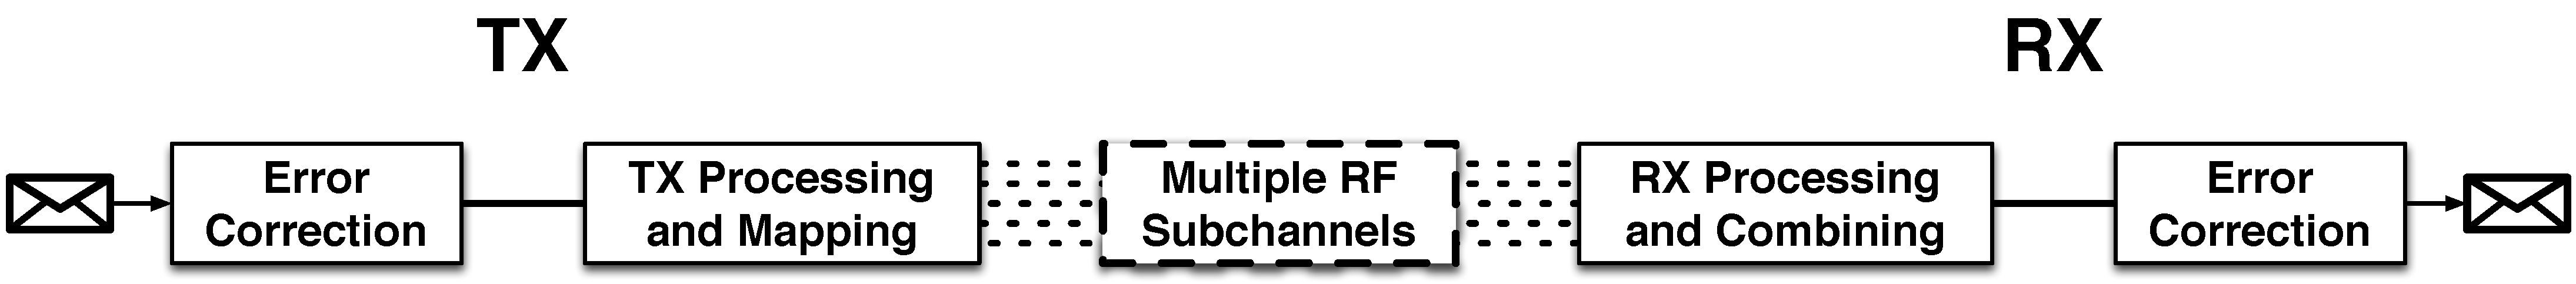
\includegraphics[width=\textwidth]{figures/esnr_intuitive.pdf}
	\caption[Simplified overview of an RF link operating over multiple subchannels]{\label{fig:esnr_intuitive}Simplified overview of an RF link operating over multiple subchannels.}
\end{figure}

\figref{fig:esnr_intuitive} shows a simplified overview of a link operating over an RF channel that has multiple subchannels, such as MIMO spatial paths or OFDM subcarriers. The transmitter applies error correction to the original data packet, and then processes the coded bitstream and maps the resulting symbols onto the multiple subchannels. The receiver processes the noisy signal to recover the (potentially errored) coded bitstream, and then uses error correction to attempt to recover the original data bits.

The key hypothesis introduced by Nanda and Rege is that error correction---in conjunction with mechanisms like frequency- and spatial-aware interleaving in 802.11n---works to spread the errors caused by faded subchannels across the entire channel. If this assumption holds, the link can be modeled as performing with an aggregate error rate equal to the average error rate across subchannels. This average bit error rate is called the \define{Effective BER} of the channel, and from it we can compute the \define{Effective SNR} of the channel. Since the four links displayed in \figref{fig:example_fsf_shape} have similar error performance, they should have similar Effective SNRs. Then the Effective SNR can be used as a metric of link quality, and hence provide accurate estimates of packet delivery.

\subsection{Model Input: Fine-grained RF Measurements}
\label{sec:csi}
As described above, the input to my Effective SNR-based system is a set of low-level RF channel measurements. The particular measurements I use in this thesis are called Channel State Information (CSI). For an OFDM link, the CSI comprises the channel gain coefficient (amplitude and phase,\footnote{Note that in \figref{fig:example_fsf_shape}, I plot only the amplitude as the phase offset does not affect packet delivery for a SISO link (assuming it is properly equalized by the receiver).} see \chapref{chap:background}) for each OFDM subcarrier. For an $N$x$M$ MIMO link, the CSI is an $N$x$M$ matrix where each entry reflects the channel gain coefficient from one transmit antenna to one receive antenna. For a MIMO-OFDM link such as in 802.11n, the CSI comprises a three-dimensional $N$x$M$x$S$ matrix that reflects the $N$x$M$ MIMO link for each of $S$ subcarriers.

A single comprehensive CSI measurement captures the low-level channel details that enable my model to calculate the Effective SNR for a wide configuration space. I next summarize how these measurements are used.

\subsection{Model Output, and how to Apply it}
I describe the model and how it's used in complete detail in the next chapter, but the basic structure of the model is simple: given (1) a current CSI measurement of the RF channel between transmitter and receiver, and (2) a target physical layer configuration of the transmit and receive NICs, it predicts whether that link will reliably deliver packets in that configuration.

With this simple decision primitive, we can easily build higher layer optimization protocols. These include solutions to all of the problems mentioned in this chapter, such as selecting the best rate, number of spatial streams, or transmit antenna set; whether to use 20\MHz or the entire 40\MHz channel; or choosing the lowest transmit power at which the link supports a particular rate.

Note that I do not try to make predictions in the transition region during which a link changes from lossy to reliable. Predictions there are likely to be variable, and simply knowing when the link starts to work is useful information in practice. For the model output, I define that the link will work, i.e., will reliably deliver packets, if the model predicts $\geq$90\% packet reception rate. As we will see in this thesis, this system provides good performance across a range of wireless configuration problems.


%steps are (1) comprehensively measuring CSI for the RF channel including all subchannels, (2) adapting that CSI measurement to model the transmit configuration problem under investigation, (3) modeling receiver behavior to come up with the post-processing SNRs of the individual subchannels, and (4) computing the bit error rates of the individual subchannels from their SNRs and then calculating the Effective BER and finally the Effective SNR.

\subsection{Problems Solved}
\begin{table}[htp]
	\centering
	\begin{tabular}{lc}
	\toprule
		\textbf{Application of Effective SNR} & \textbf{Described in} \\
	\midrule
		Bitrate/MCS selection & \chapref{chap:delivery}, \chapref{chap:rate}\\
		Channel width selection & \chapref{chap:delivery}, \chapref{chap:rate}\\
		Antenna selection & \chapref{chap:delivery}, \chapref{chap:rate}\\
		Transmit power control & \chapref{chap:delivery}\\
		Channel selection & \chapref{chap:applications}\\
		AP selection & \chapref{chap:applications}\\
		Path selection/BSS selection in WDS & \chapref{chap:applications}\\
		Interference planning/Spatial reuse \\
		Partial packet recovery/FEC & Bhartia et al.~\cite{Bhartia_FreqDiv}\\
		Beamforming \\
		Multicast rate selection \\
	\bottomrule
	\end{tabular}
	\caption[A variety of applications of Effective SNR]{\label{tab:esnr_uses}A variety of applications of Effective SNR\@.}
\end{table}

\tabref{tab:esnr_uses} shows a list of several potential applications of Effective SNR. These cover all the problems described above and range from optimizing various parameters of a single Wi-Fi link, such as the MCS or antenna set used, to coordinating many nodes in a dense wireless network. Additionally, I identify applications that can be implemented by looking at other aspects of the Channel State Information in \tabref{tab:csi_uses}. These provide useful primitives that can enable systems to adapt behavior based on the location and movement of the user.

Combined, I believe these form the critical building blocks for configuring dense future wireless networks like Wi-Fi Direct. In particular, my Effective SNR model provides the information needed to select rates or configure the network topology, among other things. The CSI can be used to supplement these schemes, particularly by using mobility classification to determine when a device starts to move and trigger reconfiguration of the wireless network in response. I implement and evaluate many of these applications in the rest of this thesis, several have been investigated by other researchers in follow-on work, and some are left for future research.

\begin{table}[tp]
	\centering
	\begin{tabular}{lc}
	\toprule
		\textbf{Application of CSI} & \textbf{Described in} \\
	\midrule
		Mobility classification & \chapref{chap:applications}\\
		Indoor localization & FILA~\cite{Wu_FILA}, PinLoc~\cite{Sen_PinLoc}, SpinLoc~\cite{Sen_SpinLoc} \\ 
	\bottomrule
	\end{tabular}
	\caption[A variety of applications of Channel State Information]{\label{tab:csi_uses}A variety of applications of Channel State Information.}
\end{table}

\section{Summary}
In this chapter I have presented a detailed overview of wireless link and network configuration problems, and the statistics-based and channel-based approaches we take to solving them today. Generally, statistics are too specific, applying only to a single or a few configurations. Conversely, channel measurements used previously have been too general, not capturing the low-level details of the channel. I then described my channel-based approach, which uses low-level channel measurements of the MIMO and OFDM subchannels in conjunction with an Effective SNR-based model to provide a way to predict performance over the broad configuration space. In the next chapter, I flesh out this model and how to use it, and argue that it is indeed flexible and has low overhead. In the remainder of the thesis, I will show that my model makes accurate predictions that lead to good choices of operating points in practice for many of the problems I described in this chapter.

%%%%%%%%%%%%%%%%%%%%%%%%%%%%%%%%%%
\ifx\mainfile\undefined
%
% ==========   Bibliography   ==========
%
%\nocite{*}   % include everything in the uwthesis.bib file
\bibliographystyle{plain}
\bibliography{dhalperi_thesis}

\end{document}
\fi

\ifx\mainfile\undefined
%  ========================================================================
%  Copyright (c) 2006-2011 The University of Washington
%
%  Licensed under the Apache License, Version 2.0 (the "License");
%  you may not use this file except in compliance with the License.
%  You may obtain a copy of the License at
%
%      http://www.apache.org/licenses/LICENSE-2.0
%
%  Unless required by applicable law or agreed to in writing, software
%  distributed under the License is distributed on an "AS IS" BASIS,
%  WITHOUT WARRANTIES OR CONDITIONS OF ANY KIND, either express or implied.
%  See the License for the specific language governing permissions and
%  limitations under the License.
%  ========================================================================
%
 
\documentclass [11pt, twoside] {uwthesis}

\usepackage{color}
\usepackage{url}
\usepackage{amsmath}
\usepackage{amsfonts}
\usepackage[bookmarks,
	hidelinks,
	plainpages=false,
	pdfpagelabels,
	pagebackref=true,
            ]{hyperref}
\renewcommand*{\backref}[1]{}% for backref < 1.33 necessary
\renewcommand*{\backrefalt}[4]{%
  \ifcase #1 %
    (No citations.)%
  \or
    (Cited on page #2.)%
  \else
    (Cited on pages #2.)%
  \fi
}

\newcommand{\biburl}[1]{{\tt<}\url{#1}{\tt>}}

\hypersetup{%
pdfauthor = {Daniel Chaim Halperin},
pdftitle = {Simplifying the Configuration of 802.11 Wireless Networks with Effective SNR},
pdfsubject = {Ph.D. Dissertation},
pdfkeywords = {},
pdfcreator = {University of Washington, Computer Science and Engineering},
pdfproducer = {},
bookmarksopen = {true},
pdfpagelayout = {TwoColumnRight},
}

\usepackage{footnotebackref}
%%%%%%%%%%%%%%%%%%%%%%%%%%%%%%%%%%%%%%%%%%%%%%%%%%%%%%
%%%        Formatting sections                     %%%
%%%%%%%%%%%%%%%%%%%%%%%%%%%%%%%%%%%%%%%%%%%%%%%%%%%%%%
\newcommand{\algref}[1]{Algorithm~\ref{#1}}
\newcommand{\chapref}[1]{Chapter~\ref{#1}}
\renewcommand{\eqref}[1]{Equation~\ref{#1}}
\newcommand{\figref}[1]{Figure~\ref{#1}}
\newcommand{\secref}[1]{\S\ref{#1}}
\newcommand{\tabref}[1]{Table~\ref{#1}}
\newcommand{\heading}[1]{\vspace{4pt}\noindent\textbf{#1}}
\newcommand{\topheading}[1]{\noindent\textbf{#1}}
\newcommand{\noheading}[0]{\vspace{4pt}\noindent}

%%%%%%%%%%%%%%%%%%%%%%%%%%%%%%%%%%%%%%%%%%%%%%%%%%%%%%
%%%        XXX and other warnings                  %%%
%%%%%%%%%%%%%%%%%%%%%%%%%%%%%%%%%%%%%%%%%%%%%%%%%%%%%%
\newcommand{\xxx}[1]{\textit{\color{red}XXX #1}}

%%%%%%%%%%%%%%%%%%%%%%%%%%%%%%%%%%%%%%%%%%%%%%%%%%%%%%
%%%        Units                                   %%%
%%%%%%%%%%%%%%%%%%%%%%%%%%%%%%%%%%%%%%%%%%%%%%%%%%%%%%
\usepackage{xspace}
\newcommand{\unitsep}{\texorpdfstring{\,}{ }}
\def\unit#1{% from: http://www.tex.ac.uk/cgi-bin/texfaq2html?label=csname "Defining a macro from an argument"
  \expandafter\def\csname #1\endcsname{\unitsep\text{#1}\xspace}%
}
\def\varunit#1#2{% from: http://www.tex.ac.uk/cgi-bin/texfaq2html?label=csname "Defining a macro from an argument"
  \expandafter\def\csname #1\endcsname{\unitsep\text{#2}\xspace}%
}
\unit{GHz}
\unit{MHz}
\unit{kHz}
\unit{Gbps}
\unit{Mbps}
\unit{KB}
\unit{dB}
\unit{dBi}
\unit{dBm}
\unit{W}
\unit{mW}
\varunit{uW}{$\mu$W}
\unit{ms}
\varunit{us}{$\mu$s}
\unit{h}
\unit{m}
\unit{s}
\unit{km}
\unit{cm}
\unit{mm}
\varunit{mmsq}{mm$^\text{2}$}
\varunit{insq}{in$^\text{2}$}
\newcommand{\degree}{\ensuremath{^\circ}\xspace}
\newcommand{\degrees}{\degree}
%%%%%%%%%%%%%%%%%%%%%%%%%%%%%%%%%%%%%%%%%%%%%%%%%%%%%%%%%%%%%%%%%%%%%%%%%%%%%%%%%%%%%%
% Euler for math | Palatino for rm | Helvetica for ss | Courier for tt
%
% From: http://www.tug.org/mactex/fonts/LaTeX_Preamble-Font_Choices.html
%%%%%%%%%%%%%%%%%%%%%%%%%%%%%%%%%%%%%%%%%%%%%%%%%%%%%%%%%%%%%%%%%%%%%%%%%%%%%%%%%%%%%%
\renewcommand{\rmdefault}{ppl} % rm
\usepackage[scaled]{helvet} % ss
\usepackage{courier} % tt
\usepackage{eulervm} % a better implementation of the euler package (not in gwTeX)
\normalfont
\usepackage[T1]{fontenc}
%%%%%%%%%%%%%%%%%%%%%%%%%%%%%%%%%%%%%%%%%%%%%%%%%%%%%%%%%%%%%%%%%%%%%%%%%%%%%%%%%%%%%%

%%%%%%%%%%%%%%%%%%%%%%%%%%%%%%%%%%%%%%%%%%%%%%%%%%%%%%
%%%        Figures                                 %%%
%%%%%%%%%%%%%%%%%%%%%%%%%%%%%%%%%%%%%%%%%%%%%%%%%%%%%%
\usepackage{graphicx}
% Caption package both lets you set the spacing between figure and caption
% and also makes the \figref{} point to the right place.
\usepackage[font=bf,aboveskip=6pt,belowskip=-4mm]{caption}
% Allow subfigures, make them bold
\usepackage[bf,BF,small]{subfigure}
% List of figures
\setcounter{lofdepth}{2}  % Print the chapter and sections to the lot

%%%%%%%%%%%%%%%%%%%%%%%%%%%%%%%%%%%%%%%%%%%%%%%%%%%%%%
%%%        Lists with reduced spacing              %%%
%%%%%%%%%%%%%%%%%%%%%%%%%%%%%%%%%%%%%%%%%%%%%%%%%%%%%%
\usepackage{enumitem}

%%%%%%%%%%%%%%%%%%%%%%%%%%%%%%%%%%%%%%%%%%%%%%%%%%%%%%
%%%        Fancy tables                            %%%
%%%%%%%%%%%%%%%%%%%%%%%%%%%%%%%%%%%%%%%%%%%%%%%%%%%%%%
\usepackage{tabulary}
\usepackage{booktabs}

%%%%%%%%%%%%%%%%%%%%%%%%%%%%%%%%%%%%%%%%%%%%%%%%%%%%%%
%%%        Formatting techniques/tools/etc.        %%%
%%%%%%%%%%%%%%%%%%%%%%%%%%%%%%%%%%%%%%%%%%%%%%%%%%%%%%
\newcommand{\term}[1]{\texttt{#1}}

\begin{document}
 
\textpages
\setcounter{chapter}{3} % Set to n-1!
\fi
%%%%%%%%%%%%%%%%%%%%%%%%%%%%%%%%%%

\cleardoublepage
\chapter{Model}
\label{chap:model}

\heading{802.11 Packet Reception.}
The model must account for the action of the 802.11 receiver on the received signal. This is a complex process described in many pages of the 802.11n specification~\cite{80211n}. Our challenge is to capture it well enough with a fairly simple model. We begin by describing the main steps involved (\figref{fig:ofdm_decoding}).

First, MIMO processing separates the signals of multiple spatial streams that have been mixed by the channel. As wireless channels are frequency-selective, this operation happens separately for each subcarrier. The demodulator converts each subcarrier's symbols into the bits of each stream from constellations of several different modulations (BPSK, QPSK, 16-QAM, 64-QAM). This happens in much the same way as demodulating a narrowband channel. The bits are then deinterleaved to undo an encoding that spreads errors that are bursty in frequency across the data stream. A parallel to serial converter combines the bits into a single stream. Forward error correction at any of several rates (1/2, 2/3, 3/4, and 5/6) is then decoded. Finally, the descrambler exclusive-ORs the bitstream with a pseudorandom bitmask added at the transmitter to avoid data-dependent deterministic errors.

\begin{figure*}[ht]
\centering
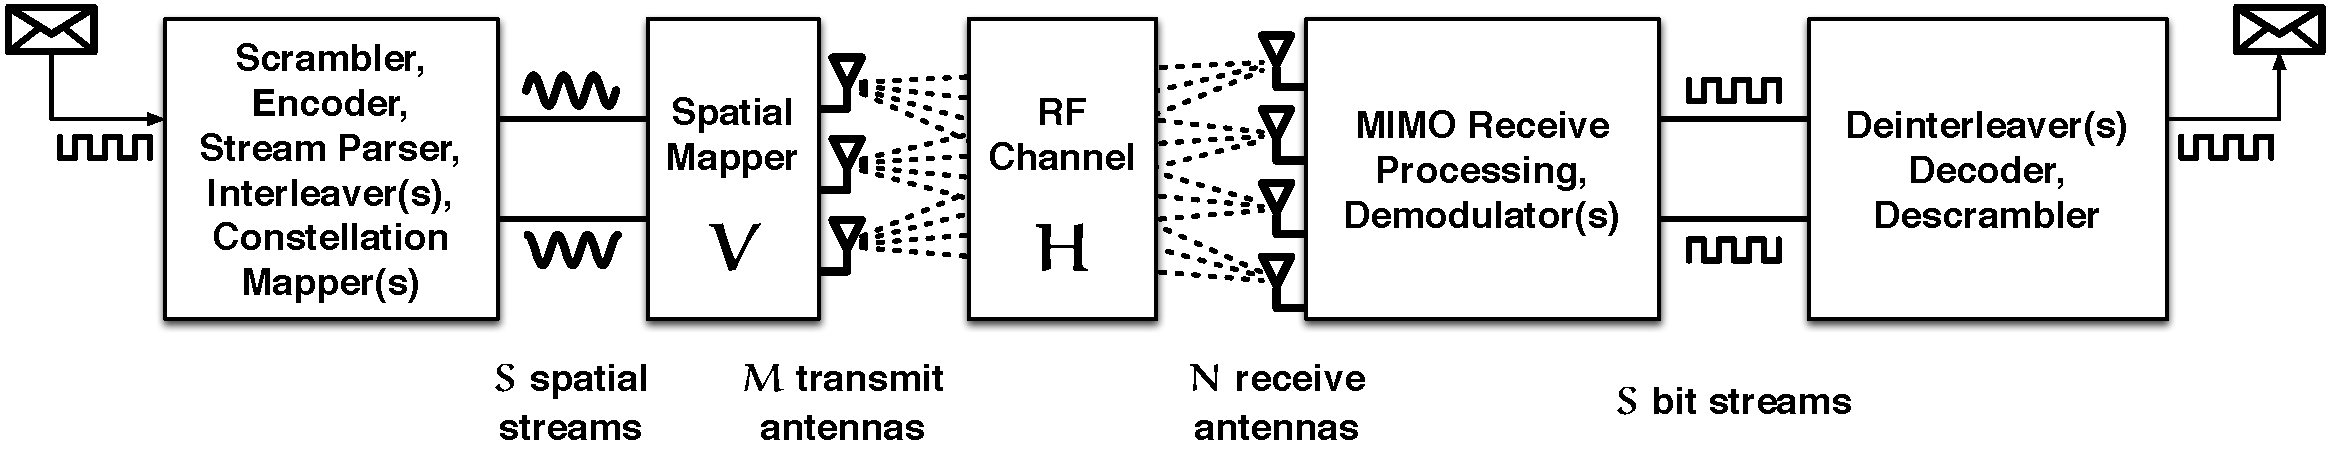
\includegraphics[width=\textwidth]{figures/11n_link_simplified_bigger_fonts.pdf}
\caption[An 802.11n link]{Caption goes here}
\end{figure*}

\begin{figure*}[ht]
\centering
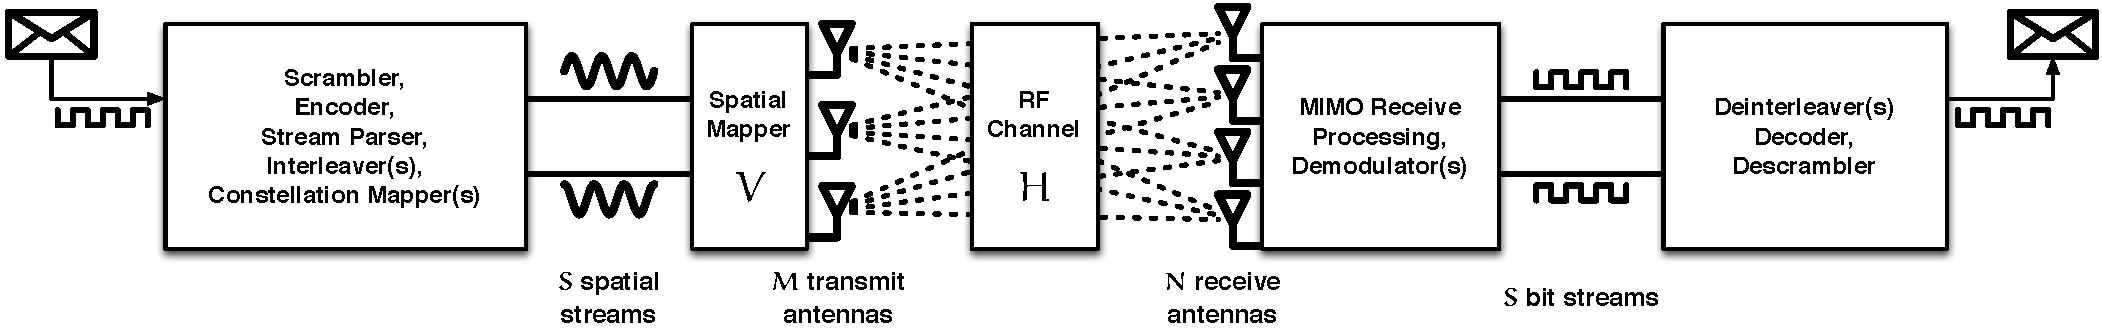
\includegraphics[angle=90,height=\textheight]{figures/11n_link_simplified.pdf}
\caption[An 802.11n link]{Caption goes here}
\end{figure*}

\begin{figure*}[ht!]
\centering
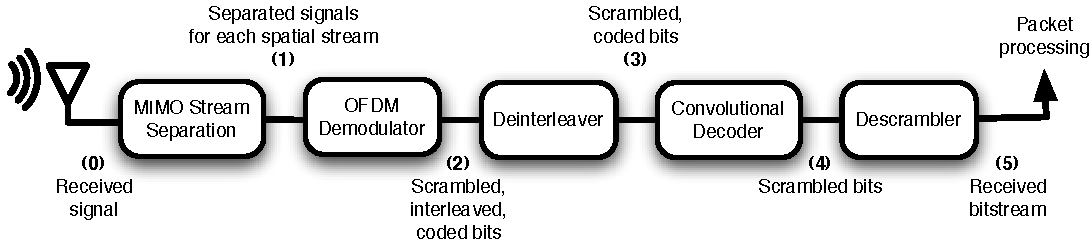
\includegraphics[width=6in]{figures/esnr/mimo_ofdm_decoding_process.pdf}
\caption[The 802.11n MIMO-OFDM decoding process]{\label{fig:ofdm_decoding} The 802.11n MIMO-OFDM decoding process. MIMO receiver separates the RF signal~(0) for each spatial stream~(1). Demodulation converts the separated signals into bits~(2). Bits from the multiple streams are deinterleaved and combined~(3) followed by convolutional decoding~(4) to correct errors. Finally, scrambling that randomizes bit patterns is removed and the packet is processed~(5).}
\end{figure*}

\begin{table}
\centering
%\footnotesize
\begin{tabular}{ccc}
\toprule
Modulation & Bits/Symbol ($k$) & BER$_k$($\rho$) \\
\midrule BPSK & 1 & $Q\left(\sqrt{2\rho}\right)$ \\
QPSK & 2 & $Q\left(\sqrt{\rho}\right)$\\
16-QAM & 4 & $\frac{3}{4}Q\left(\sqrt{\rho/5}\right)$\\
64-QAM & 6 & $\frac{7}{12}Q\left(\sqrt{\rho/21}\right)$\\
\bottomrule
\end{tabular}
\caption[Bit error rate as a function of the symbol SNR for OFDM modulations]{\label{tab:ber_snr}Bit error rate as a function of the symbol SNR $\rho$ for narrowband signals and OFDM modulations. $Q$ is the standard normal CDF\@.}
\end{table}

\heading{Modeling Delivery.}
We build our model up from narrowband demodulation. 
Standard formulas summarized in \tabref{tab:ber_snr} relate SNR (denoted $\rho$) to bit-error rate (BER) for the modulations used in 802.11~\cite{Goldsmith}. CSI gives us the SNR values ($\rho_s$) to use for each subcarrier. For a SISO system, $\rho_s$ is given by the single entry in $H_s$.

In OFDM, decoding is applied across the demodulated bits of subcarriers. If we assume frequency-flat fading for the moment, then all the subcarriers have the same SNR\@. The link will behave the same as in our wired experiments in which RSSI reflect real performance and it will be easy to make predictions for a given SNR and modulation combination. We can use \figref{fig:snr_prr_attenuator} to measure the fixed transition points between rates and thus make our choice.

Frequency-selective fading complicates this picture as some weak subcarriers will be much more likely to have errors than others that are stronger. To model a link in this case, we turn to the notion of an \textbf{\em Effective SNR}\@. This is defined as the SNR that would give the \emph{same error performance on a narrowband channel}~\cite{Nanda_effectiveSNR}. For example, the links in \figref{fig:example_fsf_shape} will have Effective SNR values that are nearly equal because they perform similarly, even though their RSSIs are spread over 15\dB.

The Effective SNR is \emph{not} simply the average subcarrier SNR; indeed, assuming a uniform noise floor, that average is indeed equivalent to the packet SNR derived from the RSSI\@. Instead, the Effective SNR is biased towards the weaker subcarrier SNRs because it is these subcarriers that produce most of the errors. If we ignore coding for the moment, then we can compute the Effective SNR by averaging the subcarrier BERs and then finding the corresponding SNR\@. That is:
\begin{equation}
\label{eq:effective_ber}
	\text{BER}_{\text{eff},k} = \frac{1}{52} \sum \text{BER}_k(\rho_s)
\end{equation}
\begin{equation}
\label{eq:effective_snr}
	\rho_{\text{eff},k} = \text{BER}_k^{-1}(\text{BER}_{\text{eff},k})
\end{equation}
We use $\text{BER}_k^{-1}$ to denote the inverse mapping, from BER to SNR\@. We have also called the average BER across subcarriers the effective BER, $\text{BER}_{\text{eff}}$. SoftRate estimates BER using internal receiver state~\cite{Vutukuru_SoftRate}. We compute it from channel measurements instead.

Note that the BER mapping and hence Effective SNR are functions of the modulation ($k$). That is, unlike the RSSI, a particular wireless channel will have four different Effective SNR values, one describing performance for each of the modulations. In practice, the interesting regions for the four Effective SNRs do not overlap because at a particular Effective SNR value only one modulation will be near the transition from useless (BER $\approx$0.5) to lossless (BER $\approx$0). When graphs in this paper are presented with an Effective SNR axis, we use all four values, each in the appropriate SNR range.

For 802.11n, we also model MIMO processing at the receiver. To do this we need to estimate the subcarrier SNRs for each spatial stream from the channel state matrix $H_s$. Although the standard does not specify receiver processing, 
we assume that a Minimum Mean Square Error (MMSE) receiver is used. It is computationally simple, optimal and equivalent to Maximal-Ratio Combining (MRC) for a single stream, and near optimal for multiple streams. 
All of these make it a likely choice in practice.
%This assumption allows us to use standard formulas to map channel matrices for each subcarrier (from CSI) to per-stream subcarrier SNRs.
%The $N$ per-stream MMSE output SNRs for subcarrier $s$ are 
The SNR of the $i^{\text{th}}$ stream after MMSE processing for subcarrier $s$ is 
given by
\begin{equation}
\centering
\label{eq:mmse_snr}
\rho_{s,i} = \frac{1}{Y_{ii}}-1, \text{ where }
Y = \left(H_s^H H_s+I\right)^{-1}
\end{equation}
for $i \in [1,N]$ and $N$x$N$ identity matrix $I$~\cite{Tse}. For MIMO, the model computes the effective BER averaged across both subcarriers and streams.

Coding interacts with the notion of Effective SNR in a way that is difficult to analyze. One challenge is that the ability to correct bit errors depends on the position of the errors in the data stream. To sidestep this problem, we rely on the interleaving that randomizes the coded bits across subcarriers and spatial streams. Assuming perfect interleaving and robust coding, bit errors in the stream should look no different from bit errors for flat channels (but at a lower SNR). Thus our estimate of the effective BER in \eqref{eq:effective_ber} will accurately reflect the uncoded error performance of the link. Our algorithm now proceeds as in the case of a flat-fading channel described above: we take the computed Effective SNR value and use the measurements from a flat-fading link (\figref{fig:snr_prr_attenuator}) to determine transmission success or failure. As in CHARM~\cite{Judd_CHARM}, we support different packet lengths with different SNR thresholds.

Note that this procedure differs from the typical approach of simulation-based analyses~\cite{Kant_fla, Liu_EESM, Nortel_3g}, that instead map the \emph{uncoded} BER estimate such as we compute to a \emph{coded} BER estimate by means of a simple log-linear approximation. They then use the coded BER estimate, and the length of the target transmission, to directly compute the packet delivery rate of the link. We believe our method of thresholding the Effective SNR is better because it directly accommodates variation in the receiver implementation. Different devices may have different \emph{noise figures}, a measure of how much signal strength is lost in the internal RF circuitry of the NIC\@. They may implement soft Viterbi decoders with more or fewer soft bits for their internal state, or indeed might do hard decoding instead. A receiver could use the optimal Maximum Likelihood MIMO decoder that has exponential complexity for small constellations like BPSK, but revert to the imperfect but more efficient MMSE at higher modulations. All of these can be easily expressed, albeit maybe approximately, as (perhaps modulation-dependent) shifts in the Effective SNR thresholds. In contrast, changing these parameters in the simulation approach involves changing the internals of the calculation.

\heading{Protocol Details.} Effective SNR calculations can be performed by either receiver or transmitter, and each has advantages. For it to make decisions, the transmitter must know the receiver's thresholds for the different rates; these are fixed for a particular model of NIC and can be shared once, e.g., during association. The transmitter also needs up-to-date CSI: either from feedback or estimated from the reverse path. Alternately, the receiver can request rates and select antennas directly using the new Link Adaptation Control field of any 802.11n QoS packet~\cite[\S7.1.3.5a]{80211n}. This obviates sending CSI, but the calculation instead requires that the transmitter share its spatial mappings, i.e.\ how it maps spatial streams to transmit antennas. These are likely to change less frequently than the channel, if at all. Finally, when operating in either mode with fewer transmit streams than antennas, the transmitter must occasionally send a short probe packet with all antennas to measure the full CSI\@.

\heading{Summary and Example.} Combining the above steps, our model consists of the following: 1) CSI is obtained and a test configuration is chosen; 2) the MMSE expression is used to compute per-stream, subcarrier SNRs from the CSI for the test number of streams; 3) the Effective SNR is computed from the per-stream, subcarrier SNRs for the test modulation; and 4) the Effective SNR is compared against the pre-determined threshold for the test modulation and coding to predict whether the link will deliver packets.

\begin{figure}[t]
  \centering
  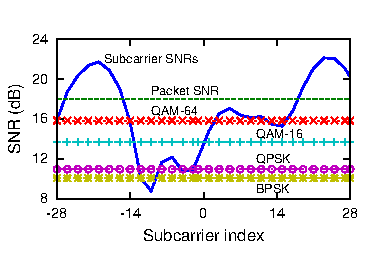
\includegraphics[width=0.9\columnwidth,viewport=0 9 180 111,clip]{figures/esnr/embed_fsf-shape-eff-snr-s3d5-txpower-20.pdf}
  % viewport=0 7 173 113
  \vspace{-4pt}
  \caption{Sample faded link showing the packet SNR and Effective SNRs for different modulations. BPSK has the lowest Effective SNR, but it needs less energy to decode.}
  \label{fig:eff_example}
  \vspace{-3pt}
\end{figure}


As an example, \figref{fig:eff_example} shows the CSI for a SISO link (steps 1--2) as a fading profile across subcarriers, with the computed Effective SNRs for all modulations (step 3). These Effective SNRs are compared with pre-determined thresholds (\figref{fig:snr_prr_attenuator}) to correctly predict that the best working rate will be 39\Mbps. 
Note that these Effective SNRs are well below the RSSI-based packet SNR that is biased towards the stronger subcarriers (note the logarithmic $y$-axis scale). This link does a poor job of harnessing the received power because it is badly faded, so its SNR is a poor predictor of rate.

\begin{table}
\begin{tabular}{ccccccc}
\toprule
\multirow{2}{*}{Algorithm} & \multirow{2}{*}{802.11a/b/g} & \multirow{2}{*}{MIMO} & Antenna & \multirow{2}{*}{TX Power} & Channel & \multirow{2}{*}{Real NICs} \\
& & & Selection & & Width \\
\midrule
SoftRate~\cite{Vutukuru_SoftRate} & \checkmark \\
AccuRate~\cite{Sen_AccuRate} & \checkmark & & & \checkmark & \checkmark \\
EEC~\cite{Chen_EEC} & \checkmark & & & & & \checkmark \\
Effective SNR & \checkmark & \checkmark & \checkmark & \checkmark & \checkmark & \checkmark\\
\bottomrule
\end{tabular}
\caption[Comparison of link error rate prediction algorithms]{\label{tab:algorithm_comparison}A comparison of Effective SNR to other recent algorithms that purport to predict the performance of a wireless link. Effective SNR can predict packet delivery in the largest space because it looks at the raw channel response, whereas the other techniques mostly apply only to single-stream links with fixed antennas and transmit power.}
\end{table}

%%%%%%%%%%%%%%%%%%%%%%%%%%%%%%%%%%
\ifx\mainfile\undefined
%
% ==========   Bibliography   ==========
%
%\nocite{*}   % include everything in the uwthesis.bib file
\bibliographystyle{plain}
\bibliography{dhalperi_thesis}

\end{document}
\fi

\ifx\mainfile\undefined
%  ========================================================================
%  Copyright (c) 2006-2011 The University of Washington
%
%  Licensed under the Apache License, Version 2.0 (the "License");
%  you may not use this file except in compliance with the License.
%  You may obtain a copy of the License at
%
%      http://www.apache.org/licenses/LICENSE-2.0
%
%  Unless required by applicable law or agreed to in writing, software
%  distributed under the License is distributed on an "AS IS" BASIS,
%  WITHOUT WARRANTIES OR CONDITIONS OF ANY KIND, either express or implied.
%  See the License for the specific language governing permissions and
%  limitations under the License.
%  ========================================================================
%
 
\documentclass [11pt, twoside] {uwthesis}

\usepackage{color}
\usepackage{url}
\usepackage{amsmath}
\usepackage{amsfonts}
\usepackage[bookmarks,
	hidelinks,
	plainpages=false,
	pdfpagelabels,
	pagebackref=true,
            ]{hyperref}
\renewcommand*{\backref}[1]{}% for backref < 1.33 necessary
\renewcommand*{\backrefalt}[4]{%
  \ifcase #1 %
    (No citations.)%
  \or
    (Cited on page #2.)%
  \else
    (Cited on pages #2.)%
  \fi
}

\newcommand{\biburl}[1]{{\tt<}\url{#1}{\tt>}}

\hypersetup{%
pdfauthor = {Daniel Chaim Halperin},
pdftitle = {Simplifying the Configuration of 802.11 Wireless Networks with Effective SNR},
pdfsubject = {Ph.D. Dissertation},
pdfkeywords = {},
pdfcreator = {University of Washington, Computer Science and Engineering},
pdfproducer = {},
bookmarksopen = {true},
pdfpagelayout = {TwoColumnRight},
}

\usepackage{footnotebackref}
%%%%%%%%%%%%%%%%%%%%%%%%%%%%%%%%%%%%%%%%%%%%%%%%%%%%%%
%%%        Formatting sections                     %%%
%%%%%%%%%%%%%%%%%%%%%%%%%%%%%%%%%%%%%%%%%%%%%%%%%%%%%%
\newcommand{\algref}[1]{Algorithm~\ref{#1}}
\newcommand{\chapref}[1]{Chapter~\ref{#1}}
\renewcommand{\eqref}[1]{Equation~\ref{#1}}
\newcommand{\figref}[1]{Figure~\ref{#1}}
\newcommand{\secref}[1]{\S\ref{#1}}
\newcommand{\tabref}[1]{Table~\ref{#1}}
\newcommand{\heading}[1]{\vspace{4pt}\noindent\textbf{#1}}
\newcommand{\topheading}[1]{\noindent\textbf{#1}}
\newcommand{\noheading}[0]{\vspace{4pt}\noindent}

%%%%%%%%%%%%%%%%%%%%%%%%%%%%%%%%%%%%%%%%%%%%%%%%%%%%%%
%%%        XXX and other warnings                  %%%
%%%%%%%%%%%%%%%%%%%%%%%%%%%%%%%%%%%%%%%%%%%%%%%%%%%%%%
\newcommand{\xxx}[1]{\textit{\color{red}XXX #1}}

%%%%%%%%%%%%%%%%%%%%%%%%%%%%%%%%%%%%%%%%%%%%%%%%%%%%%%
%%%        Units                                   %%%
%%%%%%%%%%%%%%%%%%%%%%%%%%%%%%%%%%%%%%%%%%%%%%%%%%%%%%
\usepackage{xspace}
\newcommand{\unitsep}{\texorpdfstring{\,}{ }}
\def\unit#1{% from: http://www.tex.ac.uk/cgi-bin/texfaq2html?label=csname "Defining a macro from an argument"
  \expandafter\def\csname #1\endcsname{\unitsep\text{#1}\xspace}%
}
\def\varunit#1#2{% from: http://www.tex.ac.uk/cgi-bin/texfaq2html?label=csname "Defining a macro from an argument"
  \expandafter\def\csname #1\endcsname{\unitsep\text{#2}\xspace}%
}
\unit{GHz}
\unit{MHz}
\unit{kHz}
\unit{Gbps}
\unit{Mbps}
\unit{KB}
\unit{dB}
\unit{dBi}
\unit{dBm}
\unit{W}
\unit{mW}
\varunit{uW}{$\mu$W}
\unit{ms}
\varunit{us}{$\mu$s}
\unit{h}
\unit{m}
\unit{s}
\unit{km}
\unit{cm}
\unit{mm}
\varunit{mmsq}{mm$^\text{2}$}
\varunit{insq}{in$^\text{2}$}
\newcommand{\degree}{\ensuremath{^\circ}\xspace}
\newcommand{\degrees}{\degree}
%%%%%%%%%%%%%%%%%%%%%%%%%%%%%%%%%%%%%%%%%%%%%%%%%%%%%%%%%%%%%%%%%%%%%%%%%%%%%%%%%%%%%%
% Euler for math | Palatino for rm | Helvetica for ss | Courier for tt
%
% From: http://www.tug.org/mactex/fonts/LaTeX_Preamble-Font_Choices.html
%%%%%%%%%%%%%%%%%%%%%%%%%%%%%%%%%%%%%%%%%%%%%%%%%%%%%%%%%%%%%%%%%%%%%%%%%%%%%%%%%%%%%%
\renewcommand{\rmdefault}{ppl} % rm
\usepackage[scaled]{helvet} % ss
\usepackage{courier} % tt
\usepackage{eulervm} % a better implementation of the euler package (not in gwTeX)
\normalfont
\usepackage[T1]{fontenc}
%%%%%%%%%%%%%%%%%%%%%%%%%%%%%%%%%%%%%%%%%%%%%%%%%%%%%%%%%%%%%%%%%%%%%%%%%%%%%%%%%%%%%%

%%%%%%%%%%%%%%%%%%%%%%%%%%%%%%%%%%%%%%%%%%%%%%%%%%%%%%
%%%        Figures                                 %%%
%%%%%%%%%%%%%%%%%%%%%%%%%%%%%%%%%%%%%%%%%%%%%%%%%%%%%%
\usepackage{graphicx}
% Caption package both lets you set the spacing between figure and caption
% and also makes the \figref{} point to the right place.
\usepackage[font=bf,aboveskip=6pt,belowskip=-4mm]{caption}
% Allow subfigures, make them bold
\usepackage[bf,BF,small]{subfigure}
% List of figures
\setcounter{lofdepth}{2}  % Print the chapter and sections to the lot

%%%%%%%%%%%%%%%%%%%%%%%%%%%%%%%%%%%%%%%%%%%%%%%%%%%%%%
%%%        Lists with reduced spacing              %%%
%%%%%%%%%%%%%%%%%%%%%%%%%%%%%%%%%%%%%%%%%%%%%%%%%%%%%%
\usepackage{enumitem}

%%%%%%%%%%%%%%%%%%%%%%%%%%%%%%%%%%%%%%%%%%%%%%%%%%%%%%
%%%        Fancy tables                            %%%
%%%%%%%%%%%%%%%%%%%%%%%%%%%%%%%%%%%%%%%%%%%%%%%%%%%%%%
\usepackage{tabulary}
\usepackage{booktabs}

%%%%%%%%%%%%%%%%%%%%%%%%%%%%%%%%%%%%%%%%%%%%%%%%%%%%%%
%%%        Formatting techniques/tools/etc.        %%%
%%%%%%%%%%%%%%%%%%%%%%%%%%%%%%%%%%%%%%%%%%%%%%%%%%%%%%
\newcommand{\term}[1]{\texttt{#1}}

\begin{document}
 
\textpages
\setcounter{chapter}{4} % Set to n-1!
\fi
%%%%%%%%%%%%%%%%%%%%%%%%%%%%%%%%%%

\cleardoublepage
\chapter{Measuring 802.11\texorpdfstring{\lowercase{n}}{n} Traces with Channel State Information}
\label{chap:tool}

In this section, we describe our preliminary work building an experimental 802.11n platform, in particular a tool that uses commodity Intel Wi-FI NICs to measure the 802.11n Channel State Information. Next, we use measurements of packet delivery vs RSSI and CSI to show explain why RSSI fails to predict packet delivery in real wireless channels. When then use CSI in conjunction with the concept of an Effective SNR for wireless links to explain the performance of links that experience frequency-selective fading. We demonstrate experimentally that CSI and Effective SNR can predict the performance of wireless links across a wide range of configurations, such as rate selection and transmit power control. Finally, we present trace-driven simulation results that show that a simple Effective SNR-based rate \emph{selection} (not \emph{adaptation}) can be used to achieve good performance in varying channels.

\section{802.11n CSI Tool and Experimental Platform}
\label{sec:platform}
In conjunction with Intel Labs Seattle, we have built an experimental 802.11n platform that uses the Intel Wi-Fi Wireless Link 5300 (\program{iwl5300}) 802.11a/b/g/n network cards. We modified the closed-source firmware and open-source Linux driver to add a number of experimental features importantly to measure the 802.11n CSI\@. Here, we summarize these features.

\heading{802.11n CSI Measurement.} The channel sounding mechanism added in 802.11n defines a management frame used to report the CSI from the receiver of a frame back to the transmitter. This mechanism is intended for calibration or to inform transmit beamforming, and we co-opt it for our experiments. We configure the NIC with a debug mode to compute this feedback packet for every received frame,\footnote{CSI is reported for correctly received frames destined for the measurement node or sent to a special hard-coded broadcast address.} rather than just during sounding, and send it up to the driver instead of back to the transmitter. The \program{iwl5300} provides CSI in a format that reports the channel matrices for 30 subcarrier groups, which is about one group for every 2 subcarriers at 20\MHz or every 4 subcarriers at 40\MHz. Each channel matrix entry is a complex number, with signed 8-bit resolution each for the real and imaginary parts. It specifies the gain and phase of the spatial path between a single transmit-receive antenna pair. Intel's implementation of the 802.11n CSI does not include per-subcarrier noise measurements, so we assume the noise floor is uniform across all subcarriers to compute SNRs. This is consistent with white noise observed on other OFDM platforms~\cite{Rahul_FARA}.

\heading{RSSI Measurement.} 
For each received packet the NIC reports the traditional metrics of RSSI per receive antenna, noise floor and the setting on the automatic gain controlled (AGC) amplifier. These combine to define the per-receive-chain packet SNR ($\rho_{\text{packet}}$):
\begin{equation}
\label{eq:per_chain_snr}
	\rho_{\text{packet}} = \text{RSSI (dBm)} - \text{Noise (dBm)} - \text{AGC (dB)}
\end{equation}
The \program{iwl5300} calculates the quantities RSSI and Noise as the respective sums of average signal strength and average error vector magnitude in each OFDM subcarrier~\cite{iwlwifi}. This is exactly the traditional definition of SNR applied to OFDM\@.

\heading{Transmit Power Control.} Our hardware enables us to vary the transmit power level from $-$10\dBm~(100\uW) to $+$16\dBm~(40\mW) in steps of 0.5\dB, and divides power equally across streams. Additionally, the \program{iwl5300} reduces the transmit power slightly when using the highest single-stream rates to avoid distortions caused by passing 64-QAM symbols with high peak-to-average power ratio through the transmit amplifier.

\heading{Rapid Rate Variation.} In normal operation, the \program{iwl5300} decouples queuing packets for transmission from selecting rates for these packets, since queues must be kept large to take advantage of 802.11n block transmissions. This makes it difficult to control the rate at which individual packets are transmitted. We modified the firmware and driver to support the transmission of individual packets at predetermined rates, and added driver-level code to rapidly iterate through a user-configurable set of available rates.

\heading{Userspace Connector.} We used the Linux kernel \program{connector} framework to implement a low-latency socket-based communication channel between the kernel driver and userspace utilities. This enables userspace utilities to log CSI and other output from the driver, and send messages that, e.g., change the currently selected rate or antennas or change the transmit power level.

\heading{Publicly Released Tool.} We have publicly released our experimental platform and CSI collection tool in the form of open source drivers, userspace utilities, MATLAB code, and binary firmware image~\cite{Halperin_csitool}. At the time of writing, we are aware of several users, including multiple research and product groups within Intel, industrial researchers at HP Labs, and academic researchers at UT Austin, CMU, UCL, and the Hong Kong University of Science and Technology.

\heading{Papers based on it.} PinLoc~\cite{Sen_PinLoc}, SpinLoc~\cite{Sen_SpinLoc}, CSI-SF~\cite{Crepaldi_CSI_SF}, Frequency Diversity~\cite{Bhartia_FreqDiv}. Doppler~\cite{Perahia_Doppler}.

%%%%%%%%%%%%%%%%%%%%%%%%%%%%%%%%%%
\ifx\mainfile\undefined
%
% ==========   Bibliography   ==========
%
%\nocite{*}   % include everything in the uwthesis.bib file
\bibliographystyle{plain}
\bibliography{dhalperi_thesis}

\end{document}
\fi
\ifx\mainfile\undefined
%  ========================================================================
%  Copyright (c) 2006-2011 The University of Washington
%
%  Licensed under the Apache License, Version 2.0 (the "License");
%  you may not use this file except in compliance with the License.
%  You may obtain a copy of the License at
%
%      http://www.apache.org/licenses/LICENSE-2.0
%
%  Unless required by applicable law or agreed to in writing, software
%  distributed under the License is distributed on an "AS IS" BASIS,
%  WITHOUT WARRANTIES OR CONDITIONS OF ANY KIND, either express or implied.
%  See the License for the specific language governing permissions and
%  limitations under the License.
%  ========================================================================
%
 
\documentclass [11pt, twoside] {uwthesis}

\usepackage{color}
\usepackage{url}
\usepackage{amsmath}
\usepackage{amsfonts}
\usepackage[bookmarks,
	hidelinks,
	plainpages=false,
	pdfpagelabels,
	pagebackref=true,
            ]{hyperref}
\renewcommand*{\backref}[1]{}% for backref < 1.33 necessary
\renewcommand*{\backrefalt}[4]{%
  \ifcase #1 %
    (No citations.)%
  \or
    (Cited on page #2.)%
  \else
    (Cited on pages #2.)%
  \fi
}

\newcommand{\biburl}[1]{{\tt<}\url{#1}{\tt>}}

\hypersetup{%
pdfauthor = {Daniel Chaim Halperin},
pdftitle = {Simplifying the Configuration of 802.11 Wireless Networks with Effective SNR},
pdfsubject = {Ph.D. Dissertation},
pdfkeywords = {},
pdfcreator = {University of Washington, Computer Science and Engineering},
pdfproducer = {},
bookmarksopen = {true},
pdfpagelayout = {TwoColumnRight},
}

\usepackage{footnotebackref}
%%%%%%%%%%%%%%%%%%%%%%%%%%%%%%%%%%%%%%%%%%%%%%%%%%%%%%
%%%        Formatting sections                     %%%
%%%%%%%%%%%%%%%%%%%%%%%%%%%%%%%%%%%%%%%%%%%%%%%%%%%%%%
\newcommand{\algref}[1]{Algorithm~\ref{#1}}
\newcommand{\chapref}[1]{Chapter~\ref{#1}}
\renewcommand{\eqref}[1]{Equation~\ref{#1}}
\newcommand{\figref}[1]{Figure~\ref{#1}}
\newcommand{\secref}[1]{\S\ref{#1}}
\newcommand{\tabref}[1]{Table~\ref{#1}}
\newcommand{\heading}[1]{\vspace{4pt}\noindent\textbf{#1}}
\newcommand{\topheading}[1]{\noindent\textbf{#1}}
\newcommand{\noheading}[0]{\vspace{4pt}\noindent}

%%%%%%%%%%%%%%%%%%%%%%%%%%%%%%%%%%%%%%%%%%%%%%%%%%%%%%
%%%        XXX and other warnings                  %%%
%%%%%%%%%%%%%%%%%%%%%%%%%%%%%%%%%%%%%%%%%%%%%%%%%%%%%%
\newcommand{\xxx}[1]{\textit{\color{red}XXX #1}}

%%%%%%%%%%%%%%%%%%%%%%%%%%%%%%%%%%%%%%%%%%%%%%%%%%%%%%
%%%        Units                                   %%%
%%%%%%%%%%%%%%%%%%%%%%%%%%%%%%%%%%%%%%%%%%%%%%%%%%%%%%
\usepackage{xspace}
\newcommand{\unitsep}{\texorpdfstring{\,}{ }}
\def\unit#1{% from: http://www.tex.ac.uk/cgi-bin/texfaq2html?label=csname "Defining a macro from an argument"
  \expandafter\def\csname #1\endcsname{\unitsep\text{#1}\xspace}%
}
\def\varunit#1#2{% from: http://www.tex.ac.uk/cgi-bin/texfaq2html?label=csname "Defining a macro from an argument"
  \expandafter\def\csname #1\endcsname{\unitsep\text{#2}\xspace}%
}
\unit{GHz}
\unit{MHz}
\unit{kHz}
\unit{Gbps}
\unit{Mbps}
\unit{KB}
\unit{dB}
\unit{dBi}
\unit{dBm}
\unit{W}
\unit{mW}
\varunit{uW}{$\mu$W}
\unit{ms}
\varunit{us}{$\mu$s}
\unit{h}
\unit{m}
\unit{s}
\unit{km}
\unit{cm}
\unit{mm}
\varunit{mmsq}{mm$^\text{2}$}
\varunit{insq}{in$^\text{2}$}
\newcommand{\degree}{\ensuremath{^\circ}\xspace}
\newcommand{\degrees}{\degree}
%%%%%%%%%%%%%%%%%%%%%%%%%%%%%%%%%%%%%%%%%%%%%%%%%%%%%%%%%%%%%%%%%%%%%%%%%%%%%%%%%%%%%%
% Euler for math | Palatino for rm | Helvetica for ss | Courier for tt
%
% From: http://www.tug.org/mactex/fonts/LaTeX_Preamble-Font_Choices.html
%%%%%%%%%%%%%%%%%%%%%%%%%%%%%%%%%%%%%%%%%%%%%%%%%%%%%%%%%%%%%%%%%%%%%%%%%%%%%%%%%%%%%%
\renewcommand{\rmdefault}{ppl} % rm
\usepackage[scaled]{helvet} % ss
\usepackage{courier} % tt
\usepackage{eulervm} % a better implementation of the euler package (not in gwTeX)
\normalfont
\usepackage[T1]{fontenc}
%%%%%%%%%%%%%%%%%%%%%%%%%%%%%%%%%%%%%%%%%%%%%%%%%%%%%%%%%%%%%%%%%%%%%%%%%%%%%%%%%%%%%%

%%%%%%%%%%%%%%%%%%%%%%%%%%%%%%%%%%%%%%%%%%%%%%%%%%%%%%
%%%        Figures                                 %%%
%%%%%%%%%%%%%%%%%%%%%%%%%%%%%%%%%%%%%%%%%%%%%%%%%%%%%%
\usepackage{graphicx}
% Caption package both lets you set the spacing between figure and caption
% and also makes the \figref{} point to the right place.
\usepackage[font=bf,aboveskip=6pt,belowskip=-4mm]{caption}
% Allow subfigures, make them bold
\usepackage[bf,BF,small]{subfigure}
% List of figures
\setcounter{lofdepth}{2}  % Print the chapter and sections to the lot

%%%%%%%%%%%%%%%%%%%%%%%%%%%%%%%%%%%%%%%%%%%%%%%%%%%%%%
%%%        Lists with reduced spacing              %%%
%%%%%%%%%%%%%%%%%%%%%%%%%%%%%%%%%%%%%%%%%%%%%%%%%%%%%%
\usepackage{enumitem}

%%%%%%%%%%%%%%%%%%%%%%%%%%%%%%%%%%%%%%%%%%%%%%%%%%%%%%
%%%        Fancy tables                            %%%
%%%%%%%%%%%%%%%%%%%%%%%%%%%%%%%%%%%%%%%%%%%%%%%%%%%%%%
\usepackage{tabulary}
\usepackage{booktabs}

%%%%%%%%%%%%%%%%%%%%%%%%%%%%%%%%%%%%%%%%%%%%%%%%%%%%%%
%%%        Formatting techniques/tools/etc.        %%%
%%%%%%%%%%%%%%%%%%%%%%%%%%%%%%%%%%%%%%%%%%%%%%%%%%%%%%
\newcommand{\term}[1]{\texttt{#1}}

\begin{document}
 
\textpages
\setcounter{chapter}{5} % Set to n-1!
\fi
%%%%%%%%%%%%%%%%%%%%%%%%%%%%%%%%%%

\cleardoublepage
\chapter{Packet Delivery over MIMO Channels}
\label{chap:delivery}

In this chapter, I experimentally evaluate how well my Effective SNR model predicts packet delivery for 802.11n wireless links. This is the fundamental measure of whether the model can be useful; good predictions are necessary to properly configure links and networks to solve the link and network configuration problems.

To do so, I use my CSI measurement tool to gather a wide range of channel and performance information across 200 wireless links in both testbeds. This captures a wide variety of fading environments, from line-of-sight links in the same room to links between nodes in different rooms with RF barriers and reflectors spread around and between them. I then use this data to evaluate the accuracy of predictions made when using Packet SNR and Effective SNR.

The primary study in this chapter determines how accurately Packet SNR and Effective SNR predict whether packets will be delivered using different modulation and coding schemes. I then consider how well CSI measurements enable predictions about the effects of transmit power control to show its flexibility. I conclude this chapter by evaluating the resilience of my Effective SNR system to interference. These three studies lay the foundation for showing that Effective SNR is accurate, flexible, and practical; in subsequent chapters I deploy my model as part of a system in the context of many application-related configuration problems.

\section{Experimental Data}
I measured packet delivery over a 20\MHz channel on my two 802.11n testbeds, using links with four different antenna configurations:
\begin{enumerate}
\item The \textbf{SISO} configuration uses a single antenna at each node. This configuration corresponds to 802.11a.
\item The \textbf{SIMO} configuration uses a single transmit antenna but three receive antennas. This is an 802.11a/g/n configuration that uses spatial diversity techniques.
\item The \textbf{MIMO2} configuration uses two spatial streams and three receive antennas. This employs both 802.11n techniques of spatial multiplexing and spatial diversity.
\item The \textbf{MIMO3} configuration uses three antennas at each node to send and receive three spatial streams. This configuration uses spatial multiplexing, but does not additionally benefit from spatial diversity.
\end{enumerate}

For each of these configurations, I measured the packet delivery for each link using each MCS, at at each transmit power level between $-$10\dBm and $+$16\dBm in steps of 2\dB. I sent 1,500-byte packets as constant bit-rate UDP traffic generated by \program{iperf} at 2\Mbps for 5 seconds, about 860 packets total. The receiver also recorded the CSI and per antenna RSSIs and noise floors to measure the RF channel for each correctly received packet. In these experiments, I turned off 802.11's link layer retransmissions in order to observe the underlying packet delivery rate. The experiments were conducted at night on unused 802.11 channels in order to minimize the effects of environmental movement and RF interference on these results.

%Note that CSI and RSSI are measured during the preamble, and so do not depend on the transmit rate, though they vary with the number of streams. 
%Similarly, 3x3 CSI gives us the channel between each pair of transmit and receive antennas, so it also implicitly contains 1x1 CSI\@.

The above testing gives ground truth data to probe variation across 200 links, 26\dB of transmit power, four antenna configurations ranging from SISO to MIMO3, and 8 MCS values per configuration. This covers all of the key variables needed to implement and evaluate my Effective SNR model. 

\section{Results}
The goal of this chapter is to understand whether Effective SNR is a good metric, whether it is an accurate predictor of packet delivery. In this section, I evaluate this in two ways. The first is via the \define{transition window}, i.e., the SNR regime in which packet delivery for all links goes from near-zero to near-perfect. We saw in \chapref{chap:problem} that this transition occurs rapidly for a wired link (\figref{fig:snr_prr_attenuator}), but occurs over a wide range for wireless links (\figref{fig:snr_prr_26_65}) when using the Packet SNR. A narrow transition window would be one indicator that Effective SNR works well.

The second evaluation metric is \define{rate confusion}, i.e., how many rates might be best at a particular SNR value. The wired link showed clear separation between rates, such that at every SNR value there is a clear best rate. Conversely, because the transition regions of different wireless links overlap, links with the same Packet SNR might support very different rates. Here, I compare the degree of rate confusion between Packet SNR Effective SNR.

\subsection{Transition Windows}
\begin{table}
\centering
\begin{tabular}{cccccc}
\toprule
\multirow{2}{*}{MCS} & \multirow{2}{*}{Rate (Mbps)} & \multicolumn{2}{c}{$\Delta\rho_{\text{packet}}$ (dB)} &
\multicolumn{2}{c}{$\Delta\rho_{\text{eff}}$ (dB)} \\ 
\cmidrule(lr){3-4} \cmidrule(lr){5-6}
& &  ~~5\%--95\% & ~25\%--75\% & ~~5\%--95\% & ~25\%--75\%  \\
\midrule 
0 &  6.5                    & 3.08  & 1.29  & 2.05  & 0.81 \\
1 & 13.0                    & 3.45  & 1.44  & 2.38  & 0.89 \\
2 & 19.5                    & 6.27  & 3.12  & 2.30  & 0.85 \\
3 & 26.0                    & 3.93  & 1.98  & 3.02  & 0.94 \\
4 & 39.0                    & 7.05  & 3.49  & 2.19  & 0.93 \\
5 & 52.0                    & 7.16  & 3.20  & 2.29  & 1.06 \\
6 & 58.5                    & 7.25  & 3.37  & 2.92  & 1.41 \\
7 & 65.0                    & 7.24  & 2.81  & 2.92  & 1.35 \\
\midrule
\multicolumn{2}{c}{Average} & 5.68  & 2.59  & 2.51  & 1.03 \\         
\bottomrule
\end{tabular}
\caption[Width of SISO transition windows]{\label{tab:transitions} Width of SISO transition windows.}
\end{table}

I analyzed the SISO measurements to find the transition window for each of the measured links. I define the window to be the SNR values between which packet delivery rises from 10\% (lossy) to 90\% (reliable) for any link.

\tabref{tab:transitions} gives the width of the transition window (denoted $\Delta\rho$) for SISO rates using the Packet SNR and Effective SNR metrics. I show the 25\%--75\% range of points in the transition window as a measure of the typical link, and the 5\%--95\% range as a measure of most links. A good result here is a narrow window like that measured over a wire (\figref{fig:snr_prr_attenuator}).

The table shows that the transition widths are consistently tight with my model. Most links transition within a window of around 2\dB for most rates. The width of the SNR-based transition windows is typically two to three times looser, especially for the denser modulation schemes like 64-QAM and higher code rates. This means that it is easy for a less than ideal channel to degrade the reception of high rates. However, while the transitions for the last four rates are inflated with SNR, they remain tight with Effective SNR\@. 

The results for Effective SNR are in fact about the best that can be obtained because they are close to textbook transitions for flat-fading channels and those measured over a wire (\figref{fig:snr_prr_attenuator}). A small improvement is surely possible, but this is probably limited by the precision of my measurement data. The IWL5300 gives RSSI, AGC and noise values in dB to the nearest integer, and at most 8-bit CSI over a 48\dB range for 30 out of 56 subcarriers. With these factors, quantization error of at least 1\dB is likely.

The larger significance of narrow transition windows is that, by reducing them enough that they do not overlap, I can unambiguously predict the highest rate that will work for nearly all links nearly all of the time. In contrast, Packet SNR transition windows overlap such that for a given SNR there may be five different best rates across links the testbed. I explore this in the next section.


\subsection{Rate Confusion}
\label{sec:rate_confusion}

\begin{figure}[p]
	\begin{leftfullpage}
	\centering
	\subfigure[SISO configurations]{
		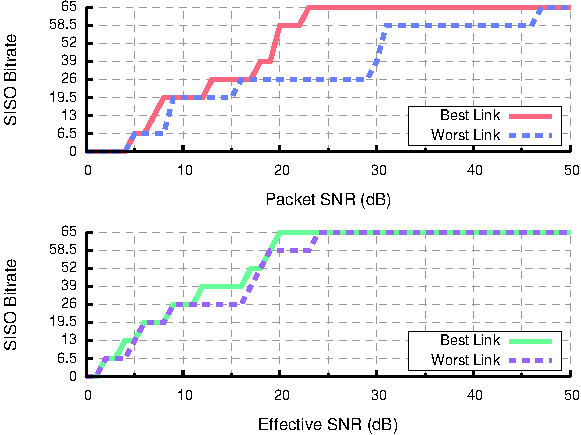
\includegraphics[width=0.8\textwidth]{figures/delivery_figures/siso_rate_confusion.pdf}%
		\label{fig:snr_rate_step_1x1}%
	}%
	
	\subfigure[SIMO configurations]{
		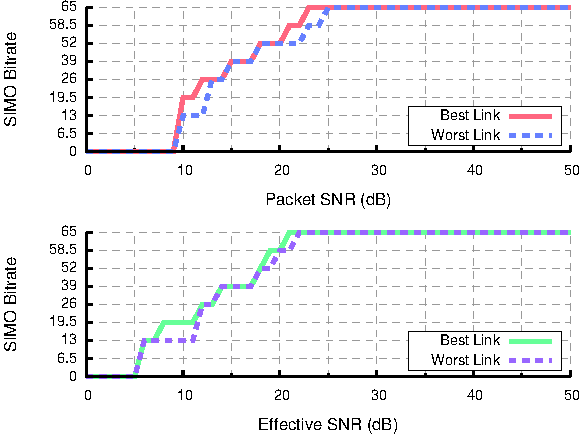
\includegraphics[width=0.8\textwidth]{figures/delivery_figures/simo_rate_confusion.pdf}%
		\label{fig:snr_rate_step_1x3}%
	}
	\caption[Rate confusion with Packet SNR and Effective SNR for different antenna configurations]{\label{fig:snr_rate_steps}Rate confusion with Packet SNR and Effective SNR. Excepting very low and high SNRs, one Packet SNR value maps to multiple best rates for different links. For the same data, 
Effective SNR provides a clear indicator of the best rate for nearly all links.}
	\end{leftfullpage}
\end{figure}

\setcounter{figure}{0}
\begin{figure}
\begin{xtrafullpage}
	\centering	
	\setcounter{subfigure}{2}
	\subfigure[MIMO2 configurations]{
		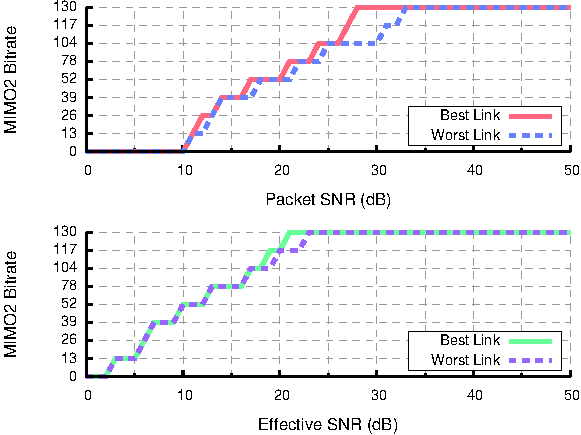
\includegraphics[width=0.8\textwidth]{figures/delivery_figures/mimo2_rate_confusion.pdf}%
		\label{fig:snr_rate_step_2x3}%
	}%

	\subfigure[MIMO3 configurations]{
		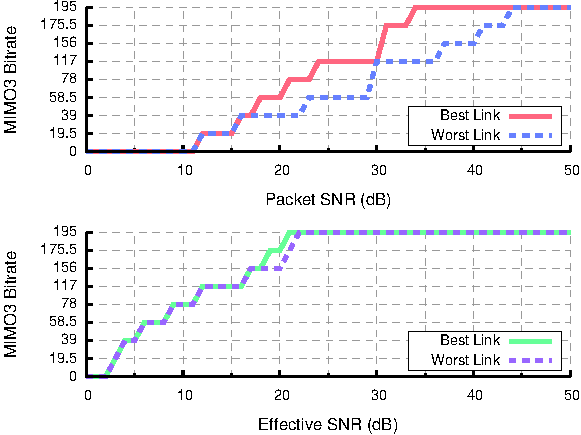
\includegraphics[width=0.8\textwidth]{figures/delivery_figures/mimo3_rate_confusion.pdf}%
		\label{fig:snr_rate_step_3x3}%
	}
	\vspace{36pt}
\end{xtrafullpage}
\end{figure}

To understand whether the Effective SNR model accurately predicts packet delivery, I analyze the fastest working rate (PRR$\geq$ 90\%) for each link and all NIC settings. \figref{fig:snr_rate_steps} shows the results broken down by configuration. The SISO experiment (\figref{fig:snr_rate_step_1x1}) shows links for both testbeds combined. The remaining graphs \figref{fig:snr_rate_step_1x3}--\ref{fig:snr_rate_step_3x3}  show rates for SIMO, MIMO2 and MIMO3 configurations for the Intel testbed only; it is denser than UW and supports MIMO experiments over our NIC's transmit power range.

These graphs study rate confusion, i.e., the ability of a given SNR value to predict the best rate across a wide set of links. If we consider the fastest rate each link supports at a particular Packet SNR or Effective SNR value, the best link is the link that supports the fastest rate, and the worst link is the slowest. The difference between the best and worst links, i.e., the set of possible best rates for an arbitrary link with a particular SNR, is the rate confusion. I plot this spread in these graphs. Note that the SIMO figure does not include data for the lowest 6.5\Mbps rate, because very few links experience loss at that rate within the transmit power range of the IWL5300---the added spatial diversity makes most links work well, as described below.

Ideally, the best and worst lines would overlap completely, such that the highest rate for a given SNR would be the same for the best and worst links. This rate would then be an accurate prediction for the particular Effective SNR or Packet SNR level. Conversely, gaps between the best and worst lines expose confusion about which rate will be the highest rate for that SNR.

For the SISO (\figref{fig:snr_rate_step_1x1}) and MIMO3 (\figref{fig:snr_rate_step_3x3}) cases, the figures show that using Packet SNR results in a large spread between the best and worst lines. Except for extremely low and high SNRs, nearly all SNRs have at least two---and up to five different---rates as suitable choices for the best rate. That is, Packet SNR often poorly indicates rate.

In sharp contrast, %looking at bottom lines in the graphs, 
the two Effective SNR lines overlap almost all the time, and mostly appear to be a single line. This is almost an ideal result. Effective SNR is a clear indicator of best rate. When there is slight separation, the spread is only between rates that use the same modulation but different amounts of coding. These combinations are also close together in our wired experiments. 

Interestingly, these results show that Packet SNR predictions are much better for the SIMO and MIMO3 cases, though still not as accurate as Effective SNR, particularly for the highest rates. The reason is \emph{spatial diversity}: spare receive antennas gather the received signal and combine to make the channel more frequency-flat, thus bringing the Packet SNR closer to the Effective SNR. This effect is well-known, though typically not observable using real 802.11 NICs which, except my prototype implementation, do not export CSI. This result suggests that Packet SNR \emph{is} a reasonable predictor for an 802.11 configuration with significant diversity. Still, observe that Packet SNR does not transfer well across the antenna modes (as diversity gains and inter-stream interference change unpredictably) which makes this less useful. This is one reason that SISO rate adaptation schemes do not translate to MIMO.

Finally, I note that neither Effective SNR nor Packet SNR performs extremely well at the lowest modulation at low SNRs. I believe this artifact arises from errors in the AGC values reported by the NIC, observed by Judd et al.~\cite{Judd_CHARM} and confirmed by my data for Intel's hardware.

\section{Transmit Power Control}
\label{sec:tx_power_trim}
The results so far show we can predict delivery over a range of transmit powers (as well as other choices). I now show that CSI measured at one transmit power level is useful to predict delivery at a different power level. This is valuable for power control applications, e.g., pruning excess power to reduce co-channel interference~\cite{Monks_PowerMAC,Ramachandran_Symphony,Son_PowerStudy}. 

\begin{figure}[t]
  \centering
  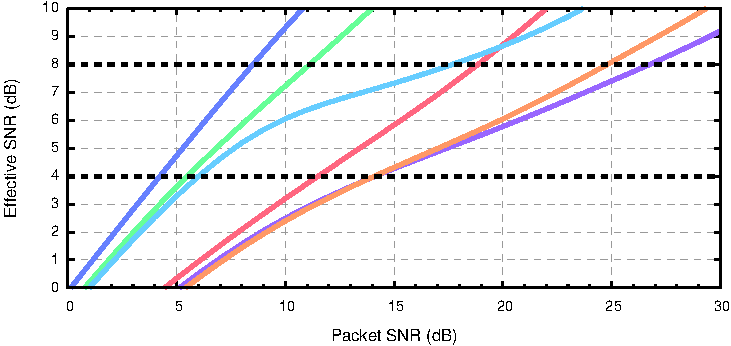
\includegraphics[width=\textwidth]{figures/eff_vs_snr_qpsk.pdf}
  \caption[Effective SNR vs Packet SNR for four faded links]{Effective SNR (for QPSK) versus Packet SNR for flat (left) to faded (right) links.}
  \label{fig:eff_vs_rssi}
\end{figure}

Note that changing transmit power has a different effect (in terms of delivery and highest rate) on real links even if they start at exactly the same rate and SNR. \figref{fig:eff_vs_rssi} plots the Packet SNR versus Effective SNR relationship for six example 1x1 links in T1 and T2.
I compute this data by scaling the CSI measured at maximum transmit power over a range of power levels.
The links range from near-flat to deeply-faded. Correspondingly, they have different slopes. On the left, Packet SNR matches Effective SNR for the nearly flat link. 
However, for the right-most, deeply faded links, the Packet SNR decreases from 25\dB to 15\dB (10$\times$ transmit power reduction) as the Effective SNR only drops by 4\dB (2.5$\times$). This difference in how links harness power makes transmit power control non-trivial.


\begin{figure}[t]
      \centering
      \subfigure[Predicted and measured power saving]{%
      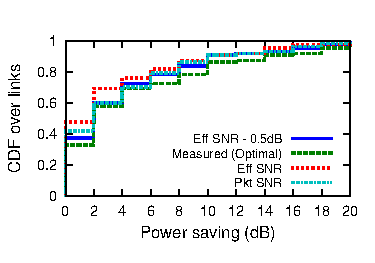
\includegraphics[width=0.5\columnwidth,viewport=0 7 195 110,clip]{figures/power_save_1x1.pdf}%
      \label{fig:power_save_cdf}%
      }%
      \subfigure[Measured PRR corresponding to reduced TX power levels]{%
      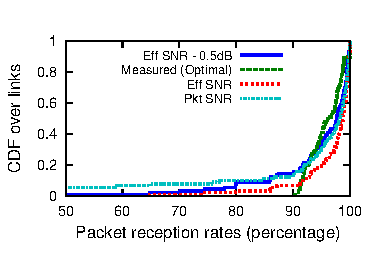
\includegraphics[width=0.5\columnwidth,viewport=0 7 195 110,clip]{figures/power_save_final_prr_1x1.pdf}%
      \label{fig:power_prr_cdf}%
      }%
      \caption[Impact of pruning excess transmit power]{\label{fig:power_save_1x1} Power saving and performance impact of pruning excess transmit power. Pruning with Effective SNR is tight (within 0.5\dB) and does not degrade performance. Pruning with packet SNR degrades performance more without much extra savings.} 
\end{figure}

To test predictions across power levels, I consider the goal of trimming excess transmit power, i.e. power that can be removed without causing the highest rate for the link to drop. These experiments start with 88 SISO links from the Intel Labs Testbed configured to radiate 10\mW of transmit power, and one CSI sample per link. Considering transmit power reductions in increments of 2\dB, the Effective SNR model can predict the best supported rate for each reduced power level, and choose the lower power level with the same best rate. The measurements described earlier include the ground truth packet reception ratio for each power level, and thus these data can be used to check the accuracy of the predictions.

\figref{fig:power_save_1x1} shows the power savings and performance degradation of four different threshold schemes.
A good result here is power savings without a loss of performance; the absolute amount of power savings is not meaningful as it depends on the testbed.
The Measured (Optimal) line shows the best that can be done. Measured PRRs at all power levels are used to guide power control decisions. Therefore, the final delivery probabilities are hardly decreased (all links have PRR$>$90\%), yet most links save a little power and some save a lot. %of power.

The graphs show that using Effective SNR to predict how much power to trim has a similarly good tradeoff. Impact on rate remains limited, yet power is saved, more than 10\dB for around 10\% of the links. The gap between the Measured and the Eff SNR lines is due to the fact the Eff SNR thresholds might be slightly conservative for some links. To show that this trimming is tight, consider trimming towards slightly lower thresholds ($\text{Effective SNR}-\text{0.5\dB}$, solid line). This results in little additional power savings, but degrades more links so that they work partially. In comparison, the Pkt SNR line shows the effects of using Packet SNR to save power. The savings are barely increased, but several links are degraded to the point that some stop working altogether.

\section{Interference}
\label{sec:interference}
Finally, it is important to investigate how an Effective SNR-based protocol can cope with interference. This is one of the largest potential weaknesses of this technique, because Effective SNR is based on measurements taken only during the packet preamble.% There are three important components of dealing with interference: 1) maintaining an accurate estimate of interference-free link quality, so that transient interference doesn't cause wild rate swings; 2) recognizing collisions when they occur, to avoid unnecessary rate fallback; and 3) providing an estimate of link quality that enables efficient operation during persistent interference.

I studied the variation of CSI measurements during interference. I chose two nodes at UW that do not detect each other with carrier sense and sent large packets designed to collide, while monitoring the CSI recorded by all other receiving nodes. I also varied the transmit power of the node designated as the interferer from low to high to induce a large range of interfering channels. For all but one of 20 links, the rate predicted by the majority of CSI measurements for correct packets was the same with and without interference; the remaining link was off by a single rate. From these measurements, we can conclude that the mere presence of interference does not completely invalidate Effective SNR values, and thus transient interference will not cause wild swings in transmit rate.

However, for continuous interference Effective SNR will provide an aggressive estimate, and will need another way to compensate. This should be reflected in larger noise floor measurements by the NIC,\footnote{Note that OFDM does not turn interference into inflated RSSI as do the spread spectrum modulations used in 802.11b.} however the platform does not provide this information for dropped packets. An alternative, that I have not yet explored, might be an \define{Effective SINR} metric that incorporates CSI measurements from the interfering nodes to predict packet delivery.

%Because it does not use packet loss as a signal, ESNR will not conservatively reduce rate during interference. Thus transient interference will only cause transient interruptions. However, the Effective SNR measured in a single packet preamble simply does not provide an estimate of link quality when the link experiences persistent interference. One solution is to leverage SoftRate in these circumstances; while Effective SNR can guide the overall choice of antennas and number of spatial streams, SoftRate's continuous estimate of BER may be better suited for choosing rates within one mode. An alternative (that we have not yet explored) might be an \emph{Effective SINR} metric incorporating CSI measurements from the interfering nodes to predict packet delivery.

To recognize collisions, I propose to leverage a new MAC feature of the 802.11n packet aggregation mechanism. Block ACKs selectively acknowledge frames in a batch of packets transmitted as one continuous burst. Each packet in the burst has a separate checksum, and thus the Block ACK serves as block-based feedback of packet correctness as the block-based checksums analyzed in PPR~\cite{Jamieson_PPR}. We can therefore use the error patterns in the Block ACK to recognize collisions: when the rate is overselected, errors should be randomly distributed throughout the batch, and bursty when a collision clobbers a continuous part of the batch.

\section{Summary}
From these results, I conclude that Effective SNR consistently and accurately indicates the best rate for nearly all links and all configurations without any per-link calibration. The low degree of rate confusion with Effective SNR in \secref{sec:rate_confusion} implies that it should be possible to define SNR thresholds that clearly define when a rate will work well. I discuss how to choose these thresholds in the next chapter,\footnote{\textcolor{red}{XXX: or, where should this be? It's not really necessary yet, not until we start making algorithmic choices.}}. The results in \secref{sec:tx_power_trim} demonstrate the flexibility of this approach by demonstrating that CSI measurements are valid not just across different rates, but also across transmit power scaling. Finally, I showed that Effective SNR measurements are generally not corrupted by transient interference, as long as the packet preamble from which CSI is measured is relatively interference-free.

Having gained confidence that Effective SNR can be useful, in the remainder of this thesis I evaluate Effective SNR at the application level. In the next chapter, I deploy my model as part of a system that selects the optimal rate for a wireless link.

\textcolor{red}{XXX Which reminds me: where should I mention quantization error?}
%From now on, we use the thresholds in these graphs to predict the working rate for any link. They agree with the measured SNRs on a wired link (\figref{fig:snr_prr_attenuator}), which strongly suggests that the Effective SNR captures the fundamental error characteristics of the link. 

%%%%%%%%%%%%%%%%%%%%%%%%%%%%%%%%%%
\ifx\mainfile\undefined
%
% ==========   Bibliography   ==========
%
%\nocite{*}   % include everything in the uwthesis.bib file
\bibliographystyle{plain}
\bibliography{dhalperi_thesis}

\end{document}
\fi

\ifx\mainfile\undefined
%  ========================================================================
%  Copyright (c) 2006-2011 The University of Washington
%
%  Licensed under the Apache License, Version 2.0 (the "License");
%  you may not use this file except in compliance with the License.
%  You may obtain a copy of the License at
%
%      http://www.apache.org/licenses/LICENSE-2.0
%
%  Unless required by applicable law or agreed to in writing, software
%  distributed under the License is distributed on an "AS IS" BASIS,
%  WITHOUT WARRANTIES OR CONDITIONS OF ANY KIND, either express or implied.
%  See the License for the specific language governing permissions and
%  limitations under the License.
%  ========================================================================
%
 
\documentclass [11pt, twoside] {uwthesis}

\usepackage{color}
\usepackage{url}
\usepackage{amsmath}
\usepackage{amsfonts}
\usepackage[bookmarks,
	hidelinks,
	plainpages=false,
	pdfpagelabels,
	pagebackref=true,
            ]{hyperref}
\renewcommand*{\backref}[1]{}% for backref < 1.33 necessary
\renewcommand*{\backrefalt}[4]{%
  \ifcase #1 %
    (No citations.)%
  \or
    (Cited on page #2.)%
  \else
    (Cited on pages #2.)%
  \fi
}

\newcommand{\biburl}[1]{{\tt<}\url{#1}{\tt>}}

\hypersetup{%
pdfauthor = {Daniel Chaim Halperin},
pdftitle = {Simplifying the Configuration of 802.11 Wireless Networks with Effective SNR},
pdfsubject = {Ph.D. Dissertation},
pdfkeywords = {},
pdfcreator = {University of Washington, Computer Science and Engineering},
pdfproducer = {},
bookmarksopen = {true},
pdfpagelayout = {TwoColumnRight},
}

\usepackage{footnotebackref}
%%%%%%%%%%%%%%%%%%%%%%%%%%%%%%%%%%%%%%%%%%%%%%%%%%%%%%
%%%        Formatting sections                     %%%
%%%%%%%%%%%%%%%%%%%%%%%%%%%%%%%%%%%%%%%%%%%%%%%%%%%%%%
\newcommand{\algref}[1]{Algorithm~\ref{#1}}
\newcommand{\chapref}[1]{Chapter~\ref{#1}}
\renewcommand{\eqref}[1]{Equation~\ref{#1}}
\newcommand{\figref}[1]{Figure~\ref{#1}}
\newcommand{\secref}[1]{\S\ref{#1}}
\newcommand{\tabref}[1]{Table~\ref{#1}}
\newcommand{\heading}[1]{\vspace{4pt}\noindent\textbf{#1}}
\newcommand{\topheading}[1]{\noindent\textbf{#1}}
\newcommand{\noheading}[0]{\vspace{4pt}\noindent}

%%%%%%%%%%%%%%%%%%%%%%%%%%%%%%%%%%%%%%%%%%%%%%%%%%%%%%
%%%        XXX and other warnings                  %%%
%%%%%%%%%%%%%%%%%%%%%%%%%%%%%%%%%%%%%%%%%%%%%%%%%%%%%%
\newcommand{\xxx}[1]{\textit{\color{red}XXX #1}}

%%%%%%%%%%%%%%%%%%%%%%%%%%%%%%%%%%%%%%%%%%%%%%%%%%%%%%
%%%        Units                                   %%%
%%%%%%%%%%%%%%%%%%%%%%%%%%%%%%%%%%%%%%%%%%%%%%%%%%%%%%
\usepackage{xspace}
\newcommand{\unitsep}{\texorpdfstring{\,}{ }}
\def\unit#1{% from: http://www.tex.ac.uk/cgi-bin/texfaq2html?label=csname "Defining a macro from an argument"
  \expandafter\def\csname #1\endcsname{\unitsep\text{#1}\xspace}%
}
\def\varunit#1#2{% from: http://www.tex.ac.uk/cgi-bin/texfaq2html?label=csname "Defining a macro from an argument"
  \expandafter\def\csname #1\endcsname{\unitsep\text{#2}\xspace}%
}
\unit{GHz}
\unit{MHz}
\unit{kHz}
\unit{Gbps}
\unit{Mbps}
\unit{KB}
\unit{dB}
\unit{dBi}
\unit{dBm}
\unit{W}
\unit{mW}
\varunit{uW}{$\mu$W}
\unit{ms}
\varunit{us}{$\mu$s}
\unit{h}
\unit{m}
\unit{s}
\unit{km}
\unit{cm}
\unit{mm}
\varunit{mmsq}{mm$^\text{2}$}
\varunit{insq}{in$^\text{2}$}
\newcommand{\degree}{\ensuremath{^\circ}\xspace}
\newcommand{\degrees}{\degree}
%%%%%%%%%%%%%%%%%%%%%%%%%%%%%%%%%%%%%%%%%%%%%%%%%%%%%%%%%%%%%%%%%%%%%%%%%%%%%%%%%%%%%%
% Euler for math | Palatino for rm | Helvetica for ss | Courier for tt
%
% From: http://www.tug.org/mactex/fonts/LaTeX_Preamble-Font_Choices.html
%%%%%%%%%%%%%%%%%%%%%%%%%%%%%%%%%%%%%%%%%%%%%%%%%%%%%%%%%%%%%%%%%%%%%%%%%%%%%%%%%%%%%%
\renewcommand{\rmdefault}{ppl} % rm
\usepackage[scaled]{helvet} % ss
\usepackage{courier} % tt
\usepackage{eulervm} % a better implementation of the euler package (not in gwTeX)
\normalfont
\usepackage[T1]{fontenc}
%%%%%%%%%%%%%%%%%%%%%%%%%%%%%%%%%%%%%%%%%%%%%%%%%%%%%%%%%%%%%%%%%%%%%%%%%%%%%%%%%%%%%%

%%%%%%%%%%%%%%%%%%%%%%%%%%%%%%%%%%%%%%%%%%%%%%%%%%%%%%
%%%        Figures                                 %%%
%%%%%%%%%%%%%%%%%%%%%%%%%%%%%%%%%%%%%%%%%%%%%%%%%%%%%%
\usepackage{graphicx}
% Caption package both lets you set the spacing between figure and caption
% and also makes the \figref{} point to the right place.
\usepackage[font=bf,aboveskip=6pt,belowskip=-4mm]{caption}
% Allow subfigures, make them bold
\usepackage[bf,BF,small]{subfigure}
% List of figures
\setcounter{lofdepth}{2}  % Print the chapter and sections to the lot

%%%%%%%%%%%%%%%%%%%%%%%%%%%%%%%%%%%%%%%%%%%%%%%%%%%%%%
%%%        Lists with reduced spacing              %%%
%%%%%%%%%%%%%%%%%%%%%%%%%%%%%%%%%%%%%%%%%%%%%%%%%%%%%%
\usepackage{enumitem}

%%%%%%%%%%%%%%%%%%%%%%%%%%%%%%%%%%%%%%%%%%%%%%%%%%%%%%
%%%        Fancy tables                            %%%
%%%%%%%%%%%%%%%%%%%%%%%%%%%%%%%%%%%%%%%%%%%%%%%%%%%%%%
\usepackage{tabulary}
\usepackage{booktabs}

%%%%%%%%%%%%%%%%%%%%%%%%%%%%%%%%%%%%%%%%%%%%%%%%%%%%%%
%%%        Formatting techniques/tools/etc.        %%%
%%%%%%%%%%%%%%%%%%%%%%%%%%%%%%%%%%%%%%%%%%%%%%%%%%%%%%
\newcommand{\term}[1]{\texttt{#1}}

\begin{document}
 
\textpages
\setcounter{chapter}{6} % Set to n-1!
\fi
%%%%%%%%%%%%%%%%%%%%%%%%%%%%%%%%%%

\cleardoublepage
\chapter{Application to Rate Selection}
\label{chap:rate}

The most direct uses of packet delivery predictions are rate adaption, transmit power control, and channel selection. Each of these is a well-studied topic. As an example application, we study how our model can inform rate adaptation. We first use trace-driven simulation to compare against the state-of-the-art rate adaptation schemes for 802.11a/g over a range of channels. They provide a well-established baseline against which we can gauge our performance. Our goal is to perform as well as the best, already near-optimal 802.11a/g schemes on their home ground, with a method that has the advantages of simplicity, deployability, and generality.

Next, we show that our method extends well to 802.11n (MIMO) and so provides ongoing value. Rate adaptation is an open problem for 802.11n. Most schemes in the literature were not designed for MIMO systems, and none of the ones that were have been tested on real 802.11 channels.\footnote{The only experimental evaluation of MIMO rate adaptation we know of is on Hydra~\cite{Kim_Hydra}. It uses the USRP radios for 2\MHz channels that are relatively narrowband and flat.} 

\section{Rate Selection Algorithms}
We experiment with ESNR, an algorithm based on our model, plus SampleRate~\cite{Bicket_SampleRate}, the de facto rate selection algorithm in use today, and SoftRate~\cite{Vutukuru_SoftRate}, a research algorithm with the best published results.

\textbf{SampleRate}~\cite{Bicket_SampleRate} is an implicit feedback scheme that uses only information about packet reception or loss.
It maintains delivery statistics for different rates to compute the expected airtime to send a packet, including retries.
It falls back to a lower rate when the airtime of the chosen rate exceeds (due to losses) the airtime of a lower rate.
Standard implementations send a packet to probe 1 or 2 higher rates every 10 packets, to determine whether to switch to higher rates.

The main weakness of SampleRate is its slow reaction to change. If the wireless channel quickly degenerates, SampleRate will incur multiple losses while it falls back through intermediate rates.\footnote{The original SampleRate~\cite{Bicket_SampleRate} did not reduce rate for retries, but some implementations~\cite{Judd_CHARM} and the version used in modern kernels~\cite{Minstrel} do. This turns out to be important for good performance.} When the channel suddenly recovers, SampleRate's infrequent probing converges to the new highest rate slowly. Algorithms such as 
RRAA~\cite{Wong_RRAA} aim to improve on SampleRate's weaknesses, but as they are less widely used we stick with SampleRate as a representative probe-based algorithm.

SampleRate is only defined for SISO links. MIMO breaks some of its assumptions, as higher rates can work when lower ones do not due to different antenna modes. Thus, we only compare it for 802.11a/g experiments. 

\textbf{SoftRate}~\cite{Vutukuru_SoftRate} is an explicit feedback scheme that uses information gleaned during packet reception at a given rate to predict how well different rates will work. The input to these predictions is the bit error rate (BER) as estimated from side-information provided by the convolutional decoder. SoftRate chooses rates based on the performance curves that relate the BERs for one rate (a combination of modulation and coding) to another. %the BER for a different modulation and coding. 
Each rate will be the best choice only during a predictable BER range. These predictions can help SoftRate quickly identify the best rate. SoftRate has been shown to dominate trained SNR-based algorithms such as CHARM~\cite{Judd_CHARM} and we do not evaluate against those directly.

%SoftRate drops rate on retries to ensure that packets are delivered.

SoftRate is defined for SISO channels, like SampleRate, 
and its predictions hold only for fixed transmit power and antenna modes, so it does not extend to MIMO systems.
We only compare it for 802.11a/g experiments. 
To cover the full SISO range, we extended the MIT implementation of SoftRate to QAM-64 and 2/3 and 5/6 rate codes.

\textbf{ESNR} uses our model in a very simple way: given recent channel state information, compute the highest rate configuration that is predicted to successfully deliver packets (PRR $>90\%$). It runs at the receiver, measuring CSI on received packets and returning rate changes to the sender along with the ACK like SoftRate. Finally, to protect against poor choices near a rate boundary in our model, we fall back one rate if consecutive packets must be retried and the effective SNR level has not changed. This is a fixed rule.

Like SoftRate, our algorithm obviates the search phase. There is no calibration of dynamic thresholds. This is not rate \emph{adaptation} so much as rate \emph{selection} that changes only because it tracks the channel's evolution. And unlike SoftRate, the predictions of our model hold over different antenna modes. This lets us run over 802.11n rates as easily and in the same way that we run over 802.11a/g rates. Thus, we report results from both 802.11a/g and 802.11n runs for our algorithm.

\textbf{Optimal.} We also take advantage of simulation to add upper bounds on achievable performance. This lets us assess how well the algorithms perform on an absolute scale. The OPT scheme has an oracle that knows the true highest rate that can be successfully delivered at any given time. The Previous-OPT scheme knows the optimal rate that worked on the channel for the previous packet and uses it for the next transmission; it just does not know the future. Since SoftRate and ESNR use an estimate of this previous channel state, and SampleRate infers the recent channel state, they are unlikely to beat Previous-OPT\@. The gap between Previous-OPT and OPT is also likely to be significant because of inherent wireless channel variability.
%OPT gets the benefit of transient improvements and faster rates with low, but non-zero delivery probability for free.


\section{Trace-driven Simulator}

%We use a simulator to compare these algorithms running on the same channel. Our ESNR algorithm runs in real time on a mobile client with the Intel 802.11 NIC\@. However, we turn to simulation for two reasons. First, SoftRate runs on a software-defined radio, not a commercial NIC, so we need to use simulation to compare the two. Second, good algorithms have consistently good performance over a range of channels. For example, no algorithm will beat SampleRate by a significant margin on static channels because it will quickly adapt to the channel. However, algorithms like SoftRate perform well even when the channel is changing rapidly due to mobility. With a simulator, we can compare algorithms over this range of conditions. 

Although our ESNR algorithm runs in real time on a mobile client with the Intel 802.11 NIC,\footnote{We implemented a version of ESNR that randomly probes other antenna modes to collect CSI and that also sends effective SNR estimates back to the transmitter, and ran it online against SampleRate in human-scale mobility. We found that the probing and feedback have little penalty, and our results match the simulator: the two algorithms are separated by a small (5--10\%) margin.} we turn to simulations to compare these algorithms. %running on the same channel. 
This is for two reasons. First, SoftRate runs on a software-defined radio, and cannot be implemented on a currently available commercial NIC\@. Second, we want to compare the algorithms over varied channel conditions, from static to rapidly changing, to assess how consistently they perform. 
For example, no algorithm will beat SampleRate by a significant margin on static channels, because it will quickly adapt to the channel. In contrast, SoftRate performs well even when the channel is changing rapidly due to mobility. However, it is hard to generate controllable high-mobility experimental settings. 


%The simulator we build is trace-driven. 

\heading{Trace.} We collect real channel information for the simulations. A mobile client in T1 that is moved at normal walking speed sends short, back-to-back packets to stationary testbed nodes that record the CSI\@. The CSI reflects frequency-selective fading over real, varying 20\MHz MIMO channels that is typically not observed with more narrowband experimentation, e.g., on the USRP\@. Note that CSI is estimated during the preamble of the packet transmission, independent of the modulation and coding of the payload. Therefore, the mobile transmitter can quickly cycle through all antenna configurations (1x3, 2x3 and 3x3) by sending a single short UDP packet at the lowest rate for each configuration. This enables fine grained sampling of the channel every 650\us. The following results are derived from a trace with approximately 85,000 channel measurements taken over 55 seconds, spanning varying RF channels that range from the best 3-stream rates to SISO speeds.

\heading{Simulator.} We feed this trace to a custom 802.11a/g/n simulator written in a combination of MATLAB and the MIT C++ GNU Radio code. The simulator implements packet reception as shown in \figref{fig:ofdm_decoding}, including demodulation for BPSK through QAM-64, deinterleaving, and convolutional decoding with soft inputs and soft outputs. The measured CSI is interpolated to 56 carriers and serves as the ground truth for the channel, and packets are correctly received when there are no bit errors, or are lost. SampleRate, SoftRate, and ESNR are implemented as described previously. To ensure that ESNR is not given the unrealistic advantage of ground truth CSI, we corrupt the CSI at the level of ADC quantization, which typically induces an error of $\pm$1.5\dB in the output effective SNRs. SoftRate estimates the BER directly during decoding.

To vary mobility, we replay the trace at different speeds. For example, 4$\times$ mobility gives ESNR the CSI from every fourth trace record. However, packet reception still uses all trace records. For a packet to be correctly received in the accelerated trace, it must be received over the intermediate records. We require correct reception at $\geq$80\% of the records to allow for coding. This models a varying channel that we can only sample for CSI periodically, as happens when CSI is measured during the packet preamble. SoftRate operates using the 80$^\text{th}$ percentile soft estimate from the range.

We aim to evaluate the ability of these algorithms to respond to changing channel conditions. Thus, our primary metric is the delivered PHY layer rate per trace index. Higher-layer factors such as MAC backoff, link-layer packet aggregation, and TCP reactions to loss, will affect how this rate translates to throughput.

\begin{figure}[t]
      \centering
      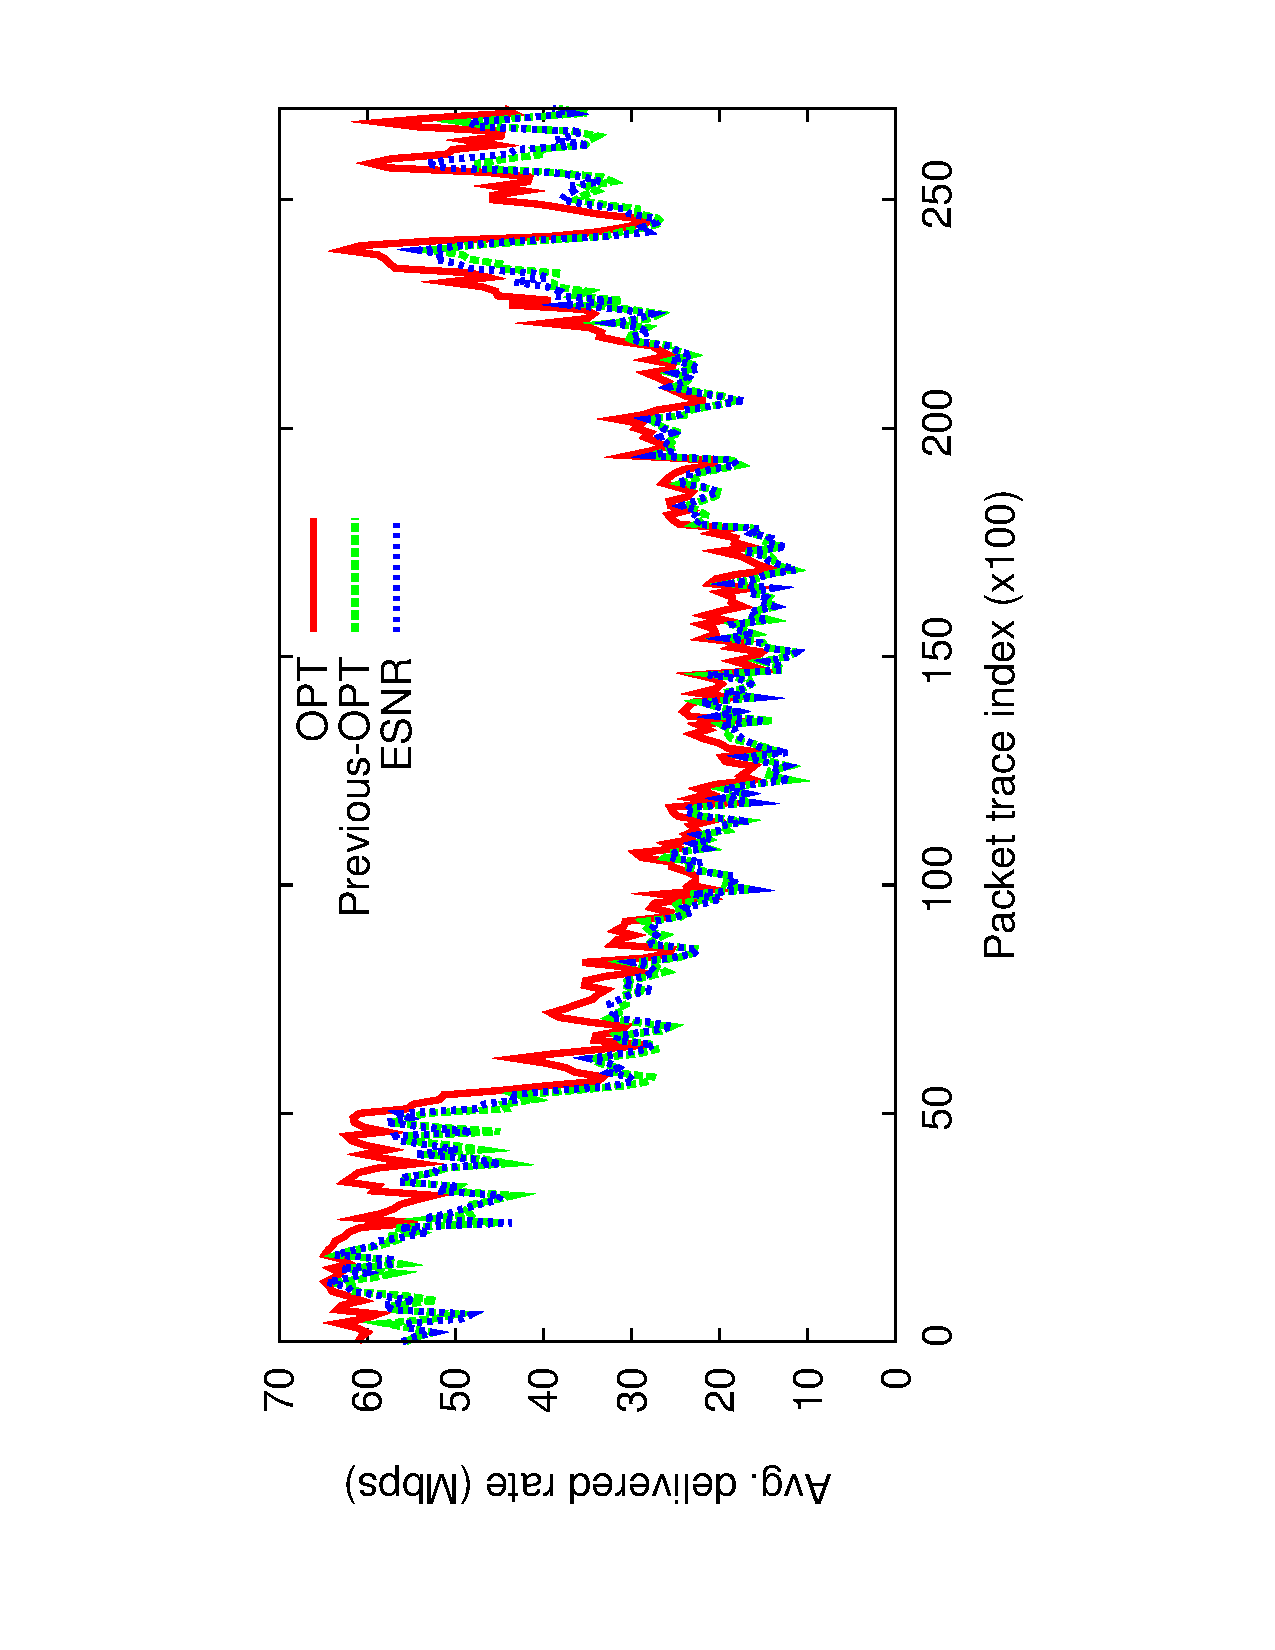
\includegraphics[angle=-90,viewport=120 68 491 760,clip,width=0.95\columnwidth]{figures/esnr/siso_rate_time_opt_eff.pdf}
      \caption{\label{fig:siso_rate_time_opt_eff} OPT and ESNR SISO performance in human-speed mobility.}
\end{figure}

\begin{figure}[t]
      \centering
      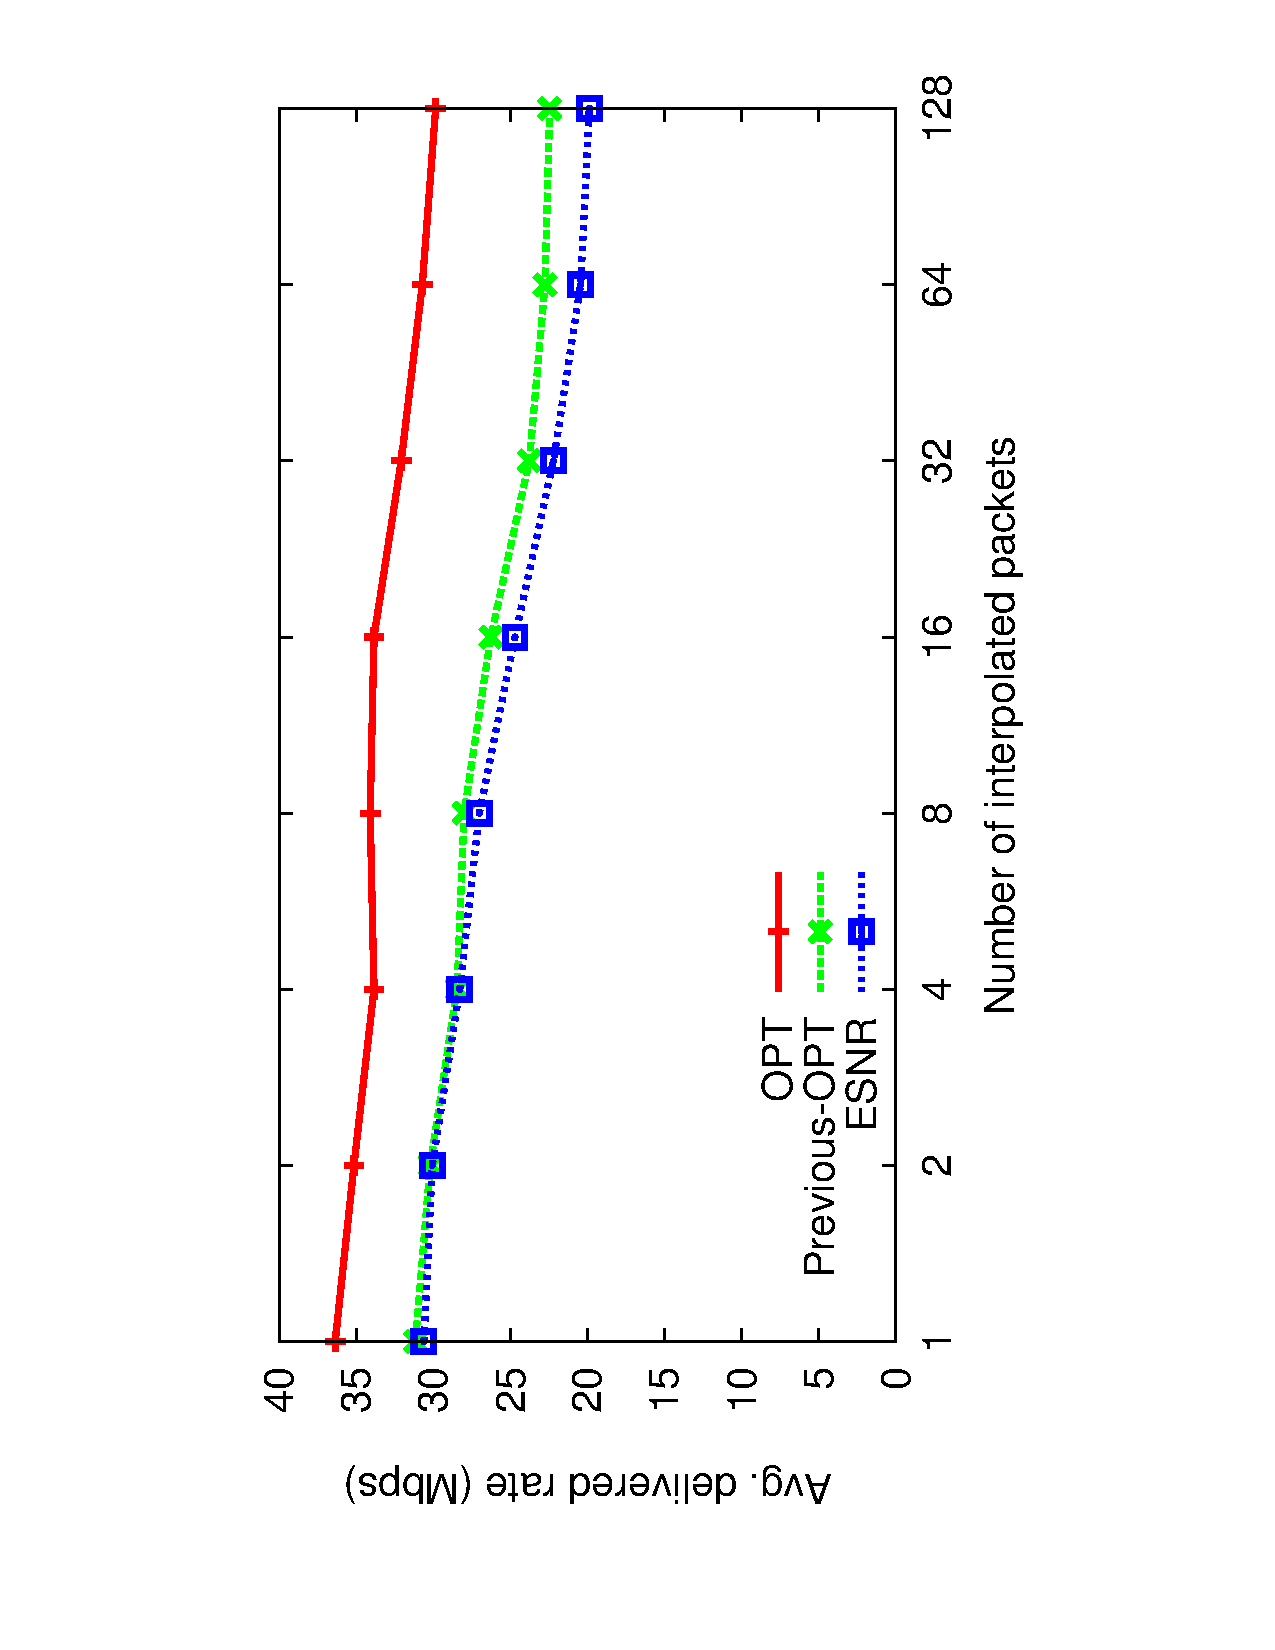
\includegraphics[angle=-90,viewport=120 68 491 760,clip,width=0.95\columnwidth]{figures/esnr/siso_rate_skip_opt_eff.pdf}
      \caption{\label{fig:siso_rate_skip_opt_eff} OPT and ESNR SISO performance in fast mobile channels.}
\end{figure}



\section{Rate Adaptation Results}
\topheading{SISO Performance.} We first examine the performance of ESNR for SISO rates. \figref{fig:siso_rate_time_opt_eff} shows the rate over time for ESNR and OPT over our trace. The performance metric is the average rate over an interval because each algorithm gets an opportunity to send a packet at the same point in the trace. The rate is averaged over a window of 100 packets to smooth the data for readability. ESNR performs excellently. It is below OPT but consistently overlaps Previous-OPT, which is an upper bound for schemes that track the channel and do not predict the future. ESNR is accurate on 75\% of packets, with the expected 10\% target over-selection.

\figref{fig:siso_rate_skip_opt_eff} shows the effects of mobility on SISO channels. Each line plots the average rate as a function of the speed at which we play the trace. We cover a large range of speeds to show trends, in doubling increments from 1$\times$ (walking speed, $\approx$3\mph) to 128$\times$ ($>$300\mph). All schemes fall off with increased speed, and the gap between OPT and Previous-OPT grows from 20\% at human speeds to 1/3 at the fastest speeds. However, even in these mobile channels, ESNR holds up very well and tracks Previous-OPT within 10\%.
Note that packet SNR was observed to fare quite poorly~\cite{Vutukuru_SoftRate} in mobile channels, but since effective SNR reflects actual link quality its estimates are more accurate (\chapref{chap:delivery}) and stable (2--3$\times$ less variance).
%Note this is much better than trained SNR techniques~\cite{Vutukuru_SoftRate}, because packet SNR primarily reflects strong subcarriers, while effective SNR reflects actual performance and is hence more stable.

\heading{SISO Comparison.}
Next, we compare ESNR with SampleRate and SoftRate %. The corresponding rate versus time and rate versus mobility speedup graphs are shown 
in \figref{fig:siso_rate_time_opt_eff_sr_so} and \figref{fig:siso_rate_skip_opt_eff_sr_so}. While it is hard to separate the lines on the graph, at 1$\times$ speed, ESNR slightly outperforms SampleRate which slightly outperforms SoftRate. These results surprised us: SampleRate performs better than we expected, and SoftRate performs less well. 

SampleRate's lagging channel estimate makes it degrade fastest with increasing mobility. However, it maintains a 10--25\% margin with ESNR, still performing well even with large speedups. In deeper analysis, we discovered that dropping rate on retry is an important factor that gives it short-term adaptability. Without this rate fallback (the ``SampleRate fixed'' line), it loses 25--50\% of its performance.

SoftRate has among the slowest falloff with mobility speedup because it directly and accurately measures the channel, and performs the best at maximum speed. However, at slow speeds it is slightly slower on average than SampleRate, though it easily beats a SampleRate without fallback that was the basis for earlier comparisons.\footnote{M. Vutukuru, personal communication, and code inspection.}
We do not believe this gap is fundamental, as SoftRate's post-decoding BER estimate should match or even slightly improve on ESNR\@. Further tuning will likely improve SoftRate. Note that the task for SoftRate is harder in our setting than in the original evaluation. We have added QAM-64 and other coding rates, so it must now chose among 8 SISO rates.

Finally, while the performance differences between schemes are significant, they are always less than a factor of two (ignoring OPT). To put this in perspective, note that other evaluations have reported throughput based on TCP traffic, which will magnify performance gaps by reacting to packet loss.


\begin{figure}[t]
      \centering
      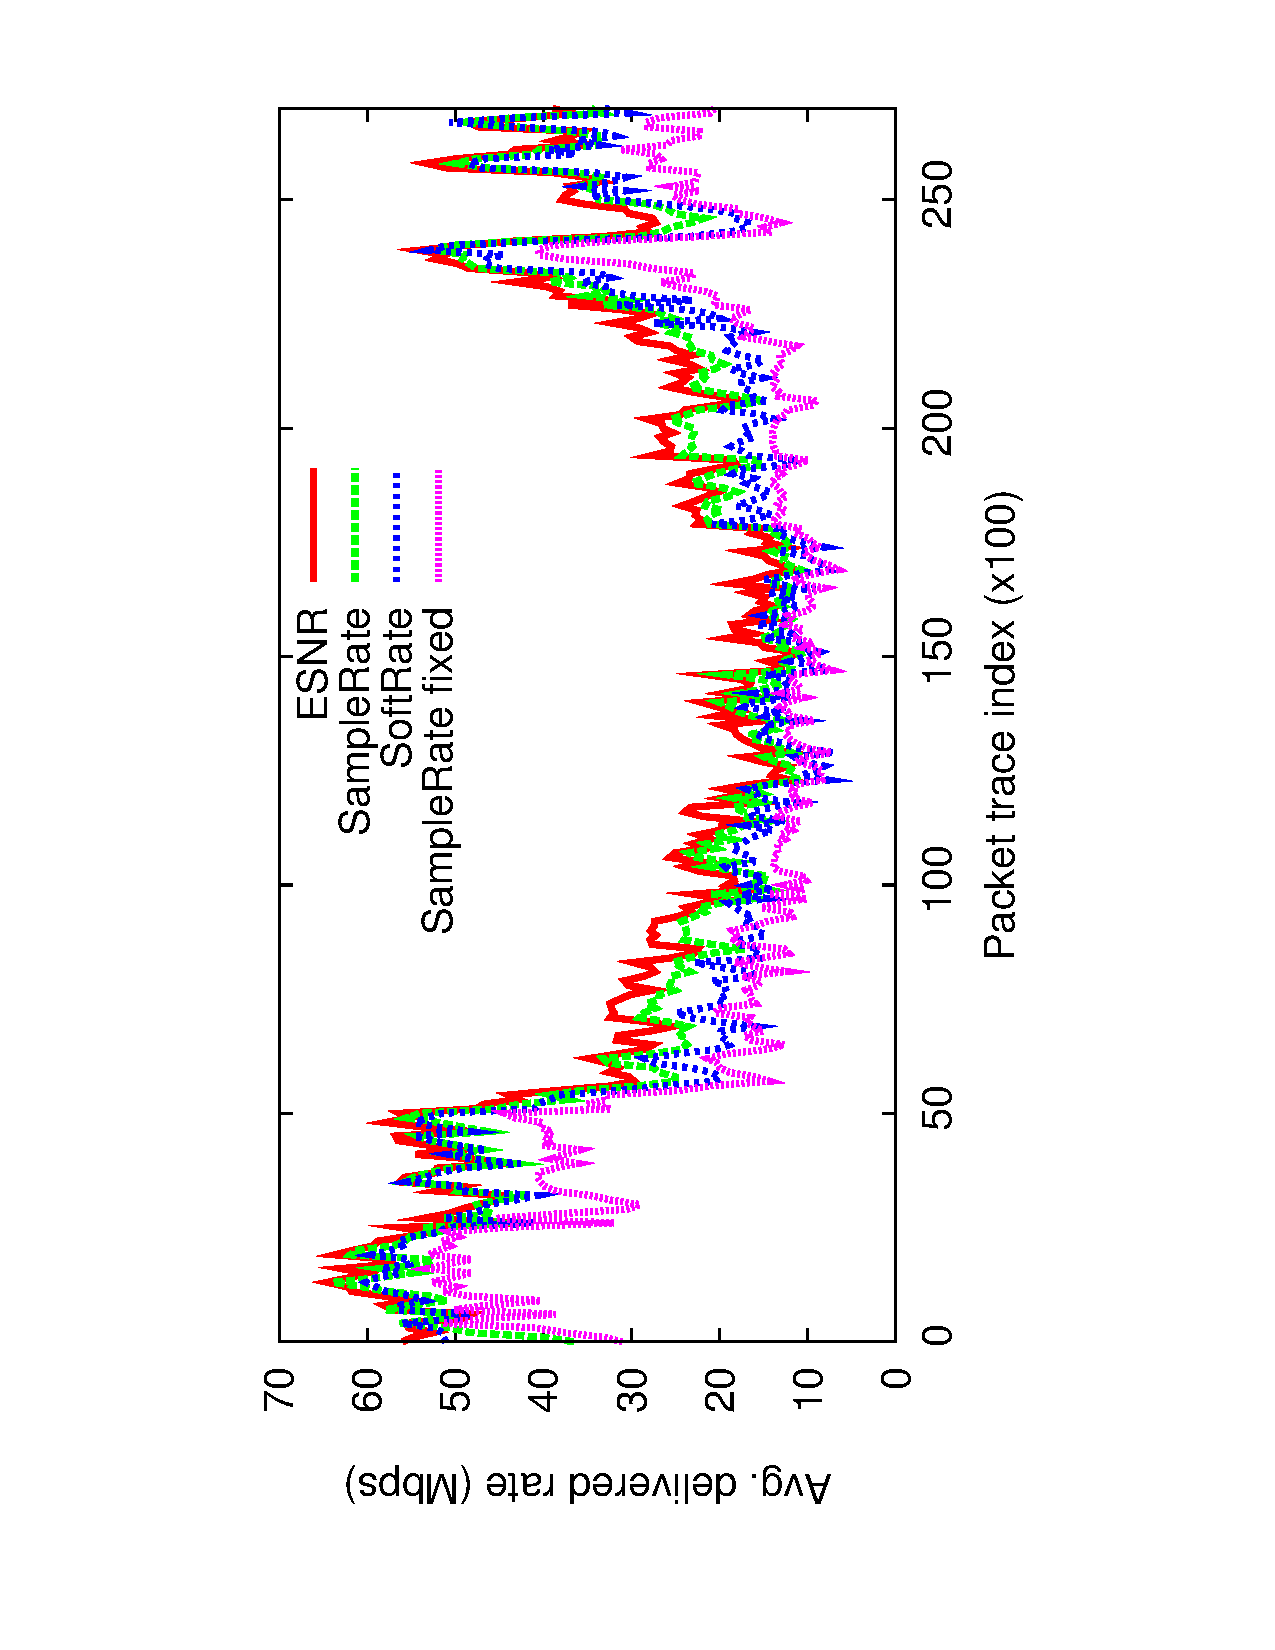
\includegraphics[angle=-90,viewport=120 68 491 760,clip,width=0.95\columnwidth]{figures/esnr/siso_rate_time_opt_eff_sr_so.pdf}
      \vspace{-2pt}
      \caption{\label{fig:siso_rate_time_opt_eff_sr_so} ESNR, SampleRate, and SoftRate SISO performance in human-speed mobility.}
      \vspace{-2pt}
\end{figure}

\begin{figure}[t]
      \centering
      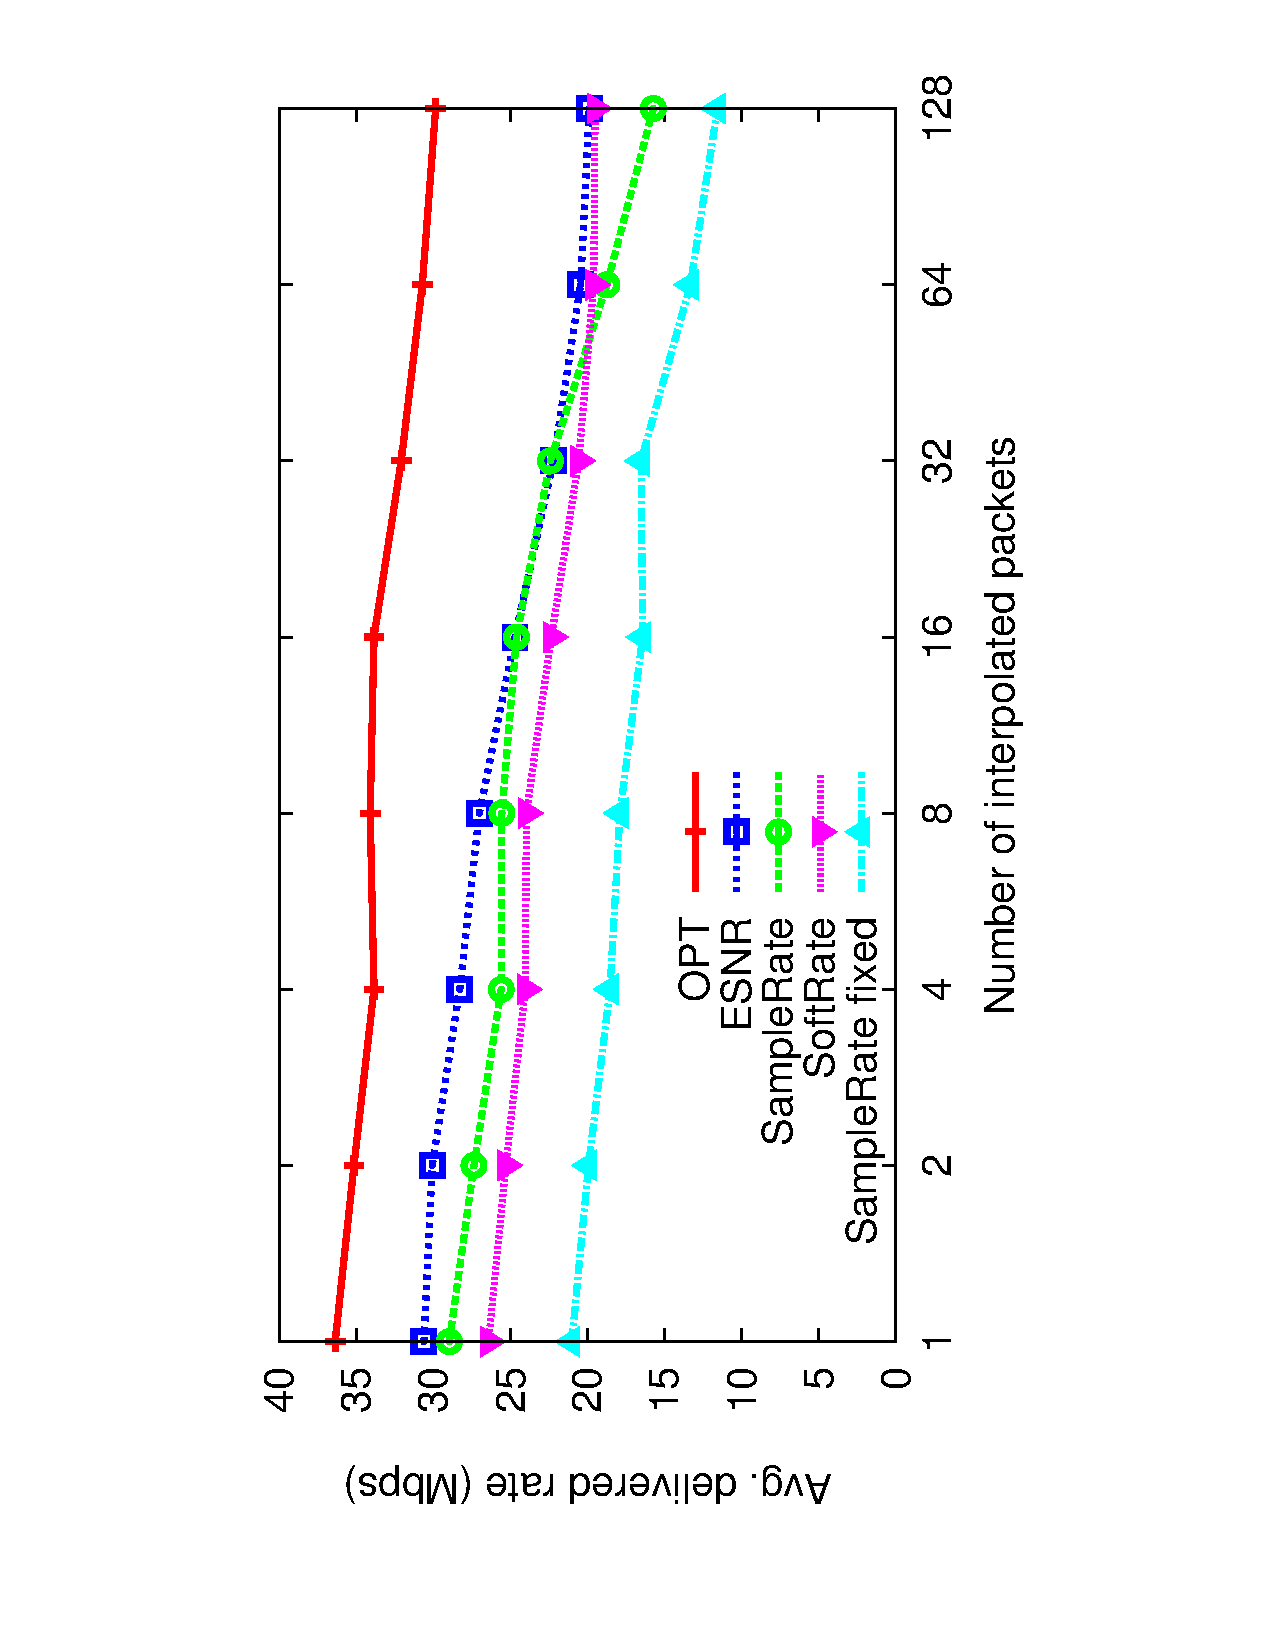
\includegraphics[angle=-90,viewport=120 68 491 760,clip,width=0.95\columnwidth]{figures/esnr/siso_rate_skip_opt_eff_sr_so.pdf}
      \vspace{-2pt}
      \caption{\label{fig:siso_rate_skip_opt_eff_sr_so} OPT, ESNR, SampleRate, and SoftRate SISO performance in fast mobile channels.}
      \vspace{-2pt}
\end{figure}


\begin{figure}[t]
      \centering
      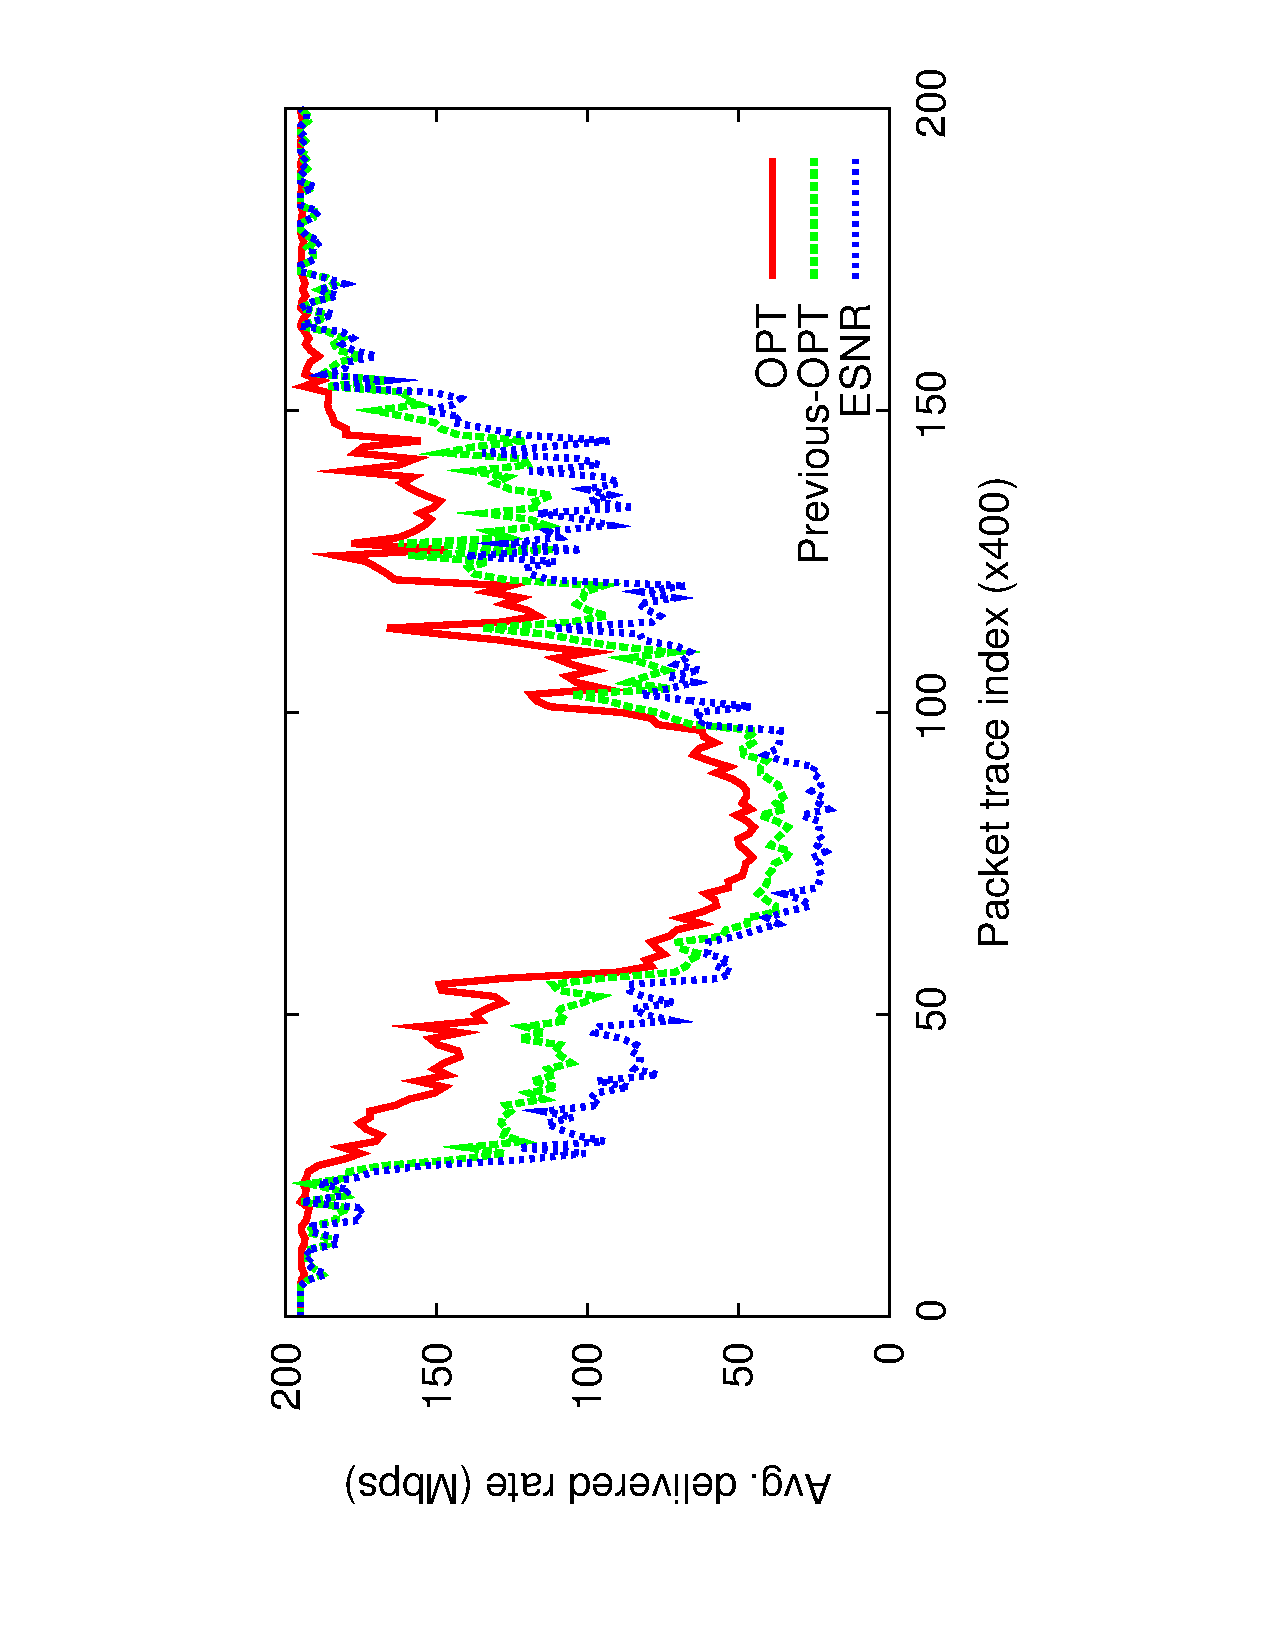
\includegraphics[angle=-90,viewport=125 68 491 760,clip,width=.95\columnwidth]{figures/esnr/mimo_skip_time.pdf}
      \vspace{-2pt}
      \caption{\label{fig:mimo_eff_snr_time} OPT and ESNR MIMO performance in human-speed mobility.}
\end{figure}

\begin{figure}[t]
      \centering
      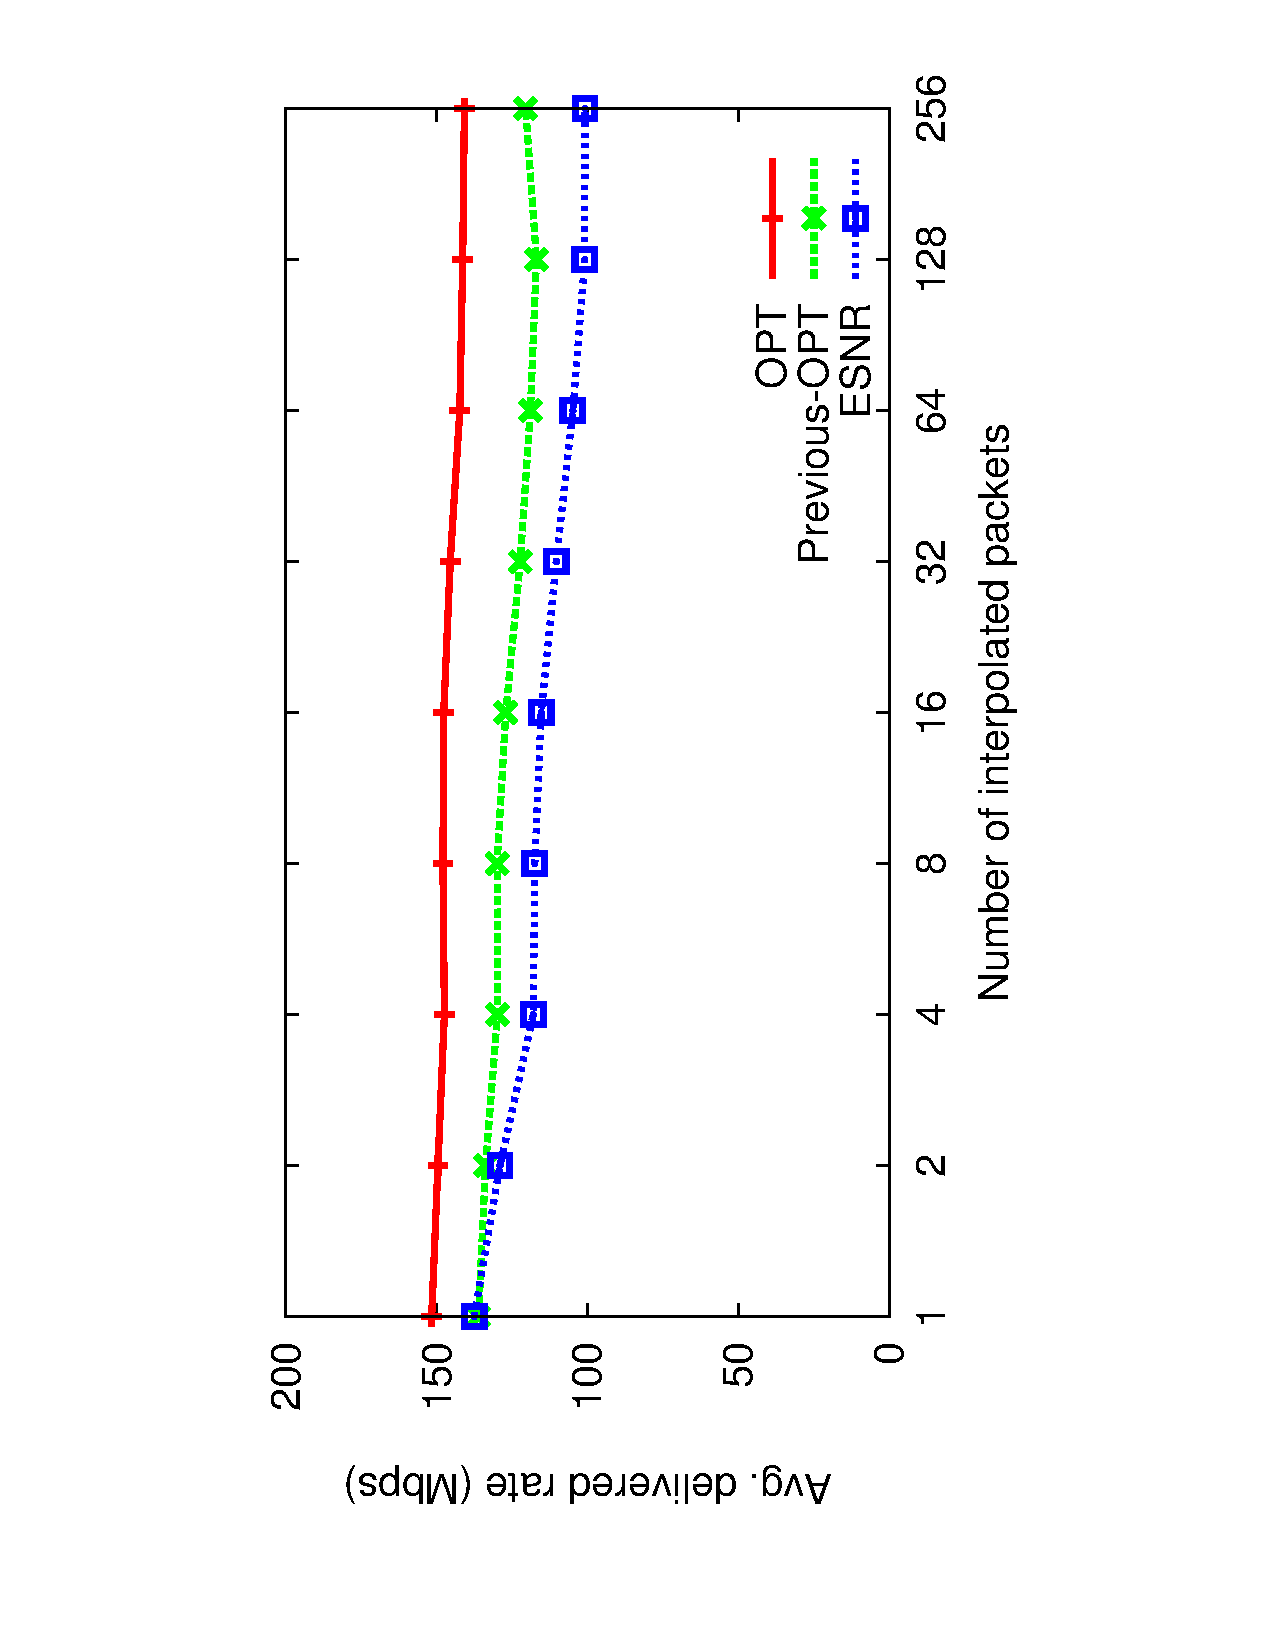
\includegraphics[angle=-90,viewport=125 68 491 760,clip,width=.95\columnwidth]{figures/esnr/mimo_rate_skip.pdf}
      \vspace{-2pt}
      \caption{\label{fig:mimo_eff_snr_speedup} OPT and ESNR MIMO performance in faster mobile channels.}
      \vspace{-2pt}
\end{figure}

\heading{MIMO Performance.}
To show the generality of our model, Figures~\ref{fig:mimo_eff_snr_time} and \ref{fig:mimo_eff_snr_speedup} show the performance of an unmodified ESNR algorithm running for 802.11n MIMO rates. These results do not include SampleRate or SoftRate as they are SISO schemes. Instead, we use OPT as our benchmark.
%\figref{fig:mimo_eff_snr_time} and \figref{fig:mimo_eff_snr_speedup} show the rate versus time and rate versus speedup graphs. 
These figures are in the same form as for SISO, except the range of rates has grown by a factor of 3 to support up to 195\Mbps. 

The trends in these graphs are similar to those in the SISO graphs: at human mobility speeds, ESNR tracks Previous-OPT and delivers excellent performance, with 80\% accuracy and 10\% over-selection. In faster mobile channels, there is a slightly larger gap with Previous-OPT for MIMO than for SISO, likely because ESNR must now choose between 24 rates instead of 8. It is more likely to choose rates under the highest rate that would have worked. 

Finally, note that with 3 antennas there are only four two- and three-stream rates over 117\Mbps (130, 156, 175.5 and 195 Mbps). The visible gap between indices 25--50 in \figref{fig:mimo_eff_snr_time} reflects only the difference between 1 or 2 rates of potentially different antenna modes. Taken together, these results imply that ESNR's MIMO performance is highly competitive.


\heading{Enhancements.}
One strength of our model is that it can accommodate choices other than rates. This lets us add other functionality to ESNR without increasing complexity. We demonstrated an example enhancement to trim excess transmit power in \chapref{chap:delivery}.
% Our example in \secref{sec:delivery} showed that our model has sufficient predictive power to do this. 

A second enhancement is to select the best transmit antenna when there are spare antennas. %A common scenario is an 802.11n AP sending to an 802.11a/g client. The
An 802.11n AP can select antennas to use to send packets to a legacy 802.11a/g client (plus use all antennas to receive packets). With three antennas to choose from, the expected gain in SNR is a little over 2.5\dB~\cite{Goldsmith}. This is often enough to advance to a higher rate.

We ran a version of SISO ESNR that chose the antenna with the highest ESNR for the next transmission. This gave a gain in the average rate of 5\%.  For comparison, OPT achieved a 10\% increase by always knowing which antenna was best. No other rate adaptation schemes directly support these enhancements.

%%%%%%%%%%%%%%%%%%%%%%%%%%%%%%%%%%
\ifx\mainfile\undefined
%
% ==========   Bibliography   ==========
%
%\nocite{*}   % include everything in the uwthesis.bib file
\bibliographystyle{plain}
\bibliography{dhalperi_thesis}

\end{document}
\fi

\ifx\mainfile\undefined
%  ========================================================================
%  Copyright (c) 2006-2011 The University of Washington
%
%  Licensed under the Apache License, Version 2.0 (the "License");
%  you may not use this file except in compliance with the License.
%  You may obtain a copy of the License at
%
%      http://www.apache.org/licenses/LICENSE-2.0
%
%  Unless required by applicable law or agreed to in writing, software
%  distributed under the License is distributed on an "AS IS" BASIS,
%  WITHOUT WARRANTIES OR CONDITIONS OF ANY KIND, either express or implied.
%  See the License for the specific language governing permissions and
%  limitations under the License.
%  ========================================================================
%
 
\documentclass [11pt, twoside] {uwthesis}

\usepackage{color}
\usepackage{url}
\usepackage{amsmath}
\usepackage{amsfonts}
\usepackage[bookmarks,
	hidelinks,
	plainpages=false,
	pdfpagelabels,
	pagebackref=true,
            ]{hyperref}
\renewcommand*{\backref}[1]{}% for backref < 1.33 necessary
\renewcommand*{\backrefalt}[4]{%
  \ifcase #1 %
    (No citations.)%
  \or
    (Cited on page #2.)%
  \else
    (Cited on pages #2.)%
  \fi
}

\newcommand{\biburl}[1]{{\tt<}\url{#1}{\tt>}}

\hypersetup{%
pdfauthor = {Daniel Chaim Halperin},
pdftitle = {Simplifying the Configuration of 802.11 Wireless Networks with Effective SNR},
pdfsubject = {Ph.D. Dissertation},
pdfkeywords = {},
pdfcreator = {University of Washington, Computer Science and Engineering},
pdfproducer = {},
bookmarksopen = {true},
pdfpagelayout = {TwoColumnRight},
}

\usepackage{footnotebackref}
%%%%%%%%%%%%%%%%%%%%%%%%%%%%%%%%%%%%%%%%%%%%%%%%%%%%%%
%%%        Formatting sections                     %%%
%%%%%%%%%%%%%%%%%%%%%%%%%%%%%%%%%%%%%%%%%%%%%%%%%%%%%%
\newcommand{\algref}[1]{Algorithm~\ref{#1}}
\newcommand{\chapref}[1]{Chapter~\ref{#1}}
\renewcommand{\eqref}[1]{Equation~\ref{#1}}
\newcommand{\figref}[1]{Figure~\ref{#1}}
\newcommand{\secref}[1]{\S\ref{#1}}
\newcommand{\tabref}[1]{Table~\ref{#1}}
\newcommand{\heading}[1]{\vspace{4pt}\noindent\textbf{#1}}
\newcommand{\topheading}[1]{\noindent\textbf{#1}}
\newcommand{\noheading}[0]{\vspace{4pt}\noindent}

%%%%%%%%%%%%%%%%%%%%%%%%%%%%%%%%%%%%%%%%%%%%%%%%%%%%%%
%%%        XXX and other warnings                  %%%
%%%%%%%%%%%%%%%%%%%%%%%%%%%%%%%%%%%%%%%%%%%%%%%%%%%%%%
\newcommand{\xxx}[1]{\textit{\color{red}XXX #1}}

%%%%%%%%%%%%%%%%%%%%%%%%%%%%%%%%%%%%%%%%%%%%%%%%%%%%%%
%%%        Units                                   %%%
%%%%%%%%%%%%%%%%%%%%%%%%%%%%%%%%%%%%%%%%%%%%%%%%%%%%%%
\usepackage{xspace}
\newcommand{\unitsep}{\texorpdfstring{\,}{ }}
\def\unit#1{% from: http://www.tex.ac.uk/cgi-bin/texfaq2html?label=csname "Defining a macro from an argument"
  \expandafter\def\csname #1\endcsname{\unitsep\text{#1}\xspace}%
}
\def\varunit#1#2{% from: http://www.tex.ac.uk/cgi-bin/texfaq2html?label=csname "Defining a macro from an argument"
  \expandafter\def\csname #1\endcsname{\unitsep\text{#2}\xspace}%
}
\unit{GHz}
\unit{MHz}
\unit{kHz}
\unit{Gbps}
\unit{Mbps}
\unit{KB}
\unit{dB}
\unit{dBi}
\unit{dBm}
\unit{W}
\unit{mW}
\varunit{uW}{$\mu$W}
\unit{ms}
\varunit{us}{$\mu$s}
\unit{h}
\unit{m}
\unit{s}
\unit{km}
\unit{cm}
\unit{mm}
\varunit{mmsq}{mm$^\text{2}$}
\varunit{insq}{in$^\text{2}$}
\newcommand{\degree}{\ensuremath{^\circ}\xspace}
\newcommand{\degrees}{\degree}
%%%%%%%%%%%%%%%%%%%%%%%%%%%%%%%%%%%%%%%%%%%%%%%%%%%%%%%%%%%%%%%%%%%%%%%%%%%%%%%%%%%%%%
% Euler for math | Palatino for rm | Helvetica for ss | Courier for tt
%
% From: http://www.tug.org/mactex/fonts/LaTeX_Preamble-Font_Choices.html
%%%%%%%%%%%%%%%%%%%%%%%%%%%%%%%%%%%%%%%%%%%%%%%%%%%%%%%%%%%%%%%%%%%%%%%%%%%%%%%%%%%%%%
\renewcommand{\rmdefault}{ppl} % rm
\usepackage[scaled]{helvet} % ss
\usepackage{courier} % tt
\usepackage{eulervm} % a better implementation of the euler package (not in gwTeX)
\normalfont
\usepackage[T1]{fontenc}
%%%%%%%%%%%%%%%%%%%%%%%%%%%%%%%%%%%%%%%%%%%%%%%%%%%%%%%%%%%%%%%%%%%%%%%%%%%%%%%%%%%%%%

%%%%%%%%%%%%%%%%%%%%%%%%%%%%%%%%%%%%%%%%%%%%%%%%%%%%%%
%%%        Figures                                 %%%
%%%%%%%%%%%%%%%%%%%%%%%%%%%%%%%%%%%%%%%%%%%%%%%%%%%%%%
\usepackage{graphicx}
% Caption package both lets you set the spacing between figure and caption
% and also makes the \figref{} point to the right place.
\usepackage[font=bf,aboveskip=6pt,belowskip=-4mm]{caption}
% Allow subfigures, make them bold
\usepackage[bf,BF,small]{subfigure}
% List of figures
\setcounter{lofdepth}{2}  % Print the chapter and sections to the lot

%%%%%%%%%%%%%%%%%%%%%%%%%%%%%%%%%%%%%%%%%%%%%%%%%%%%%%
%%%        Lists with reduced spacing              %%%
%%%%%%%%%%%%%%%%%%%%%%%%%%%%%%%%%%%%%%%%%%%%%%%%%%%%%%
\usepackage{enumitem}

%%%%%%%%%%%%%%%%%%%%%%%%%%%%%%%%%%%%%%%%%%%%%%%%%%%%%%
%%%        Fancy tables                            %%%
%%%%%%%%%%%%%%%%%%%%%%%%%%%%%%%%%%%%%%%%%%%%%%%%%%%%%%
\usepackage{tabulary}
\usepackage{booktabs}

%%%%%%%%%%%%%%%%%%%%%%%%%%%%%%%%%%%%%%%%%%%%%%%%%%%%%%
%%%        Formatting techniques/tools/etc.        %%%
%%%%%%%%%%%%%%%%%%%%%%%%%%%%%%%%%%%%%%%%%%%%%%%%%%%%%%
\newcommand{\term}[1]{\texttt{#1}}

\begin{document}
 
\textpages
\setcounter{chapter}{7} % Set to n-1!
\fi
%%%%%%%%%%%%%%%%%%%%%%%%%%%%%%%%%%

\cleardoublepage
\chapter{Applications of Effective SNR}
\label{chap:esnr_eval}

In the previous chapter, we defined the Effective SNR and showed that it can accurately predict packet delivery for 802.11 rates. In this chapter, we explore applications of Effective SNR to various problems of wireless links and wireless networks.

\begin{table}[htp]
	\centering
	\begin{tabular}{lc}
	\toprule
		\textbf{Application of Effective SNR} & \textbf{Status} \\
	\midrule
		Bitrate/MCS selection & \cite{Halperin_ESNR}\\
		Channel width selection & \cite{Halperin_ESNR}\\
		Antenna selection & \cite{Halperin_ESNR}\\
		Power control & \cite{Halperin_ESNR}\\
		Channel selection & \secref{sec:esnr_chansel}\\
		AP selection & \secref{sec:esnr_apsel}\\
		Path selection/BSS selection in WDS & \secref{sec:esnr_pathsel}\\
		Interference planning \\
		Partial packet recovery/FEC & \cite{Bhartia_FreqDiv}\\
		Beamforming \\
		Multicast rate selection \\
	\bottomrule
	\end{tabular}
	\caption[A variety of applications of Effective SNR]{\label{tab:esnr_uses}A variety of applications of Effective SNR\@.}
\end{table}

\tabref{tab:esnr_uses} shows a list of several potential applications of Effective SNR\@. These range from optimizing various parameters of a single Wi-Fi link, such as the MCS or antenna set used, to coordinating many 802.11 nodes in a dense wireless network. Additionally, we identify applications that can be implemented by looking at other aspects of the Channel State Information in \tabref{tab:csi_uses}. These provide useful primitives that can enable systems to adapt behavior based on the location and movement of the user. Combined, we believe these form the critical building blocks for dense 802.11 networks.

\begin{table}[htp]
	\centering
	\begin{tabular}{lc}
	\toprule
		\textbf{Application of CSI} & \textbf{Status} \\
	\midrule
		Mobility classification & \secref{sec:esnr_mobility}\\
		Indoor localization \\
	\bottomrule
	\end{tabular}
	\caption[A variety of applications of Channel State Information]{\label{tab:csi_uses}A variety of applications of Channel State Information.}
\end{table}

In this chapter, we explore CSI and Effective SNR approaches to implementing four of the above applications.

%%%%%%%%%%%%%%%%%%%%%%%%%%%%%%%%%%%%%%%%%%%%%%%%%%%%%%%%%%%%%%%%%%%%%%%%%%%%%%%%%%%%%%%%%%%%%%%%%%%%%%%%%%%%%%%%%%%%%%%%%%%%%%%%%%%%%%%%%
%%%%%%%%%%%%%%%%%%%%%%%%%%%%%%%%%%%%%%%%%%%%%%%%%%%%%%%%%%%%%%%%%%%%%%%%%%%%%%%%%%%%%%%%%%%%%%%%%%%%%%%%%%%%%%%%%%%%%%%%%%%%%%%%%%%%%%%%%
\section{Channel Selection}\label{sec:esnr_chansel}
Using the new Wi-Fi Direct standard, 802.11 devices that wish to send data directly (instead of through the access point as in 802.11 infrastructure mode) can create a peer-to-peer link. Depending on the amount of interference in the network (e.g., from other clients of the access point) and the quality of the link between the two devices, they may wish to move the link to a different operating channel in order to improve performance. This is one example of the \emph{channel selection} problem: to quickly choose the best operating frequency for a pair of nodes to communicate. In this section, I define the ``best'' channel to be the channel that provides the highest throughput in the absence of interferers.

The channel selection problem is similar to the access point selection problem, and has a similar algorithmic solution (\algref{alg:chan_sel_basic}). It can use the same \fcall{GetMetric} functions for Packet SNR (\algref{alg:snr_link_metric}) and Effective SNR (\algref{alg:eff_snr_link_metric}). The primary difference is a reordering of the parameters: rather than a fixed receiver with fixed channel choosing between multiple senders, a fixed sender and receiver must choose between multiple channels.

%%%%%%%%%%%%%%%%%%%%%%%%%%%%%%%%%%%%%%%%%%%%%%%%
\begin{algorithm}[thp]
\caption{\label{alg:chan_sel_basic}\fcall{ChannelSelection(Channel Set $C$, Sender $s$, Receiver $r$)}}
\begin{algorithmic}[1]
\FORALL{$c \in C$}
\STATE Both $s$ and $r$ switch to channel $c$
\STATE Compute the channel metric $m_c$ using $\fcall{GetMetric}(s,r)$
\ENDFOR
\RETURN $\argmax_{c\in C} m_c$ \hfill \COMMENT{choose the channel with the best metric}
\end{algorithmic}
\end{algorithm}
%%%%%%%%%%%%%%%%%%%%%%%%%%%%%%%%%%%%%%%%%%%%%%%%

%%%%%%%%%%%%%%%%%%%%%%%%%%%%%%%%%%%%%%%%%%%%%%%%%%%%%%%%%%%%%%%%%%%%%%%%%%%%%%%%%%%%%%%%%%%%%%%%%%%%%%%%%%%%%%%%%%%%%%%%%%%%%%%%%%%%%%%%%
\subsection{Characterization of 802.11 Channels}
To start my investigation of channel selection algorithms, I first measured how the operating frequency affects 802.11n links in practice.

As in \secref{sec:esnr_apsel}, I filtered the data to the 11 channels in the 5\GHz band for which there are not co-channel university APs. (Note that channel selection generally makes sense \emph{within} one frequency band. Selection across bands is trivial: due to better antenna gain and Friis' Law effects a 2.4\GHz channel has typically 10\dB--15\dB stronger SNR than a 5\GHz channel for the same nodes.) I further eliminated from consideration any pairs of devices that didn't obtain at least 6.5\Mbps throughput on at least 3 of the 11 channels. This left 201 unidirectional links, approximately a third of the $24*23=552$ unidirectional links in the testbed.

\begin{figure}[t]
	\centering
	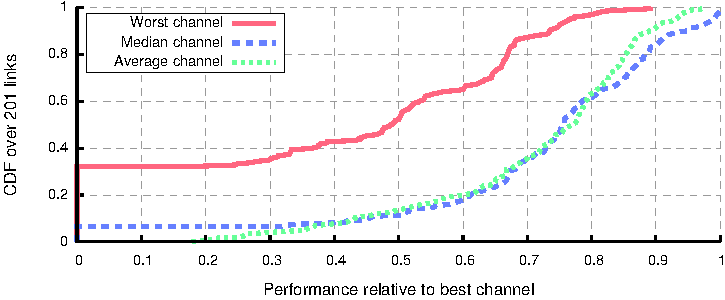
\includegraphics[width=\textwidth]{figures/applications/chan_sel_rel_diff.pdf}
	\caption[The relative difference in throughput over 802.11n channels]{\label{fig:chan_sel_rel_diff}The relative difference in throughput over 802.11n channels.}
\end{figure}

\begin{figure}[t]
	\centering
	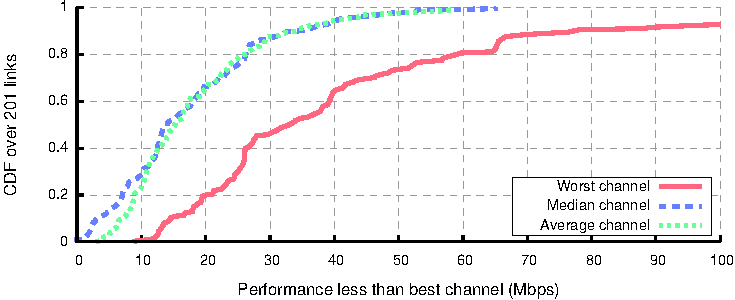
\includegraphics[width=\textwidth]{figures/applications/chan_sel_tpt_diff.pdf}
	\caption[The absolute difference in throughput over 802.11n channels]{\label{fig:chan_sel_tpt_diff}The absolute difference in throughput over 802.11n channels.}
\end{figure}

\subsubsection{Results}
\figref{fig:chan_sel_rel_diff} and \figref{fig:chan_sel_tpt_diff} show how the throughput of the worst, median, and average channels compares to the best channel for these links. Note that because the channel set is fixed and independent of connectivity, the worst channel might deliver no throughput at all---unlike AP selection, in which the client was choosing from only those nodes that responded to its probe. About a third of the links had at least one such channel.

These figures demonstrate that the choice of channel can dramatically impact performance. \figref{fig:chan_sel_rel_diff} shows that the worst channel offers less than half of the best throughput for more than half the links. In absolute terms, this difference can be quite large: the worst channel is a median 33\Mbps worse than the best channel, and for a few links (about 7\%) the difference is more than 100\Mbps. For these links, some channel will deliver no packets at all, while another delivers packets at nearly the maximum bitrate. An unlucky choice of channel can cripple performance and result in little to no throughput.

The median and average channels perform about equivalently in our testbed, and even these are significantly worse. These channels yield less than half the optimal throughput for 15\% of the links and for only one third of links do these come within 80\% of the best throughput. These figures show that for very few links do most channels perform about the same, and the median or average channel is 15\Mbps worse than the best channel for most links, and the gap is larger than 25\Mbps for 20\% of links.

\subsubsection{Signal Strength Across Channels}
Note that the average/median channels are much closer to optimal in these graphs than were the average/median access points we saw in \figref{fig:ap_sel_rel_diff} and \figref{fig:ap_sel_tpt_diff}. Why should this be the case?

I hypothesized that this effect might arise because channels between the same two devices are likely to have similar total signal strengths (i.e., Packet SNR). When two channels have the same signal strength, the difference in performance would come mainly through subchannel fading effects---and while these subchannel effects can affect link quality significantly, as I showed in \chapref{chap:delivery}, the difference is likely not as much as when comparing access points located tens of meters apart.

To test this hypothesis, I analyzed the Packet SNR versus channel for the 11 channels supported by the IWL5300 in the 2.4\GHz band and the 24 channels in the 5\GHz band.\footnote{I used all channels for these experiments, as external interference does not pose a problem. Accurate SNR measurements require only a single packet to be delivered successfully without interference during the preamble.} I considered only links that had at least 10 packets delivered with consistent SNRs and supported at least 3 channels, for a total or 349 links in the 2.4\GHz band and 253 links in the 5\GHz band.

If different channels have similar signal strengths, the Packet SNR will vary only a few dB across the frequency band. \figref{fig:rssi_vs_freq_24} and \figref{fig:rssi_vs_freq_5} plot the normalized Packet SNR for a given link (Packet SNR across all channels minus the average Packet SNR) against channel. The figures include one grey line per link, and the solid black line in each figure shows the median. We see that, indeed, Packet SNR stays within a few dB of the median for most channels. I believe that the shape of the black line in \figref{fig:rssi_vs_freq_5} shows the natural resonance of the antennas, which is consistently non-uniform across the approximately 600\MHz of spectrum the 5\GHz band covers.

\begin{figure}[htp]
	\centering
	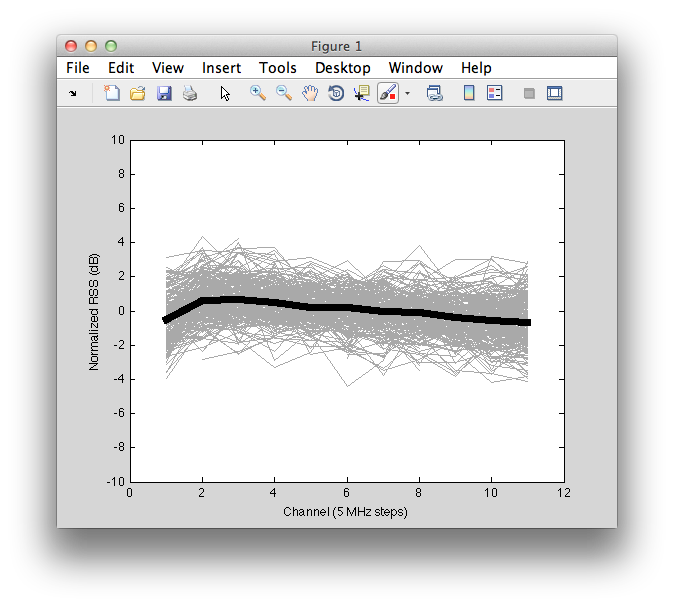
\includegraphics[width=0.6\textwidth]{figures/esnr/rssi_vs_freq_24.png}
	\caption[Normalized Packet SNR versus 2.4\GHz channel for 349 links]{\label{fig:rssi_vs_freq_24}Normalized Packet SNR versus 2.4\GHz channel for 349 links. Solid line shows the median for each channel.}
\end{figure}
\begin{figure}[htp]
	\centering
	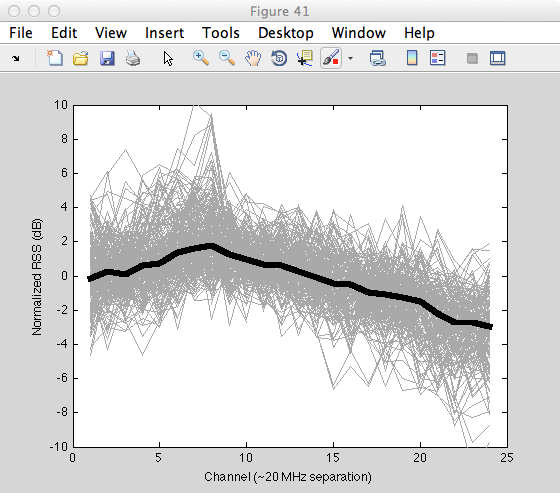
\includegraphics[width=0.6\textwidth]{figures/esnr/rssi_vs_freq_5.png}
	\caption[Normalized Packet SNR versus 5\GHz channel for 253 links]{\label{fig:rssi_vs_freq_5}Normalized Packet SNR versus 5\GHz channel for 253 links. Solid line shows the median for each channel.}
\end{figure}
%\begin{figure}[htp]
%	\centering
%	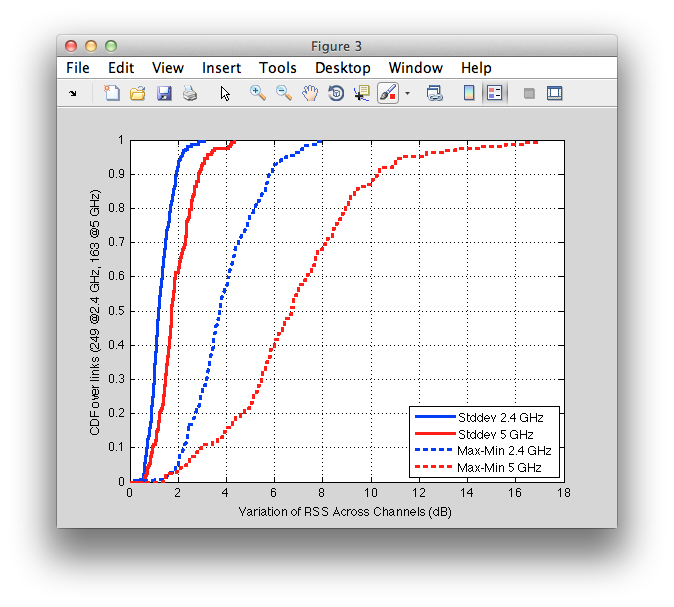
\includegraphics[width=0.6\textwidth]{figures/esnr/rssi_freq_dev.png}
%	\caption{\label{fig:rssi_freq_dev}Standard deviation and max-min spread of Packet SNR across channels within the same band.}
%\end{figure}

From these results, I conclude that a strategy that picks a fixed channel or a random channel will perform significantly worse than a strategy that can identify channels that are likely to offer good performance. Note that this is implicitly the channel selection strategy for strategies that attempt to short-circuit the AP~\cite{Afanasyev_RTSid} used in today's infrastructure networks, because the channel is fixed by the AP. At the same time, because for a fixed link, most channels have roughly the same Packet SNR, fading effects should play a larger role in determining the best channel. This makes the channel selection problem is harder than the AP selection problem, and the solutions may perform slightly worse; however Effective SNR should provide a larger advantage in this case. Having motivated the need for an accurate channel selection algorithm, I present and evaluate different channel selection strategies in the rest of this section.

%%%%%%%%%%%%%%%%%%%%%%%%%%%%%%%%%%%%%%%%%%%%%%%%%%%%%%%%%%%%%%%%%%%%%%%%%%%%%%%%%%%%%%%%%%%%%%%%%%%%%%%%%%%%%%%%%%%%%%%%%%%%%%%%%%%%%%%%%%
%\subsection{Channel Selection Algorithms}
%\algref{alg:chan_sel_basic} is a template for a channel selection algorithm. It takes as input a list of channels to evaluate $C$, and a sender $s$ and receiver $r$ that together define a link. The two nodes hop across channels, using the \fcall{PredictThroughput} function to evaluate the performance of the link on each. The algorithm tracks the best performing channel, labeled $c_{\max}$ and returns that value. (\fcall{ChannelSelection} can also return $\emptyset$ if all channels have zero predicted throughput, but we only consider links that can communicate on at least 1 channel.) Using this template, different channel selection algorithms can be instantiated by providing different implementations of \fcall{PredictThroughput}.
%
%%%%%%%%%%%%%%%%%%%%%%%%%%%%%%%%%%%%%%%%%%%%%%%%%
%\begin{algorithm}[htp]
%\caption{\label{alg:chan_sel_basic}\fcall{ChannelSelection($C, s, r$)}}
%\begin{algorithmic}
%\STATE $t_{\max}\gets 0\Mbps$
%\STATE $c_{\text{best}} \gets \emptyset$
%\FORALL{$c \in C$}
%\STATE Both $s$ and $r$ switch to channel $c$
%\STATE $t \gets \fcall{PredictThroughput($s, r$)}$
%\IF{$t > t_{\max}$}
%	\STATE $t_{\max} \gets t$
%	\STATE $c_{\text{best}} \gets c$
%\ENDIF
%\STATE \textbf{return} $c_{\text{best}}$
%\ENDFOR
%\end{algorithmic}
%\end{algorithm}
%%%%%%%%%%%%%%%%%%%%%%%%%%%%%%%%%%%%%%%%%%%%%%%%%
%
%I consider three different channel selection algorithms in this section. The first is \fcall{ChannelSelectionOPT}, an oracular channel selection algorithm that chooses the optimal channel. For implementation purposes, I instantiate \fcall{ChannelSelectionOPT} by \algref{alg:chan_sel_probe} (\fcall{ProbeChannelThroughput}), which probes all MCSes with MTU-sized packets to determine packet delivery and predicts throughput according to \eqref{eq:prr_throughput}.
%
%%%%%%%%%%%%%%%%%%%%%%%%%%%%%%%%%%%%%%%%%%%%%%%%%
%\begin{algorithm}[tp]
%\caption{\label{alg:chan_sel_probe}\fcall{ProbeThroughput($s, r$)}}
%\begin{algorithmic}
%\STATE $p_0,p_1,\dots,p_{23} \gets 0$
%\STATE $N \gets \text{number of probes at each MCS}$
%\FOR{$i = 1 \dots N$}
%\FOR{$m = 0 \dots 23$}
%\STATE $s$ sends one MTU-sized packet at \mcs{$m$}
%\IF{$s$ receives an ACK from $r$}
%\STATE $p_m \gets p_m + 1$
%\ENDIF
%\ENDFOR
%\ENDFOR
%\STATE $t_{\max}\gets \max \{p_m/N \cdot M(m)\} \text{ over all } m$ \hfill \COMMENT{\eqref{eq:prr_throughput}}
%\STATE \textbf{return} $t_{\max}$
%\end{algorithmic}
%\end{algorithm}
%%%%%%%%%%%%%%%%%%%%%%%%%%%%%%%%%%%%%%%%%%%%%%%%%
%%%%%%%%%%%%%%%%%%%%%%%%%%%%%%%%%%%%%%%%%%%%%%%%%
%\begin{algorithm}[tp]
%\caption{\label{alg:chan_sel_esnr}\fcall{PredictThroughputESNR($s, r$)}}
%\begin{algorithmic}
%\FOR{$m \in \{16, 8, 0\}$}
%\STATE $s$ sends one packet with 0-byte payload at \mcs{$m$}
%\STATE $r$ computes the Effective SNR values $\rho_\text{eff}$ and returns them along with the ACK
%\IF{$s$ receives an ACK from $r$}
%	\STATE \textbf{return} \fcall{ESNRToThroughput}($\rho_\text{eff}$), $\rho_\text{eff}$ \hfill \COMMENT{$\rho_\text{eff}$ is used to break ties}
%\ENDIF
%\ENDFOR
%\STATE \textbf{return} 0
%\end{algorithmic}
%\end{algorithm}
%%%%%%%%%%%%%%%%%%%%%%%%%%%%%%%%%%%%%%%%%%%%%%%%%
%
%The second algorithm chooses the channel based on RSS, presented in \algref{alg:chan_sel_rss}. In this case, the sender only needs to send a single probe packet (with no payload) in order to measure the RSS on the channel. Since \fcall{RSSToThroughput} is monotonically increasing in RSS, this algorithm is equivalent to selecting the channel with the maximum RSS\@.
%
%The third algorithm chooses the channel based on the Effective SNR, presented in \algref{alg:chan_sel_esnr}. Here, the sender sends probes (with no payload) with decreasing numbers of spatial streams to enable the receiver to collect a maximal CSI measurement. The receiver then sends the computed Effective SNR values back to the sender, which uses them to predict the best rate.
%
%I evaluate these three algorithms in the next section.

%%%%%%%%%%%%%%%%%%%%%%%%%%%%%%%%%%%%%%%%%%%%%%%%%%%%%%%%%%%%%%%%%%%%%%%%%%%%%%%%%%%%%%%%%%%%%%%%%%%%%%%%%%%%%%%%%%%%%%%%%%%%%%%%%%%%%%%%%
\subsection{Channel Selection Accuracy}
I evaluate Packet SNR and Effective SNR-based channel selection algorithms based on \algref{alg:chan_sel_basic} and using the link metric functions described in \algref{alg:snr_link_metric} (Packet SNR) and \algref{alg:eff_snr_link_metric} (Effective SNR).

\figref{fig:chan_sel_ratio_opt} shows the performance relative to the optimal algorithm when using Effective SNR or Packet SNR to choose between channels, using the same format as I used for access point selection in \figref{fig:ap_sel_ratio_opt}. Again, we see that both algorithms perform well, though Effective SNR is a better predictor of application performance. Effective SNR chooses an optimal channel for 121 links (60\%), whereas Packet SNR is optimal for only 71 links (35\%). The Effective SNR-based algorithm is within 90\% of optimal for 168 links (84\%), 80\% for 181 links (90\%), and 70\% for 191 links (95\%). In contrast, maximizing the Packet SNR only gets within 90\% of optimal for 112 links (56\%).

\begin{figure}[p]
	\centering
	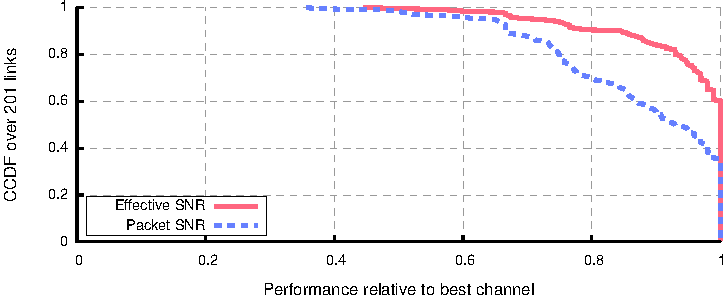
\includegraphics[width=\textwidth]{figures/applications/chan_sel_ratio_opt.pdf}
	\caption[Channel selection algorithm performance relative to Optimal]{\label{fig:chan_sel_ratio_opt}Channel selection algorithm performance relative to an optimal algorithm.}
\end{figure}
\begin{figure}[p]
	\centering
	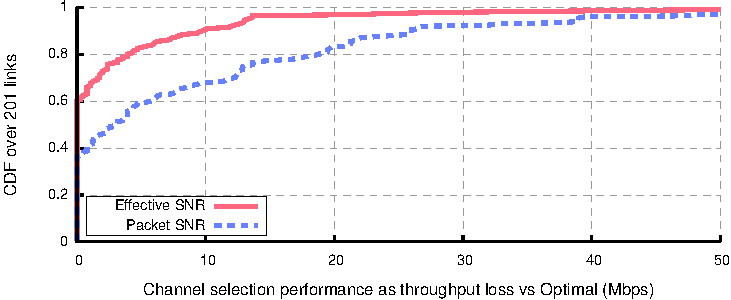
\includegraphics[width=\textwidth]{figures/applications/chan_sel_diff_opt.pdf}
	\caption[Channel selection algorithm performance loss from Optimal]{\label{fig:chan_sel_delta_opt}Channel selection algorithm performance loss from optimal algorithm.}
\end{figure}
\begin{figure}[p]
	\centering
	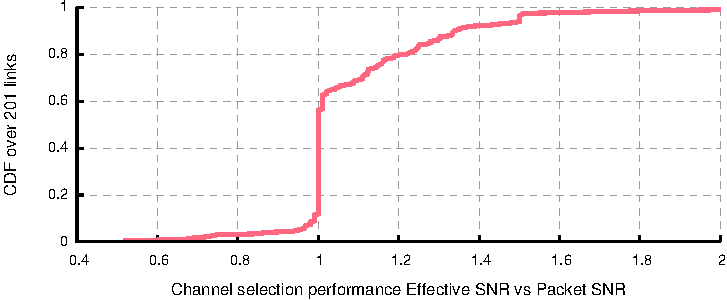
\includegraphics[width=\textwidth]{figures/applications/chan_sel_ratio.pdf}
	\caption[Channel selection algorithm performance with Effective SNR relative to Packet SNR]{\label{fig:chan_sel_ratio}Channel selection performance with Effective SNR relative to Packet SNR.}
\end{figure}

Next, I compare the absolute performance loss of the channel selection algorithms in \figref{fig:chan_sel_delta_opt}. Again, the area over the curves represents the performance lost by each algorithm. This area is 3.3$\times$ larger for the Packet SNR-based selection algorithm, showing that Effective SNR is significantly more accurate. This difference translates to about 9\Mbps faster links when selecting channels via the Effective SNR.

Finally, \figref{fig:chan_sel_ratio} shows the ratio of the performance of the channels selected by Effective SNR and Packet SNR. Recall that a ratio larger than 1 means that Effective SNR chose a faster operating channel. The algorithms choose channels with equal performance for 82 (41\%) of the 201 links, while the Effective SNR-based algorithm chooses a better channel for 94 (47\%) links and the Packet SNR-based algorithm for the remaining 25 (12\%). Additionally, the gains from Effective SNR are much larger than its losses: the Packet SNR strategy chooses a channel that performs 20\% better than the Effective SNR-selected channel for only 4/25 (16\%) links when its channel is better, while Effective SNR chooses a 20\% better channel for 50/94 (53\%) of cases. In other words, the Effective SNR channel selection algorithm is more likely to pick a better channel by a factor of about 4 (94/25), and this difference is more likely to be significant by a factor of about 3 (53\%/16\%).

\heading{Summary.}
These results shows that both Effective SNR- and Packet SNR-based channel selection strategies perform well in my testbed. However, the Effective SNR channel selection strategy is significantly more accurate: it chooses an optimal channel for 70\% more links, it offers about 9\Mbps more per link when selecting suboptimal channels, and it is more likely to choose a better channel than a worse channel by a factor of 4.

Note also that, as hypothesized above, the accuracy of both channel selection algorithms is reduced relative to access point selection. Whereas Effective SNR chose an optimal AP for more than 80\% of clients, it indicates an optimal channel for only 60\% of links; the Packet SNR results exhibit similar a similar decline. This confirms that the similarity of channels leads to more ambiguity when choosing between them. Additionally, the benefits of Effective SNR relative to Packet SNR are larger for channel selection than they were for AP selection. Since most channels have similar Packet SNRs, the real reason for the improvement performance is that my model can accurately assess the impact of subchannel fading effects.

%%%%%%%%%%%%%%%%%%%%%%%%%%%%%%%%%%%%%%%%%%%%%%%%%%%%%%%%%%%%%%%%%%%%%%%%%%%%%%%%%%%%%%%%%%%%%%%%%%%%%%%%%%%%%%%%%%%%%%%%%%%%%%%%%%%%%%%%%%
%\subsection{\xxx{Further Evaluations?}}
%\heading{Channel discrimination.}
%\xxx{how many channels do we need to look at to get good performance?} \figref{fig:rel_diff_draws} shows that, depending on how close to optimal you want to be, need to look at 5, 10, or 15 of the 24 channels in 5\GHz band. If we can evaluate the rate offered by a channel quickly, we can look at more channels in the same amount of time to pick the best rate.
%
%\begin{figure}[htp]
%	\centering
%	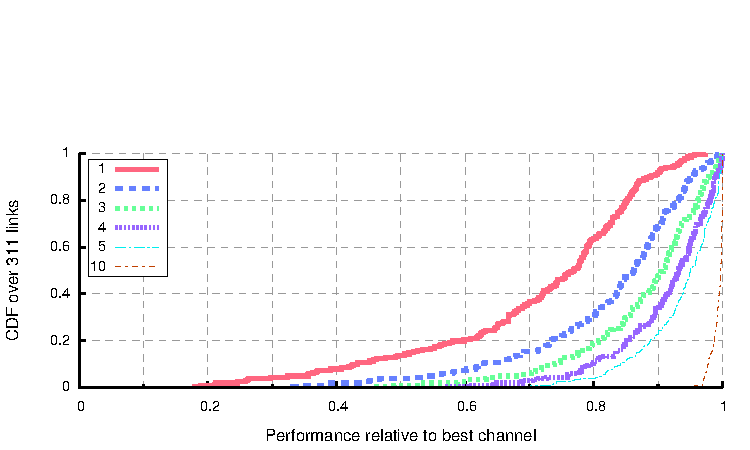
\includegraphics[width=\textwidth]{figures/applications/chan_sel_rel_diff_draws.pdf}
%	\caption[The expected rate after choosing the best of $k$ 802.11n channels]{\label{fig:rel_diff_draws}The expected rate after choosing the best of $k$ 802.11n channels.}
%\end{figure}
%
%\heading{Performance.} \xxx{given time to hop $\mathcal{O}$(1\ms), time to execute a CSI probe $\mathcal{O}$(500\us), and time to execute a rate probe (unknown), how many channels can we look at in $T$ time? Reference \figref{fig:rel_diff_draws} to see what fraction of optimal this enables.}
%
%\heading{Completion Time.} \xxx{The difference between the Effective SNR and the SNR is a proxy for how ``good'' a channel is, based on how flat it is. Given that RSS is similar across channels, the flattest channel will likely offer the best rate. Can we use this to detect a good channel and stop looking early?}
%%%%%%%%%%%%%%%%%%%%%%%%%%%%%%%%%%%%%%%%%%%%%%%%%%%%%%%%%%%%%%%%%%%%%%%%%%%%%%%%%%%%%%%%%%%%%%%%%%%%%%%%%%%%%%%%%%%%%%%%%%%%%%%%%%%%%%%%%
\section{AP selection}\label{sec:esnr_apsel}
In a dense network, a new client may need to select its parent from many available repeaters in addition to the network coordinator. In enterprise AP and Wireless Distribution System networks today, clients typically choose the node whose probe response has the highest SNR\@. (\xxx{though there is heaps of related work doing more complex things.}) In dual-band networks, some devices may prefer a 5\GHz AP with slightly lower SNR, as long as it exceeds a minimum threshold, based on the optimistic assumption that interference is lower in the 5\GHz band. Here, we describe a procedure that uses the Effective SNR to improve this decision process and select a good parent.

Normally, a client scanning for a network cycles through the available channels sends a probe request at the lowest rate (including a single stream and 20\MHz channels), and all APs or repeaters in range respond. We propose that the client instead send multiple probes that use the lowest 6.5\Mbps rate, but vary the number of streams and channel width in decreasing order. In this way, the coordinator and all repeaters that measure CSI from the probes can compute the Effective SNR for the uplink. The probe responses can now include the computed Effective SNR to better inform the client's choice. If the client includes its transmit power level in the probe request (or if the responder makes a conservative estimate), then the responder can combine this information with the CSI measured from the probe to compute the Effective SNR for the downlink. It can then send the probe response at a faster rate than the base rate and reduce the overhead of the probe response.

\subsection{Evaluation methodology}
Compare the following strategies:
\begin{figure}[htp]
	\centering
	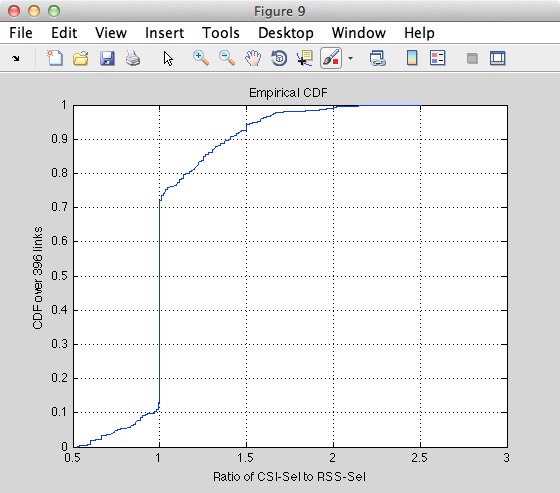
\includegraphics[width=0.6\textwidth]{figures/esnr/ap_sel_ratio.png}
	\caption{\label{fig:ap_sel_ratio}The relative throughput selecting APs by Packet SNR or by Effective SNR\@.}
\end{figure}

\begin{figure}[htp]
	\centering
	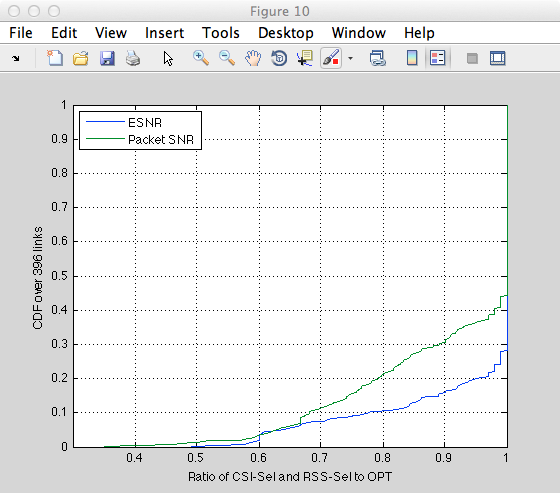
\includegraphics[width=0.6\textwidth]{figures/esnr/ap_sel_ratio_opt.png}
	\caption{\label{fig:ap_sel_ratio_opt}AP selection using Packet SNR or Effective SNR compared to Optimal.}
\end{figure}

\begin{figure}[htp]
	\centering
	\includegraphics[width=0.6\textwidth]{figures/esnr/ap_sel_delta_opt.png}
	\caption{\label{fig:ap_sel_delta_opt}The difference in throughput using APs selected by Packet SNR or Effective SNR compared to Optimal.}
\end{figure}
\begin{itemize}
\item first AP seen
\item max RSSI
\item max CSI predicted rate
\item max measured rate
\end{itemize}

%%%%%%%%%%%%%%%%%%%%%%%%%%%%%%%%%%%%%%%%%%%%%%%%%%%%%%%%%%%%%%%%%%%%%%%%%%%%%%%%%%%%%%%%%%%%%%%%%%%%%%%%%%%%%%%%%%%%%%%%%%%%%%%%%%%%%%%%%
\section{Path selection}\label{sec:esnr_pathsel}
In the last section, we looked at the benefits of AP selection; we now consider the more general problem of path selection. While today's AP and WDS\footnote{Actually, a WDS client implicitly makes a routing decision when joining the network---which access point it chooses can make a large difference in its connection quality.} networks use tree-structured topologies and have only a single path between any two nodes, a future device-to-device wireless network may offer many paths along which packets can be routed. Research in multi-hop routing for wireless mesh networks~\cite{Bahl_repeater,Rodrig_thesis} has shown that the choice of path can effect a large difference in connection quality.

The practical state of the art in this area is the recent work by Bahl et al.~\cite{Bahl_repeater} on an opportunistic repeater scheme for 802.11a. In this design, when a client with a strong link detects rate anomaly~\cite{Heusse_RateAnomaly}---that is, that its throughput is hurt by a client with a weak link monopolizing airtime---the strong client evaluates whether relaying that client's packets would improve throughout for both. In certain scenarios, they showed that this could improve aggregate performance of the network by 50\%--200\%.

While this solution is practical and effective, the use of 802.11n networks significantly complicates the picture. First, the scheme of Bahl et al.\ uses a link's RSSI to select between the 8 available 802.11a rates. In contrast, as we have shown in \chapref{chap:esnr_intro}, RSSI does not accurately predict the rate for 802.11n links, nor does it enable devices to choose between different MIMO modes. Bahl et al.\ used a homogenous network of single-antenna 802.11a chipsets; the set of devices in 802.11n networks includes those with differing numbers of antennas and asymmetric transmit/receive capabilities. While it is not clear how to handle these challenges via the RSSI, the Effective SNR offers the ability to overcome them. In this section, we evaluate the ability of Effective SNR to deliver the benefits of opportunistic repeaters in 802.11n networks.

Note that the problem of path selection does not differ significantly from that of AP selection, except that when choosing between repeaters (or a direct link) the entire path must be considered rather than merely the last hop.\footnote{For simplicity, we assume that the network diameter is small such that pipelining~\cite{Rodrig_thesis} is of limited benefit, and do not consider schemes that forward along multiple unreliable paths such as ExOR~\cite{Biswas_ExOR}.} Instead, in this section we focus on how 802.11n and heterogeneous devices change the opportunities available from relaying, and whether Effective SNR delivers these improvements.

\subsection{Measurements on 802.11a vs 802.11n}
Denote node in center of testbed as AP, and pick a channel. Consider nodes in decreasing order of RSS: have them associate to the network, then turn into repeaters from which the next node can choose. Assume optimal decisions are made at each step. Compare 1x1, 1x3, and 3x3 versions of this scenario.
\begin{itemize}
\item What is the distribution of distance (\#hops) from each node to AP? [How often is repeating used, and at what scale?]
\item What is the distribution of end-to-end tpt? Of the fraction of max (i.e., 65\Mbps or 195\Mbps)? Of the improvement? [This gets at whether the gains get larger or smaller with various device changes.]
\end{itemize}
Same scenario with randomly assigned 3x3, 2x3, and 1x3 devices. How does heterogeneity affect these results?

\subsection{Measurements of Effective SNR}
Perform the same experiments as described above, this time predicting rate by RSSI and then by Effective SNR\@. (Use this only for topology choice, but assume rate selection finds the correct rate.)

%%%%%%%%%%%%%%%%%%%%%%%%%%%%%%%%%%%%%%%%%%%%%%%%%%%%%%%%%%%%%%%%%%%%%%%%%%%%%%%%%%%%%%%%%%%%%%%%%%%%%%%%%%%%%%%%%%%%%%%%%%%%%%%%%%%%%%%%%
\section{Mobility classification}\label{sec:esnr_mobility}
In wireless systems, simply knowing whether a device is mobile can improve performance and reliability. For example, recent work of Ravindranath et al.\ \cite{Ravindranath_SensorHints} demonstrated a system that improved 802.11a performance on a mobile phone by selecting between different bitrate adaptation algorithms based on whether the device was moving. When the device is static, they use algorithms that can conduct a fine-grained search of the rate space to choose the optimum bitrate. When the device is moving, they use an algorithm that performs a coarser search, but does a better job of tracking a moving optimum. In their experiments, the fine-grained algorithms performed 10\%--30\% better in static scenarios, while the coarse-grained algorithm performed 25\%--75\% better in mobile scenarios.

Detecting mobility can also be used to enhance reliability in networks that support dynamic topology, such as today's cellular phone networks, enterprise Wi-Fi wireless distribution systems (WDSes), and networks that support relaying mechanisms such as described above. By proactively looking for a better AP or relay when the device starts moving, service quality can be improved and downtime reduced. \xxx{find some references about cell handoff, WDS handoff, etc.}

The implementation by Ravindranath et al.\ detected mobility using the accelerometer in a mobile phone. While this technique is accurate and responsive, it has a few disadvantages. The use of an on-board sensor means that detection can only be performed by the mobile client, and thus requires protocol changes to communicate a device's mobile state to the other endpoint of the link, and is not backwards-compatible. Also, this technique can only be implemented on devices that have accelerometers, and requires that this sensor be powered on.

In this section, I explore whether it is possible to classify whether a device is mobile based solely on passively measured RF information. If successful, such an implementation would eliminate all of these drawbacks by requiring no extra hardware and supporting unilateral adoption by either endpoint of the link, including the static device. Ravindranath et al.\ made a preliminary attempt to classify mobility using RSSI, but were not successful. They list three challenges: (1) that RSSI is unstable even for static links in a quiet environment; (2) that RSSI varies by different amounts at different absolute signal strengths, and thus needs to be calibrated; and (3) that RSSI was extremely sensitive to movement in the environment and triggered many false hints. Here, I show that the CSI can overcome these challenges and provide a robust solution.

\subsection{Experimental setup}
I configured a SIMO experiment using a single-antenna laptop as the client device, and several of the testbed nodes as three-antenna monitors. The client sent 100,000 back-to-back short packets using MCS~0 (1 stream, 6.5\Mbps), approximately one packet every 300\us for 20\s. In my initial data collection described here, I took four traces. Two of the traces were taken with a \emph{static} client in the UW CSE Networking Lab and students present, but not moving in the room. I then took a trace with \emph{environmental mobility} in which I left the client static, but waved my hand within a few centimeters of the antenna and then walked around the room and opened doors. Finally, I took a \emph{mobile device} trace in which I picked up the laptop and moved it around within a meter of its original location. Chronologically, the traces were taken in the order described within a 10-minute window, with the second static trace taken last. \xxx{These results are from only a single receiver and a single mobile experiment; I could look at more traces and conduct more experiments to flesh out the results and to address claim (2) above.}

\subsection{Evaluation}
\topheading{Classifying mobility with RSS\@.} \figref{fig:mobility_rssi} shows the RSS in dBm measured by one receiver for these four traces. Each line shows the RSS for one of the three receive antennas. I note several interesting effects visible in these measurements. First, the RSS is actually extremely stable in static scenarios. This deviation from Ravindranath et al.\ is likely attributable to the better calibration of the newer 802.11n hardware we use, compared with older hardware used to run experiments with the MadWiFi driver. Second, though RSS does vary with environmental mobility, the variation is fairly small and mostly limited to the periods of activity directly next to the client---later in the trace, when I moved across the room, the RSS variation decreased to the static scenario. It also appears that the variation is not completely correlated across antennas; in several parts of the trace (e.g., at the beginning and around 10--12\s) one or two experience antennas see variation in RSS while the others do not. Finally, the mobile trace exhibits the RSS variation with the largest magnitude, and shows consistent variation throughout the trace and across all antennas. Based on this visual evidence, I conclude it likely that the static scenario can be identified using RSS, and hypothesize that it may also be possible to distinguish between environmental and device mobility. However, I deferred from exploring this possibility further because, as I will show next, the CSI can conclusively classify a device's activity into these three states.

\begin{figure}[htp]
	\centering
	\includegraphics[width=\textwidth]{figures/esnr/mobility_rssi.png}
	\caption{\label{fig:mobility_rssi}RSSI variation in different mobility scenarios.}
\end{figure}

\heading{Classifying mobility with CSI\@.} Here, we examine the same four traces through the lens of the CSI\@. To start, recall that the RSSI yields a single power measurement per sample, whereas the CSI gives a 3-D matrix of complex numbers that represent magnitude and phase on spatial paths and frequency. To quantify the deviation in RSSI, we can simply look at its variation---e.g., absolute difference between samples, or windowed variance---over time. In contrast, we first need a method to quantify the variation in the CSI over time. One simple approach is to use the Pearson correlation function for each spatial path between a transmit-receive antenna pair. The Pearson correlation is the ``standard'' correlation function and is defined as
$$
\text{corr}(\vec{x},\vec{y}) = \frac{\sum_{i=1}^n(x_i-\overline{x})(y_i-\overline{y})}{\sqrt{\sum_{i=1}^n(x_i-\overline{x})^2 \sum_{i=1}^n(y_i-\overline{y})^2}}
$$
for $n$-element vectors $\vec{x},\vec{y}$ indexed by $i$ and with respective means $\overline{x}$ and $\overline{y}$. To apply this to CSI, let $\vec{r}_{pt}$ represent the magnitudes of the CSI coefficients across subcarriers for spatial path $p$ at time sample $t$. Then we can quantify the change between sample $t$ and sample $t+1$ by $\text{corr}(\vec{r}_{pt},\vec{r}_{p(t+1)})$.

The correlations for the four traces and for the three received antennas are shown in \figref{fig:mobility_csi}. We see that the static traces show near-perfect correlation, the environmental mobility trace shows a little deviation, and the mobile trace varies wildly with correlations as low as 0.3. \figref{fig:mobility_csi_cdf} shows the CDF of the correlation (combined across antennas) over time. Static traces never show a correlation below 0.98; the trace with environmental mobility never drops to 0.9, and about 3\% of the correlations in the mobile trace are below 0.9. Though the low-correlation outliers occur infrequently, the fact that they are distributed throughout the traces means a windowed thresholding will accurately be able to distinguish between these three states. Note that the mobility state of a device will change slowly---on the order of seconds or longer---and the outliers are frequent enough at this time scale to prevent false negatives.

%In wireless networks today, laptops tend to be ``portable, but not mobile''~\cite{Woodruff_portable}. That is, though they can move from location to location, laptops are infrequently used while actually in motion.

\begin{figure}[htp]
	\centering
	\includegraphics[width=\textwidth]{figures/esnr/mobility_csi.png}
	\caption{\label{fig:mobility_csi}CSI variation as measured by correlation in different mobility scenarios.}
\end{figure}
\begin{figure}[htp]
	\centering
	\includegraphics[width=\textwidth]{figures/esnr/mobility_csi_cdf.png}
	\caption{\label{fig:mobility_csi_cdf}CDF of CSI variation as measured by correlation in different mobility scenarios.}
\end{figure}

%%%%%%%%%%%%%%%%%%%%%%%%%%%%%%%%%%
\ifx\mainfile\undefined
%
% ==========   Bibliography   ==========
%
%\nocite{*}   % include everything in the uwthesis.bib file
\bibliographystyle{plain}
\bibliography{dhalperi_thesis}

\end{document}
\fi
\ifx\mainfile\undefined
%  ========================================================================
%  Copyright (c) 2006-2011 The University of Washington
%
%  Licensed under the Apache License, Version 2.0 (the "License");
%  you may not use this file except in compliance with the License.
%  You may obtain a copy of the License at
%
%      http://www.apache.org/licenses/LICENSE-2.0
%
%  Unless required by applicable law or agreed to in writing, software
%  distributed under the License is distributed on an "AS IS" BASIS,
%  WITHOUT WARRANTIES OR CONDITIONS OF ANY KIND, either express or implied.
%  See the License for the specific language governing permissions and
%  limitations under the License.
%  ========================================================================
%
 
\documentclass [11pt, twoside] {uwthesis}

\usepackage{color}
\usepackage{url}
\usepackage{amsmath}
\usepackage{amsfonts}
\usepackage[bookmarks,
	hidelinks,
	plainpages=false,
	pdfpagelabels,
	pagebackref=true,
            ]{hyperref}
\renewcommand*{\backref}[1]{}% for backref < 1.33 necessary
\renewcommand*{\backrefalt}[4]{%
  \ifcase #1 %
    (No citations.)%
  \or
    (Cited on page #2.)%
  \else
    (Cited on pages #2.)%
  \fi
}

\newcommand{\biburl}[1]{{\tt<}\url{#1}{\tt>}}

\hypersetup{%
pdfauthor = {Daniel Chaim Halperin},
pdftitle = {Simplifying the Configuration of 802.11 Wireless Networks with Effective SNR},
pdfsubject = {Ph.D. Dissertation},
pdfkeywords = {},
pdfcreator = {University of Washington, Computer Science and Engineering},
pdfproducer = {},
bookmarksopen = {true},
pdfpagelayout = {TwoColumnRight},
}

\usepackage{footnotebackref}
%%%%%%%%%%%%%%%%%%%%%%%%%%%%%%%%%%%%%%%%%%%%%%%%%%%%%%
%%%        Formatting sections                     %%%
%%%%%%%%%%%%%%%%%%%%%%%%%%%%%%%%%%%%%%%%%%%%%%%%%%%%%%
\newcommand{\algref}[1]{Algorithm~\ref{#1}}
\newcommand{\chapref}[1]{Chapter~\ref{#1}}
\renewcommand{\eqref}[1]{Equation~\ref{#1}}
\newcommand{\figref}[1]{Figure~\ref{#1}}
\newcommand{\secref}[1]{\S\ref{#1}}
\newcommand{\tabref}[1]{Table~\ref{#1}}
\newcommand{\heading}[1]{\vspace{4pt}\noindent\textbf{#1}}
\newcommand{\topheading}[1]{\noindent\textbf{#1}}
\newcommand{\noheading}[0]{\vspace{4pt}\noindent}

%%%%%%%%%%%%%%%%%%%%%%%%%%%%%%%%%%%%%%%%%%%%%%%%%%%%%%
%%%        XXX and other warnings                  %%%
%%%%%%%%%%%%%%%%%%%%%%%%%%%%%%%%%%%%%%%%%%%%%%%%%%%%%%
\newcommand{\xxx}[1]{\textit{\color{red}XXX #1}}

%%%%%%%%%%%%%%%%%%%%%%%%%%%%%%%%%%%%%%%%%%%%%%%%%%%%%%
%%%        Units                                   %%%
%%%%%%%%%%%%%%%%%%%%%%%%%%%%%%%%%%%%%%%%%%%%%%%%%%%%%%
\usepackage{xspace}
\newcommand{\unitsep}{\texorpdfstring{\,}{ }}
\def\unit#1{% from: http://www.tex.ac.uk/cgi-bin/texfaq2html?label=csname "Defining a macro from an argument"
  \expandafter\def\csname #1\endcsname{\unitsep\text{#1}\xspace}%
}
\def\varunit#1#2{% from: http://www.tex.ac.uk/cgi-bin/texfaq2html?label=csname "Defining a macro from an argument"
  \expandafter\def\csname #1\endcsname{\unitsep\text{#2}\xspace}%
}
\unit{GHz}
\unit{MHz}
\unit{kHz}
\unit{Gbps}
\unit{Mbps}
\unit{KB}
\unit{dB}
\unit{dBi}
\unit{dBm}
\unit{W}
\unit{mW}
\varunit{uW}{$\mu$W}
\unit{ms}
\varunit{us}{$\mu$s}
\unit{h}
\unit{m}
\unit{s}
\unit{km}
\unit{cm}
\unit{mm}
\varunit{mmsq}{mm$^\text{2}$}
\varunit{insq}{in$^\text{2}$}
\newcommand{\degree}{\ensuremath{^\circ}\xspace}
\newcommand{\degrees}{\degree}
%%%%%%%%%%%%%%%%%%%%%%%%%%%%%%%%%%%%%%%%%%%%%%%%%%%%%%%%%%%%%%%%%%%%%%%%%%%%%%%%%%%%%%
% Euler for math | Palatino for rm | Helvetica for ss | Courier for tt
%
% From: http://www.tug.org/mactex/fonts/LaTeX_Preamble-Font_Choices.html
%%%%%%%%%%%%%%%%%%%%%%%%%%%%%%%%%%%%%%%%%%%%%%%%%%%%%%%%%%%%%%%%%%%%%%%%%%%%%%%%%%%%%%
\renewcommand{\rmdefault}{ppl} % rm
\usepackage[scaled]{helvet} % ss
\usepackage{courier} % tt
\usepackage{eulervm} % a better implementation of the euler package (not in gwTeX)
\normalfont
\usepackage[T1]{fontenc}
%%%%%%%%%%%%%%%%%%%%%%%%%%%%%%%%%%%%%%%%%%%%%%%%%%%%%%%%%%%%%%%%%%%%%%%%%%%%%%%%%%%%%%

%%%%%%%%%%%%%%%%%%%%%%%%%%%%%%%%%%%%%%%%%%%%%%%%%%%%%%
%%%        Figures                                 %%%
%%%%%%%%%%%%%%%%%%%%%%%%%%%%%%%%%%%%%%%%%%%%%%%%%%%%%%
\usepackage{graphicx}
% Caption package both lets you set the spacing between figure and caption
% and also makes the \figref{} point to the right place.
\usepackage[font=bf,aboveskip=6pt,belowskip=-4mm]{caption}
% Allow subfigures, make them bold
\usepackage[bf,BF,small]{subfigure}
% List of figures
\setcounter{lofdepth}{2}  % Print the chapter and sections to the lot

%%%%%%%%%%%%%%%%%%%%%%%%%%%%%%%%%%%%%%%%%%%%%%%%%%%%%%
%%%        Lists with reduced spacing              %%%
%%%%%%%%%%%%%%%%%%%%%%%%%%%%%%%%%%%%%%%%%%%%%%%%%%%%%%
\usepackage{enumitem}

%%%%%%%%%%%%%%%%%%%%%%%%%%%%%%%%%%%%%%%%%%%%%%%%%%%%%%
%%%        Fancy tables                            %%%
%%%%%%%%%%%%%%%%%%%%%%%%%%%%%%%%%%%%%%%%%%%%%%%%%%%%%%
\usepackage{tabulary}
\usepackage{booktabs}

%%%%%%%%%%%%%%%%%%%%%%%%%%%%%%%%%%%%%%%%%%%%%%%%%%%%%%
%%%        Formatting techniques/tools/etc.        %%%
%%%%%%%%%%%%%%%%%%%%%%%%%%%%%%%%%%%%%%%%%%%%%%%%%%%%%%
\newcommand{\term}[1]{\texttt{#1}}

\begin{document}
 
\textpages
\setcounter{chapter}{8} % Set to n-1!
\fi
%%%%%%%%%%%%%%%%%%%%%%%%%%%%%%%%%%

\cleardoublepage
\chapter{Related Work}
\label{chap:related}

Related work section.

%%%%%%%%%%%%%%%%%%%%%%%%%%%%%%%%%%
\ifx\mainfile\undefined
%
% ==========   Bibliography   ==========
%
%\nocite{*}   % include everything in the uwthesis.bib file
\bibliographystyle{plain}
\bibliography{dhalperi_thesis}

\end{document}
\fi

\ifx\mainfile\undefined
%  ========================================================================
%  Copyright (c) 2006-2011 The University of Washington
%
%  Licensed under the Apache License, Version 2.0 (the "License");
%  you may not use this file except in compliance with the License.
%  You may obtain a copy of the License at
%
%      http://www.apache.org/licenses/LICENSE-2.0
%
%  Unless required by applicable law or agreed to in writing, software
%  distributed under the License is distributed on an "AS IS" BASIS,
%  WITHOUT WARRANTIES OR CONDITIONS OF ANY KIND, either express or implied.
%  See the License for the specific language governing permissions and
%  limitations under the License.
%  ========================================================================
%
 
\documentclass [11pt, twoside] {uwthesis}

\usepackage{color}
\usepackage{url}
\usepackage{amsmath}
\usepackage{amsfonts}
\usepackage[bookmarks,
	hidelinks,
	plainpages=false,
	pdfpagelabels,
	pagebackref=true,
            ]{hyperref}
\renewcommand*{\backref}[1]{}% for backref < 1.33 necessary
\renewcommand*{\backrefalt}[4]{%
  \ifcase #1 %
    (No citations.)%
  \or
    (Cited on page #2.)%
  \else
    (Cited on pages #2.)%
  \fi
}

\newcommand{\biburl}[1]{{\tt<}\url{#1}{\tt>}}

\hypersetup{%
pdfauthor = {Daniel Chaim Halperin},
pdftitle = {Simplifying the Configuration of 802.11 Wireless Networks with Effective SNR},
pdfsubject = {Ph.D. Dissertation},
pdfkeywords = {},
pdfcreator = {University of Washington, Computer Science and Engineering},
pdfproducer = {},
bookmarksopen = {true},
pdfpagelayout = {TwoColumnRight},
}

\usepackage{footnotebackref}
%%%%%%%%%%%%%%%%%%%%%%%%%%%%%%%%%%%%%%%%%%%%%%%%%%%%%%
%%%        Formatting sections                     %%%
%%%%%%%%%%%%%%%%%%%%%%%%%%%%%%%%%%%%%%%%%%%%%%%%%%%%%%
\newcommand{\algref}[1]{Algorithm~\ref{#1}}
\newcommand{\chapref}[1]{Chapter~\ref{#1}}
\renewcommand{\eqref}[1]{Equation~\ref{#1}}
\newcommand{\figref}[1]{Figure~\ref{#1}}
\newcommand{\secref}[1]{\S\ref{#1}}
\newcommand{\tabref}[1]{Table~\ref{#1}}
\newcommand{\heading}[1]{\vspace{4pt}\noindent\textbf{#1}}
\newcommand{\topheading}[1]{\noindent\textbf{#1}}
\newcommand{\noheading}[0]{\vspace{4pt}\noindent}

%%%%%%%%%%%%%%%%%%%%%%%%%%%%%%%%%%%%%%%%%%%%%%%%%%%%%%
%%%        XXX and other warnings                  %%%
%%%%%%%%%%%%%%%%%%%%%%%%%%%%%%%%%%%%%%%%%%%%%%%%%%%%%%
\newcommand{\xxx}[1]{\textit{\color{red}XXX #1}}

%%%%%%%%%%%%%%%%%%%%%%%%%%%%%%%%%%%%%%%%%%%%%%%%%%%%%%
%%%        Units                                   %%%
%%%%%%%%%%%%%%%%%%%%%%%%%%%%%%%%%%%%%%%%%%%%%%%%%%%%%%
\usepackage{xspace}
\newcommand{\unitsep}{\texorpdfstring{\,}{ }}
\def\unit#1{% from: http://www.tex.ac.uk/cgi-bin/texfaq2html?label=csname "Defining a macro from an argument"
  \expandafter\def\csname #1\endcsname{\unitsep\text{#1}\xspace}%
}
\def\varunit#1#2{% from: http://www.tex.ac.uk/cgi-bin/texfaq2html?label=csname "Defining a macro from an argument"
  \expandafter\def\csname #1\endcsname{\unitsep\text{#2}\xspace}%
}
\unit{GHz}
\unit{MHz}
\unit{kHz}
\unit{Gbps}
\unit{Mbps}
\unit{KB}
\unit{dB}
\unit{dBi}
\unit{dBm}
\unit{W}
\unit{mW}
\varunit{uW}{$\mu$W}
\unit{ms}
\varunit{us}{$\mu$s}
\unit{h}
\unit{m}
\unit{s}
\unit{km}
\unit{cm}
\unit{mm}
\varunit{mmsq}{mm$^\text{2}$}
\varunit{insq}{in$^\text{2}$}
\newcommand{\degree}{\ensuremath{^\circ}\xspace}
\newcommand{\degrees}{\degree}
%%%%%%%%%%%%%%%%%%%%%%%%%%%%%%%%%%%%%%%%%%%%%%%%%%%%%%%%%%%%%%%%%%%%%%%%%%%%%%%%%%%%%%
% Euler for math | Palatino for rm | Helvetica for ss | Courier for tt
%
% From: http://www.tug.org/mactex/fonts/LaTeX_Preamble-Font_Choices.html
%%%%%%%%%%%%%%%%%%%%%%%%%%%%%%%%%%%%%%%%%%%%%%%%%%%%%%%%%%%%%%%%%%%%%%%%%%%%%%%%%%%%%%
\renewcommand{\rmdefault}{ppl} % rm
\usepackage[scaled]{helvet} % ss
\usepackage{courier} % tt
\usepackage{eulervm} % a better implementation of the euler package (not in gwTeX)
\normalfont
\usepackage[T1]{fontenc}
%%%%%%%%%%%%%%%%%%%%%%%%%%%%%%%%%%%%%%%%%%%%%%%%%%%%%%%%%%%%%%%%%%%%%%%%%%%%%%%%%%%%%%

%%%%%%%%%%%%%%%%%%%%%%%%%%%%%%%%%%%%%%%%%%%%%%%%%%%%%%
%%%        Figures                                 %%%
%%%%%%%%%%%%%%%%%%%%%%%%%%%%%%%%%%%%%%%%%%%%%%%%%%%%%%
\usepackage{graphicx}
% Caption package both lets you set the spacing between figure and caption
% and also makes the \figref{} point to the right place.
\usepackage[font=bf,aboveskip=6pt,belowskip=-4mm]{caption}
% Allow subfigures, make them bold
\usepackage[bf,BF,small]{subfigure}
% List of figures
\setcounter{lofdepth}{2}  % Print the chapter and sections to the lot

%%%%%%%%%%%%%%%%%%%%%%%%%%%%%%%%%%%%%%%%%%%%%%%%%%%%%%
%%%        Lists with reduced spacing              %%%
%%%%%%%%%%%%%%%%%%%%%%%%%%%%%%%%%%%%%%%%%%%%%%%%%%%%%%
\usepackage{enumitem}

%%%%%%%%%%%%%%%%%%%%%%%%%%%%%%%%%%%%%%%%%%%%%%%%%%%%%%
%%%        Fancy tables                            %%%
%%%%%%%%%%%%%%%%%%%%%%%%%%%%%%%%%%%%%%%%%%%%%%%%%%%%%%
\usepackage{tabulary}
\usepackage{booktabs}

%%%%%%%%%%%%%%%%%%%%%%%%%%%%%%%%%%%%%%%%%%%%%%%%%%%%%%
%%%        Formatting techniques/tools/etc.        %%%
%%%%%%%%%%%%%%%%%%%%%%%%%%%%%%%%%%%%%%%%%%%%%%%%%%%%%%
\newcommand{\term}[1]{\texttt{#1}}

\begin{document}
 
\textpages
\setcounter{chapter}{9} % Set to n-1!
\fi
%%%%%%%%%%%%%%%%%%%%%%%%%%%%%%%%%%

\cleardoublepage
\chapter{Conclusions and Future Work}
\label{chap:conclusion}

Modern wireless devices can provide flexible, portable, high-performance connectivity at low cost. This unprecedented functionality is poised to enable a new class of rich applications built by combining functionality from many devices. The key missing component is a network connectivity layer that ``just works'', providing good performance overall and quickly adapting to changing application demands and mobile wireless environments.

There are two components to such a network layer. The first is a protocol to connect the devices logically. For the example context of 802.11n, this is readily available in the form of Wi-Fi Direct~\cite{wifi_direct}, a recently standardized specification for building wireless peer-to-peer networks targeted at these applications. Support for Wi-Fi Direct is actively being developed in major consumer operating systems including Linux, Mac OS X, Windows, and Android.

The focus of my thesis is on the second key component: A way to configure the physical layer parameters and network topology to best meet application needs. The nature of modern wireless technology and heterogeneity of wireless devices combined with the inherent multi-device coordination problems that applications necessitate leads to large configuration state spaces from which the network must find a good operating point. In this thesis, I have demonstrated that my Effective SNR model provides a practical mechanism to cut through these large spaces and efficiently configure the physical layer. I have also shown that it can flexibly handle a wide variety of applications and parameters that no prior approaches considered in tandem.

In this chapter I summarize my thesis and its contributions and present next steps for this work.

\section{Thesis and Contributions}
My thesis is that \emph{it is possible to rapidly and accurately predict how well different configurations of MIMO and OFDM wireless links will perform in practice, using a small set of wireless channel measurements}. I demonstrated this thesis by building an Effective SNR-based model for wireless networks and evaluating it in the context of IEEE 802.11n.

My Effective SNR model unifies wireless network configuration using a simple interface, taking as input a MIMO and OFDM channel measurement and transmitter and receiver device configurations, and producing a single output bit that predicts whether that combination will deliver packets. This flexible API can express a wide class of applications, as illustrated by the algorithms I presented in \chapref{chap:delivery}, \chapref{chap:rate}, and \chapref{chap:applications}.

I demonstrated that this model is practical because it has low overhead and can be deployed using commodity wireless hardware today. My model uses measurements already taken by devices in order to receive packets, and can compute its output in much less time than it takes to transmit a packet. In most cases, only a few bytes that represent application decisions need to be exchanged, such as a receiver feeding back a particular requested rate to a transmitter. And my detailed prototype evaluation of the model in a wide variety of applications provides experimental proof that this model is practical and accurate for real devices operating in real wireless channels. I used this prototype to apply model to a wide range of applications, and showed that it has good performance that extends to large search spaces and fast mobile channels.

My specific contributions are as follows.

\begin{itemize}[leftmargin=0.5cm,parsep=1ex,itemsep=1ex,topsep=1ex]
\item First, I developed a model to predict the error performance of different transmitter and receiver configurations on real MIMO-OFDM wireless channels. This model is flexible to support a wide variety of transmitter and receiver device capabilities and applications, and includes considerations of practical factors such as measurement errors, different device implementations, and practical protocols. I also detailed how to use this model in a system that can solve a large number and variety of configuration problems.
\item Second, I presented an implementation of this system in the context of 802.11n using a commodity commercial wireless device. This prototype demonstrated my model's feasibility in practice and handles the practical considerations of operation over real links using real, non-ideal hardware. This includes a detailed experimental evaluation of my system that shows that this model accurately predicts packet delivery over real 802.11n wireless links in practice.
\item Third, I evaluated this system in the context of a wide variety of 802.11n applications, and quantified the application performance gains when using my Effective SNR metric over versions that use the Packet SNR based on RSSI measurements available today.
\item Finally, as part of my thesis I have produced an 802.11n research platform based on open-source Linux kernel drivers, open-source application code, and commodity Intel 802.11n devices using closed-source firmware that I customized.
%that uses commodity 802.11n wireless devices to measure the 802.11n CSI for the wireless channel, and use this tool to apply my model to real measured 802.11n channels.
I have released this tool publicly, and at the time of writing it is in use at 23 universities, research labs, and corporations.
\end{itemize}

\section{Future Work}
In this section, I consider paths for future research.

\subsection{Practical Benefits of Beamforming}
Transmit beamforming is a well-studied area of research in communications theory. Most theoretical systems aim to optimize Shannon capacity using ideal hardware, in which case the well known water-filling approach~\cite[p. 183]{Tse} optimizes performance by allocating power across subchannels proportional to SNR, using the singular value decomposition. This approach may be inefficient in practice for two reasons. First, real transmit hardware can only support signals with a particular dynamic range, and so cannot perfectly support water-filling. Secondly, in practical systems like 802.11, different subchannels are modulated identically and thus cannot make good use of the asymmetric power across subchannels. Instead, the Effective SNR model can be used to evaluate allocations of power with the goal of minimizing bit errors and finding the best working modulation and coding scheme across all subchannels.

\subsection{Spatial Reuse}
Another area of further research is understanding and managing spatial reuse, that is, understanding when multiple transmitters can send concurrently on the same frequency band. This problem is the subject of great importance in today's AP wireless networks, but will likely be ameliorated to a large extent in future wireless networks that can take advantage of multiple channels. Still, existing work has shown large gains from spatial reuse especially in the area of eliminating corner cases of hidden terminals that can degrade link performance to almost nothing. Today's solutions such as CSMA/CA use expensive distributed coordination mechanisms (i.e., RTS/CTS~\cite{Karn_MACA}) with large overheads that are often disabled in practice, and today's research proposals on spatial reuse for Wi-Fi~\cite{Shrivastava_CENTAUR,Vutukuru_CMAP} have simply fixed the entire network to a single rate during experiments because of the large search space. Communications theory has also defined an Effective SINR notion that takes interference into account; extending my model to support a practical version of this notion would likely be useful as well.

\subsection{Saving Energy with Effective SNR}
Effective SNR could be highly integrated into the development of better methods to manage the power consumption of battery-operated devices. In particular, clients could select access points or relays with the express aim of minimizing wake time. By choosing a close relay that uses fast rates, a client can spend less time awake. By disabling receive antennas on the mobile device and using advanced mechanisms such as beamforming on the transmitter, the client can make further power savings. I highlighted the importance of these 802.11n parameters in an earlier measurement study~\cite{Halperin_Power}, but have not performed follow-up research.

\subsection{Integration into Wi-Fi Direct}
Finally, I would like to integrate my thesis into a modern flexible networking system to really build a flexible application layer that ``just works''. The immediately available practical environment is that of Wi-Fi Direct, which is close to being refined enough to support experiments. Though my thesis has demonstrated the practical benefits of my model and its deployment in a variety of individual applications, building a working combined system would provide invaluable practical experience and research lessons.

\section{Summary}
The way that chaotic wireless systems such as 802.11 are configured today relies on probing, for rate adaptation and for a host of other applications. This probing is the standard strategy because communications-theoretic approaches to configuring network parameters are considered too inaccurate to work well. However, in my thesis I have shown the opposite, namely that it is indeed possible to connect theory back to real wireless systems operating in real wireless channels. I have presented an Effective SNR model for wireless systems that use modern physical layer techniques like MIMO and OFDM, and shown that it works well for real wireless devices operating in real wireless channels for the state-of-the-art wireless system in use today, IEEE 802.11n. Going forward, I hope that Effective SNR will be integrated into the control plane for the dense future wireless networks and help enable the next generation of device-to-device wireless applications.

%%%%%%%%%%%%%%%%%%%%%%%%%%%%%%%%%%
\ifx\mainfile\undefined
%
% ==========   Bibliography   ==========
%
%\nocite{*}   % include everything in the uwthesis.bib file
\bibliographystyle{plain}
\bibliography{dhalperi_thesis}

\end{document}
\fi


 

% ==========   End notes   ==========

\printendnotes

%
% ==========   Bibliography   ==========
%
%\nocite{*}   % include everything in the uwthesis.bib file
\bibliographystyle{plain}
\bibliography{dhalperi_thesis}
%
% ==========   Appendices
%
\appendix
\raggedbottom\sloppy
%
% ==========   Vita   ==========
%
\vita{Jim Fox is a Senior Software Engineer at the University of Washington.
His duties do not include maintaining this package.  It is rather
an avocation which he maintains as he deems fit.

He welcomes your comments to {\tt fox@washington.edu}.
}

\end{document}
